% =====================================================================
%  Rapport de stage technicien : AirLiquide GMAO+ (Air Liquide Tunisie, juillet 2026)
%  Fichier principal à compiler : main.tex (compilateur pdfLaTeX, deux passes).
% =====================================================================
\documentclass[11pt,a4paper,oneside]{report}

% =====================================================================
%  Préambule : polices, couleurs, titres, en-têtes, tableaux, figures
% =====================================================================

% --- Langue, encodage, polices (Pagella pour le texte, Heros pour les titres, Cursor pour le code) ---
\usepackage[utf8]{inputenc}
\usepackage[T1]{fontenc}
\usepackage{textcomp}
\usepackage[french]{babel}
\frenchsetup{StandardLists=true}
\usepackage{tgpagella}
\usepackage[scale=0.92]{tgheros}
\usepackage[scale=0.88]{tgcursor}
\usepackage{microtype}

% --- Page ---
\usepackage[a4paper,top=2.8cm,bottom=2.6cm,left=3cm,right=2.5cm,headheight=22pt]{geometry}
\usepackage{setspace}
\setstretch{1.18}
\setlength{\parskip}{0.35em}
\setlength{\parindent}{0pt}

% --- Couleurs (charte du logo Air Liquide) ---
\usepackage[table]{xcolor}
\definecolor{ALbleu}{RGB}{35,72,152}
\definecolor{ALrouge}{RGB}{214,28,52}
\definecolor{ALgris}{RGB}{239,242,247}
\definecolor{ALtexte}{RGB}{105,113,128}

% --- Figures, tableaux, listes ---
\usepackage{graphicx}
\graphicspath{{images/}}
\usepackage{float}
\usepackage{wrapfig}
\usepackage{needspace}
\usepackage{booktabs}
\usepackage{longtable}
\setlength{\LTpre}{0.6em}
\setlength{\LTpost}{0.6em}
\usepackage{caption}
\captionsetup{font={small,sf},labelfont={bf,color=ALbleu},labelsep=endash,skip=6pt}
\captionsetup[table]{position=top,skip=5pt}
\captionsetup[figure]{position=bottom}
\setlength{\intextsep}{10pt plus 2pt minus 2pt}
\usepackage{enumitem}
\setlist{itemsep=0.2em,topsep=0.3em,parsep=0pt,leftmargin=1.4em}
\setlist[itemize,1]{label=\textendash}
\setlist[itemize,2]{label=\textendash}
\usepackage{xurl}

% --- Titres ---
\usepackage{titlesec}
\titleformat{\chapter}[hang]
  {\sffamily\bfseries\color{ALbleu}\fontsize{25}{29}\selectfont}
  {\color{ALrouge}\thechapter}{0.7em}{}[\vspace{5pt}{\color{ALrouge}\titlerule[1.4pt]}]
\titleformat{name=\chapter,numberless}[hang]
  {\sffamily\bfseries\color{ALbleu}\fontsize{25}{29}\selectfont}
  {}{0pt}{}[\vspace{5pt}{\color{ALrouge}\titlerule[1.4pt]}]
\titlespacing*{\chapter}{0pt}{-12pt}{28pt}
\titleformat{\section}{\sffamily\bfseries\Large\color{ALbleu}}{\color{ALrouge}\thesection}{0.6em}{}
\titleformat{\subsection}{\sffamily\bfseries\large}{\thesubsection}{0.6em}{}
\titlespacing*{\section}{0pt}{18pt}{8pt}
\titlespacing*{\subsection}{0pt}{12pt}{5pt}

% --- En-têtes et pieds de page ---
\usepackage{fancyhdr}
\pagestyle{fancy}
\fancyhf{}
\fancyhead[L]{\sffamily\small\color{ALtexte}AirLiquide GMAO+}
\fancyhead[R]{\sffamily\small\color{ALtexte}\nouppercase{\leftmark}}
% Numéro de page centré ; il n'apparaît qu'à partir de l'introduction (\corpstrue dans main.tex)
\newif\ifcorps\corpsfalse
\newcommand{\numpage}{\ifcorps{\sffamily\small\color{ALtexte}\thepage}\fi}
\fancyfoot[C]{\numpage}
\renewcommand{\headrulewidth}{0.5pt}
\renewcommand{\headrule}{\hbox to\headwidth{\color{ALrouge}\leaders\hrule height \headrulewidth\hfill}}
\fancypagestyle{plain}{\fancyhf{}\fancyfoot[C]{\numpage}\renewcommand{\headrulewidth}{0pt}}

% --- Intitulés en français ---
\addto\captionsfrench{\renewcommand{\bibname}{Bibliographie et webographie}}
\addto\captionsfrench{\renewcommand{\listfigurename}{Liste des figures}}
\addto\captionsfrench{\renewcommand{\listtablename}{Liste des tableaux}}
\setlength{\emergencystretch}{2em}

% --- Liens ---
\usepackage[colorlinks=true,linkcolor=ALbleu,urlcolor=ALbleu,citecolor=ALrouge]{hyperref}
\hypersetup{pdftitle={AirLiquide GMAO+ : rapport de stage technicien},pdfauthor={Zakaria Ali Fekih Ahmed}}
\setcounter{tocdepth}{1}


% ---------------------------------------------------------------------
%  Informations de la page de garde
% ---------------------------------------------------------------------
\newcommand{\Auteur}{Zakaria Ali FEKIH AHMED}
\newcommand{\Formation}{Cycle ingénieur en Génie Biomédical, parcours TTIS}
\newcommand{\Organisme}{Air Liquide Tunisie, service Maintenance}
\newcommand{\EncadrantPro}{M. Marouane HASSAN, responsable génie biomédical}
\newcommand{\PeriodeStage}{du 1\textsuperscript{er} juillet au 1\textsuperscript{er} août 2026}
\newcommand{\AnneeUniv}{2025/2026}
\newcommand{\SousTitre}{Conception et réalisation d'une application web de gestion de la maintenance et du service après-vente des dispositifs médicaux respiratoires}

\begin{document}

% ---------- Pages préliminaires (non numérotées : la numérotation commence à l'introduction) ----------
\pagenumbering{roman}
% =====================================================================
%  Page de garde
% =====================================================================
\begin{titlepage}
\thispagestyle{empty}
\setstretch{1.1}

\noindent
\begin{minipage}[c]{0.27\textwidth}
  \IfFileExists{images/logo_etablissement.png}{
\includegraphics[height=2.4cm]{logo_etablissement.png}}{}
\end{minipage}\hfill
\begin{minipage}[c]{0.44\textwidth}
  \centering\sffamily\footnotesize
  République Tunisienne\\
  Ministère de l'Enseignement Supérieur\\et de la Recherche Scientifique\\[2pt]
  Université de Tunis El Manar\\
  \textbf{Institut Supérieur des Technologies Médicales de Tunis}
\end{minipage}\hfill
\begin{minipage}[c]{0.27\textwidth}
  \raggedleft
  \IfFileExists{images/logo_air_liquide.png}{
\includegraphics[width=4.2cm]{logo_air_liquide.png}}{}
\end{minipage}

\vspace{3.2cm}

\noindent{\color{ALrouge}\rule{1.4cm}{3.5pt}}\par\vspace{0.5cm}
{\sffamily\bfseries\large\color{ALtexte}RAPPORT DE STAGE TECHNICIEN\par}
\vspace{0.4cm}
{\sffamily\bfseries\fontsize{38}{42}\selectfont\color{ALbleu}AirLiquide GMAO+\par}
\vspace{0.6cm}
{\large\itshape\SousTitre\par}

\vfill

\noindent
{\renewcommand{\arraystretch}{2.0}
\begin{tabular}{@{}>{\sffamily\bfseries\small\color{ALbleu}}l@{\hspace{1em}}!{\color{ALrouge}\vrule width 1.2pt}@{\hspace{1em}}l@{}}
Réalisé par & \Auteur \\
Formation & \Formation \\
Organisme d'accueil & \Organisme \\
Encadrant professionnel & \EncadrantPro \\
Période du stage & \PeriodeStage \\
Année universitaire & \AnneeUniv \\
\end{tabular}}

\vspace{1.2cm}
\end{titlepage}

\chapter*{Remerciements}
\markboth{Remerciements}{Remerciements}

Au terme de ce stage effectué du 1\textsuperscript{er} juillet au 1\textsuperscript{er} août 2026 au sein d'Air Liquide Tunisie, je tiens à exprimer mes sincères remerciements à toutes les personnes qui ont contribué à son bon déroulement.

Je remercie tout particulièrement M. Marouane Hassan, responsable génie biomédical et mon encadrant au sein de l'entreprise, pour son accueil, sa disponibilité et la confiance qu'il m'a accordée. Mes remerciements vont aussi aux techniciens du service Maintenance, Fares et Maher, qui m'ont fait partager leur expérience de l'atelier, m'ont expliqué le circuit des appareils et ont testé l'application.

Je remercie également l'ensemble du corps enseignant de l'Institut Supérieur des Technologies Médicales de Tunis, et en particulier de la filière TTIS, pour la formation reçue.

Que toutes les personnes qui ont, de près ou de loin, contribué à ce travail trouvent ici l'expression de ma reconnaissance.


\chapter*{Résumé}
\markboth{Résumé}{Résumé}

Ce rapport présente le stage de technicien effectué du 1\textsuperscript{er} juillet au 1\textsuperscript{er} août 2026 au sein du service Maintenance d'Air Liquide Tunisie, consacré aux équipements médicaux respiratoires (concentrateurs d'oxygène, appareils de ventilation non invasive et de pression positive continue). Les opérations de maintenance y étaient notées sur papier pendant la journée, puis reportées en fin de journée dans un classeur Google Sheets, ce qui entraînait une double saisie, une recherche lente et une traçabilité limitée.

L'objectif du stage était de concevoir et de réaliser AirLiquide GMAO+, une application web qui suit chaque appareil de son retour à sa livraison : réception, désinfection, diagnostic, réparation, contrôle qualité, stock et livraison. Le travail a comporté l'analyse de l'existant, la conception (workflow, modèle de données, architecture), puis la réalisation d'une API Django REST Framework, d'une base PostgreSQL et d'une interface Next.js. Chaque appareil dispose d'une fiche de vie unique, l'historique des statuts est immuable et les transitions sont contrôlées par des règles métier. Une suite de 49 tests automatisés valide ces règles, et l'application a été testée par des techniciens du service, qui l'ont validée.

\textbf{Mots-clés :} GMAO, maintenance, dispositifs médicaux, traçabilité, service après-vente, application web, Django, Next.js.

\section*{Abstract}

This report describes a technician internship carried out from 1 July to 1 August 2026 in the Maintenance / Maintenance department of Air Liquide Tunisia, which handles respiratory medical equipment. Maintenance work was recorded on paper and transferred to a shared spreadsheet at the end of each day, causing double entry and limited traceability. The internship aimed at designing and building AirLiquide GMAO+, a web application that follows each device from return to delivery (reception, disinfection, diagnosis, repair, quality control, stock and delivery). The solution relies on a Django REST Framework API, a PostgreSQL database and a Next.js interface. Each device has a single life record, the status history is immutable and workflow transitions are enforced by business rules, which 49 automated tests verify. The application was tested and validated by technicians of the department.

\textbf{Keywords:} CMMS, maintenance, medical devices, traceability, after-sales service, web application, Django, Next.js.



\tableofcontents
\clearpage
\listoffigures
\clearpage
\listoftables
\clearpage
\chapter*{Liste des abréviations}
\markboth{Liste des abréviations}{Liste des abréviations}

{\renewcommand{\arraystretch}{1.3}\arrayrulecolor{ALtexte}\small
\begin{tabular}{|p{3cm}|p{11.60cm}|}
\hline
\textbf{API} & Application Programming Interface (interface de programmation) \\ \hline
\textbf{CPAP} & Continuous Positive Airway Pressure (pression positive continue) \\ \hline
\textbf{CSV} & Comma-Separated Values (valeurs séparées par des virgules) \\ \hline
\textbf{GMAO} & Gestion de la maintenance assistée par ordinateur \\ \hline
\textbf{JWT} & JSON Web Token (jeton d'authentification) \\ \hline
\textbf{ORM} & Object-Relational Mapping (correspondance objet-relationnel) \\ \hline
\textbf{QC} & Quality Control (contrôle qualité) \\ \hline
\textbf{REST} & Representational State Transfer \\ \hline
\textbf{SAV} & Service après-vente \\ \hline
\textbf{VNI} & Ventilation non invasive \\ \hline
\end{tabular}
}



% ---------- Corps du rapport : chiffres arabes, numérotation à partir de l'introduction ----------
\clearpage
\corpstrue
\pagenumbering{arabic}
\chapter*{Introduction générale}
\addcontentsline{toc}{chapter}{Introduction générale}
\markboth{Introduction générale}{Introduction générale}

Les dispositifs médicaux respiratoires, tels que les concentrateurs d'oxygène, les appareils de ventilation non invasive (VNI) et les appareils à pression positive continue (CPAP), sont utilisés par des patients dont la santé dépend directement de leur bon fonctionnement. Leur maintenance doit donc être rigoureuse, mais aussi \textbf{traçable} : savoir à tout moment où se trouve un appareil, qui est intervenu, quelle panne a été constatée, quelles pièces ont été remplacées et si l'appareil a été contrôlé avant d'être remis à disposition.

Au sein du service Maintenance d'Air Liquide Tunisie, cette traçabilité reposait, au début du stage, sur des documents papier remplis pendant la journée, puis sur un classeur Google Sheets alimenté en fin de journée. Cette organisation, simple à mettre en place, présente des limites : double saisie, risque d'erreurs de retranscription, recherche lente d'un appareil et absence d'indicateurs d'activité.

Dans ce contexte, le stage a eu pour objectif de concevoir et de réaliser \textbf{AirLiquide GMAO+}, une application web de gestion de la maintenance qui remplace ces saisies par un suivi unique, rattaché à une fiche de vie durable pour chaque appareil. Ce rapport décrit la démarche suivie et les résultats obtenus.

Il est organisé en quatre chapitres. Le premier présente l'entreprise et le service d'accueil. Le deuxième décrit le contexte du stage, l'existant et les objectifs. Le troisième détaille les travaux réalisés : analyse, conception et réalisation de l'application. Le quatrième présente les résultats, les difficultés rencontrées, les limites et les perspectives. Une conclusion générale clôt le rapport.


\chapter{Présentation de l'entreprise}

Ce chapitre situe Air Liquide Tunisie au sein du groupe Air Liquide, présente ses activités et décrit le service Maintenance dans lequel le stage s'est déroulé. Les informations générales proviennent des sites officiels du groupe ; la description du service repose sur les observations faites sur place.

\section{Le groupe Air Liquide}

Air Liquide est un groupe industriel créé en 1902, à la suite des travaux de Georges Claude sur la liquéfaction de l'air et grâce à la mobilisation de Paul Delorme~\cite{ref1}. Il fournit des gaz, des technologies et des services pour l'industrie et la santé. Selon les données 2025 publiées en mars 2026, le groupe emploie environ 65 000 collaborateurs dans 59 pays~\cite{ref1}.

\section{Air Liquide Tunisie}

\begin{wrapfigure}[13]{r}{0.34\textwidth}
\vspace{-6pt}
\centering

\includegraphics[width=\linewidth]{facade_air_liquide.jpg}
\caption{Façade d'un bâtiment d'Air Liquide Tunisie}
\end{wrapfigure}

Air Liquide est présent en Tunisie depuis 1917~\cite{ref2}. Sa filiale tunisienne compte aujourd'hui 230 collaborateurs, 6 sites de production et 35 points de vente, et sert plus de 16 000 clients, parmi lesquels la plupart des hôpitaux et cliniques du pays ; elle est cotée à la Bourse de Tunis et certifiée ISO 9001, ISO 14001 et FSSC 22000~\cite{ref2}.

Dans le domaine de la santé, Air Liquide Tunisie intervient à l'hôpital (gaz et équipements médicaux), tandis que la santé à domicile est assurée par la filiale VitalAire Tunisie, avec un accompagnement \og{}de l'hôpital au domicile\fg{}~\cite{ref3}. Son offre comprend les gaz médicaux (oxygène médical, air médical reconstitué, dioxyde de carbone), les systèmes de distribution de gaz médicaux et des équipements complémentaires~\cite{ref3}~\cite{ref4}. Le site d'exploitation visité se trouve à la zone industrielle de Charguia II, à Ariana~\cite{ref2}.

\Needspace{7\baselineskip}

{\small\setstretch{1.05}\renewcommand{\arraystretch}{1.3}\arrayrulecolor{ALtexte}
\begin{longtable}{|>{\raggedright\arraybackslash}p{3.29cm}|>{\raggedright\arraybackslash}p{11.32cm}|}
\caption{Activités de santé d'Air Liquide Tunisie (synthèse des sources~\cite{ref2},~\cite{ref3} et~\cite{ref4})}\\
\hline
\rowcolor{ALbleu} \sffamily\bfseries\color{white} Domaine & \sffamily\bfseries\color{white} Contenu (d'après les sites officiels) \\ \hline
\endfirsthead
\caption[]{Activités de santé d'Air Liquide Tunisie (synthèse des sources~\cite{ref2},~\cite{ref3} et~\cite{ref4}) (suite)}\\
\hline
\rowcolor{ALbleu} \sffamily\bfseries\color{white} Domaine & \sffamily\bfseries\color{white} Contenu (d'après les sites officiels) \\ \hline
\endhead
Gaz médicaux & Oxygène médical, air médical reconstitué, dioxyde de carbone, systèmes de distribution de gaz médicaux \\ \hline
\rowcolor{ALgris} Équipements & Équipements cryogéniques et équipements pour installations hospitalières, en complément des gaz \\ \hline
Santé à domicile & Assurée par VitalAire Tunisie, de l'hôpital au domicile \\ \hline
\end{longtable}
}

Les pages officielles consultées ne décrivent pas le service de maintenance des appareils respiratoires : la présentation qui suit repose donc sur les observations réalisées pendant le stage.

\section{Le service d'accueil : le service Maintenance}

Le stage s'est déroulé au service Maintenance (maintenance biomédicale), placé sous la responsabilité de M. Marouane Hassan, responsable génie biomédical. Le service prend en charge les équipements médicaux respiratoires retournés par les patients ou les clients : concentrateurs d'oxygène, appareils de ventilation non invasive (VNI) et appareils de type CPAP. L'équipe de l'atelier comprend notamment deux techniciens, Fares et Maher.

Le plan de réaménagement des ateliers santé du site de Charguia (décembre 2025) et la signalétique des portes montrent l'organisation physique du circuit d'un appareil : une \textbf{salle de retour} (\og{}Retour matériel infecté\fg{}), une \textbf{salle de désinfection}, l'\textbf{atelier de maintenance SAT} et une zone de \textbf{stockage des dispositifs médicaux livrables}. Ce circuit physique est celui que l'application reproduit.

\begin{figure}[!htb]
\centering
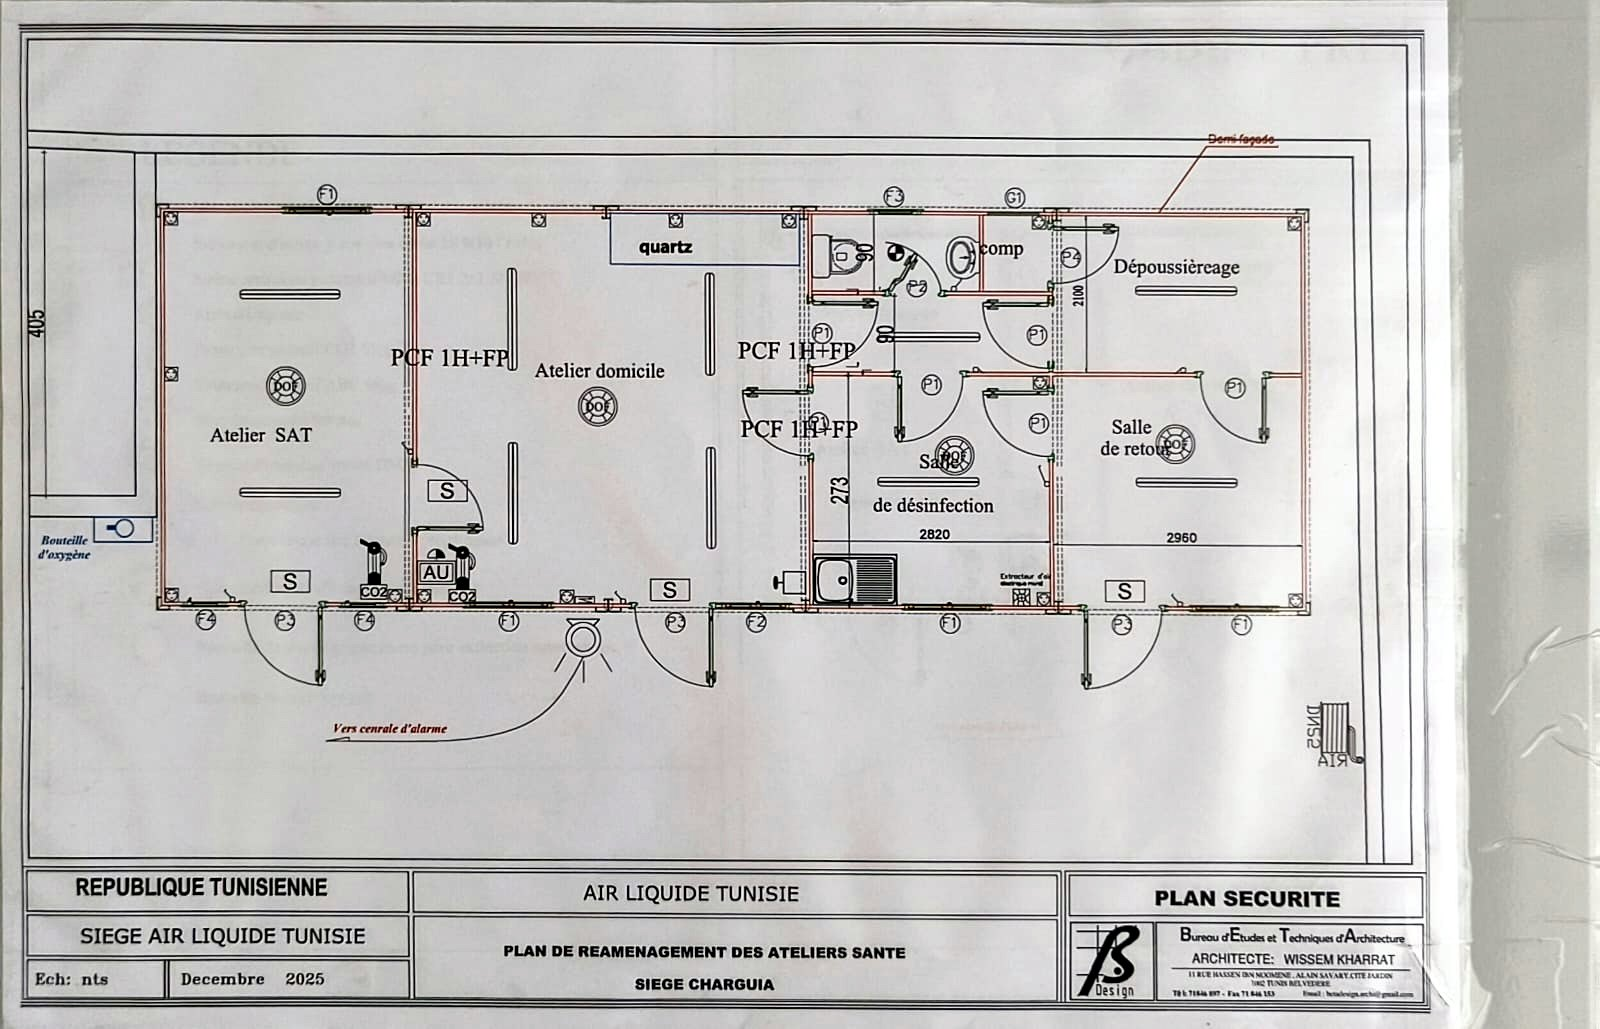
\includegraphics[width=15.5cm,height=11.0cm,keepaspectratio]{plan_ateliers_sante.jpg}
\caption{Plan de réaménagement des ateliers santé, site de Charguia (Air Liquide Tunisie, décembre 2025)}
\end{figure}

\begin{figure}[!htb]
\centering
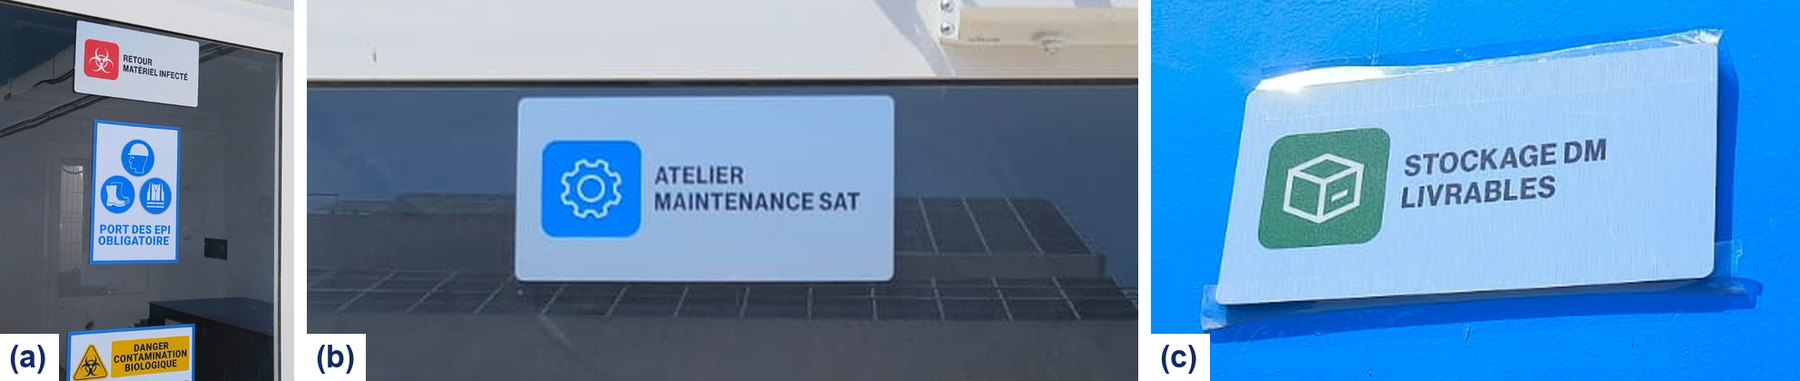
\includegraphics[width=15.5cm,height=6.5cm,keepaspectratio]{signaletique_zones.jpg}
\caption{Signalétique des zones : (a) retour du matériel infecté, (b) atelier de maintenance, (c) stockage des dispositifs médicaux livrables}
\end{figure}

\Needspace{16\baselineskip}
\section{Cadre du stage}

{\small\setstretch{1.05}\renewcommand{\arraystretch}{1.3}\arrayrulecolor{ALtexte}
\begin{longtable}{|>{\raggedright\arraybackslash}p{4.57cm}|>{\raggedright\arraybackslash}p{10.04cm}|}
\caption{Cadre du stage}\\
\hline
\rowcolor{ALbleu} \sffamily\bfseries\color{white} Élément & \sffamily\bfseries\color{white} Information \\ \hline
\endfirsthead
\caption[]{Cadre du stage (suite)}\\
\hline
\rowcolor{ALbleu} \sffamily\bfseries\color{white} Élément & \sffamily\bfseries\color{white} Information \\ \hline
\endhead
Période & du 1\textsuperscript{er} juillet au 1\textsuperscript{er} août 2026 \\ \hline
\rowcolor{ALgris} Entreprise & Air Liquide Tunisie \\ \hline
Service & Maintenance (maintenance biomédicale) \\ \hline
\rowcolor{ALgris} Encadrant professionnel & M. Marouane Hassan, responsable génie biomédical \\ \hline
Équipe d'accueil & Techniciens de l'atelier, dont Fares et Maher \\ \hline
\rowcolor{ALgris} Sujet & Conception et réalisation d'une application de gestion de la maintenance (AirLiquide GMAO+) \\ \hline
\end{longtable}
}


\chapter{Contexte et objectifs du stage}

\section{Contexte du stage}

Le service reçoit chaque jour des appareils à contrôler, réparer ou remettre en état. Chaque appareil suit un parcours défini : retour et réception, désinfection, diagnostic, réparation, contrôle qualité, stock livrable puis livraison. L'enjeu est double : garantir la \textbf{sécurité} (un appareil ne doit pas repartir sans désinfection ni contrôle) et conserver l'\textbf{historique} de chaque appareil.

Les interventions portent sur des composants variés. Sur les concentrateurs d'oxygène, il s'agit notamment du compresseur, des électrovannes, des cartes électroniques et des colonnes à tamis moléculaire ; sur les appareils de ventilation, de l'écran tactile, des cartes électroniques, de la turbine et de la batterie. Ces composants alimentent le catalogue de pannes de l'application.

\begin{figure}[!htb]
\centering
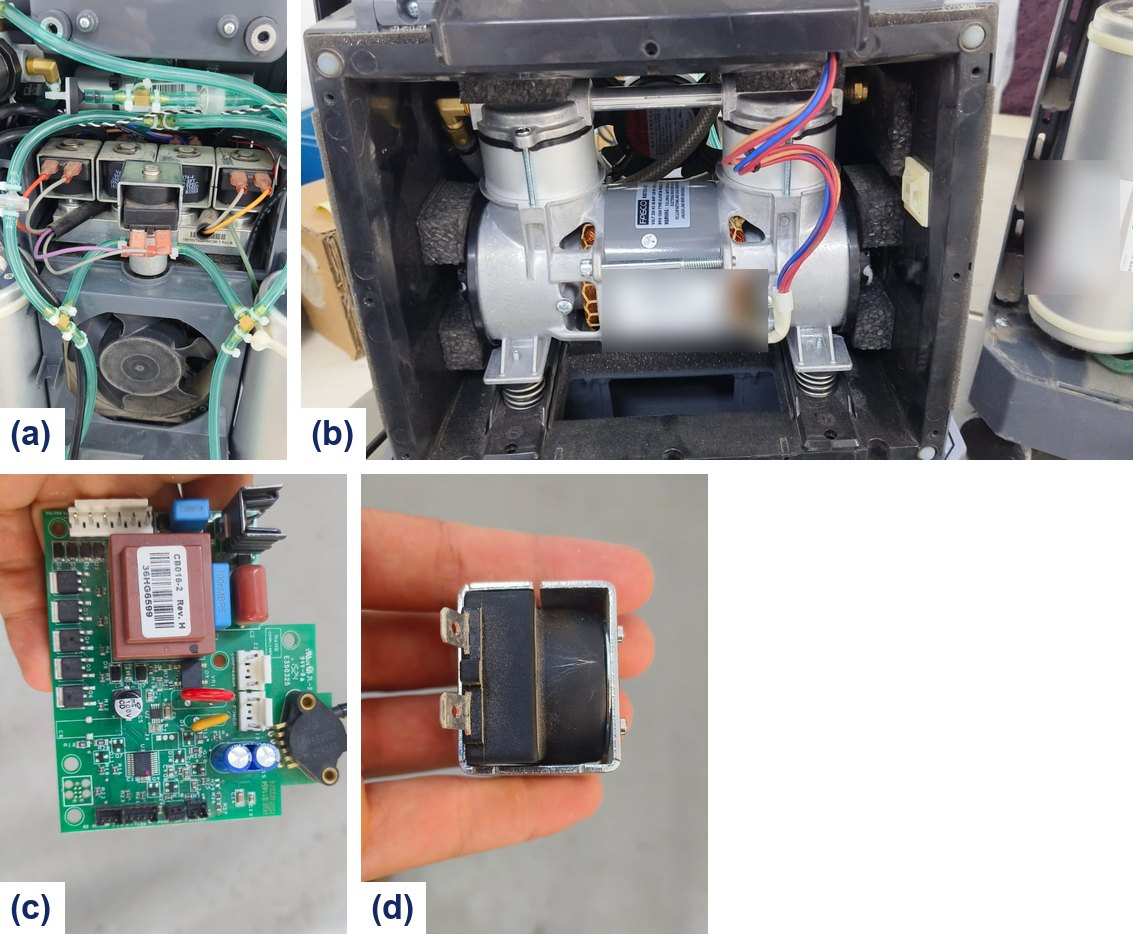
\includegraphics[width=14.0cm,height=12.0cm,keepaspectratio]{concentrateur_composants.jpg}
\caption{Composants d'un concentrateur d'oxygène : (a) vue interne, (b) compresseur, (c) carte électronique, (d) bobine d'électrovanne (étiquettes de série floutées)}
\end{figure}

\begin{figure}[!htb]
\centering
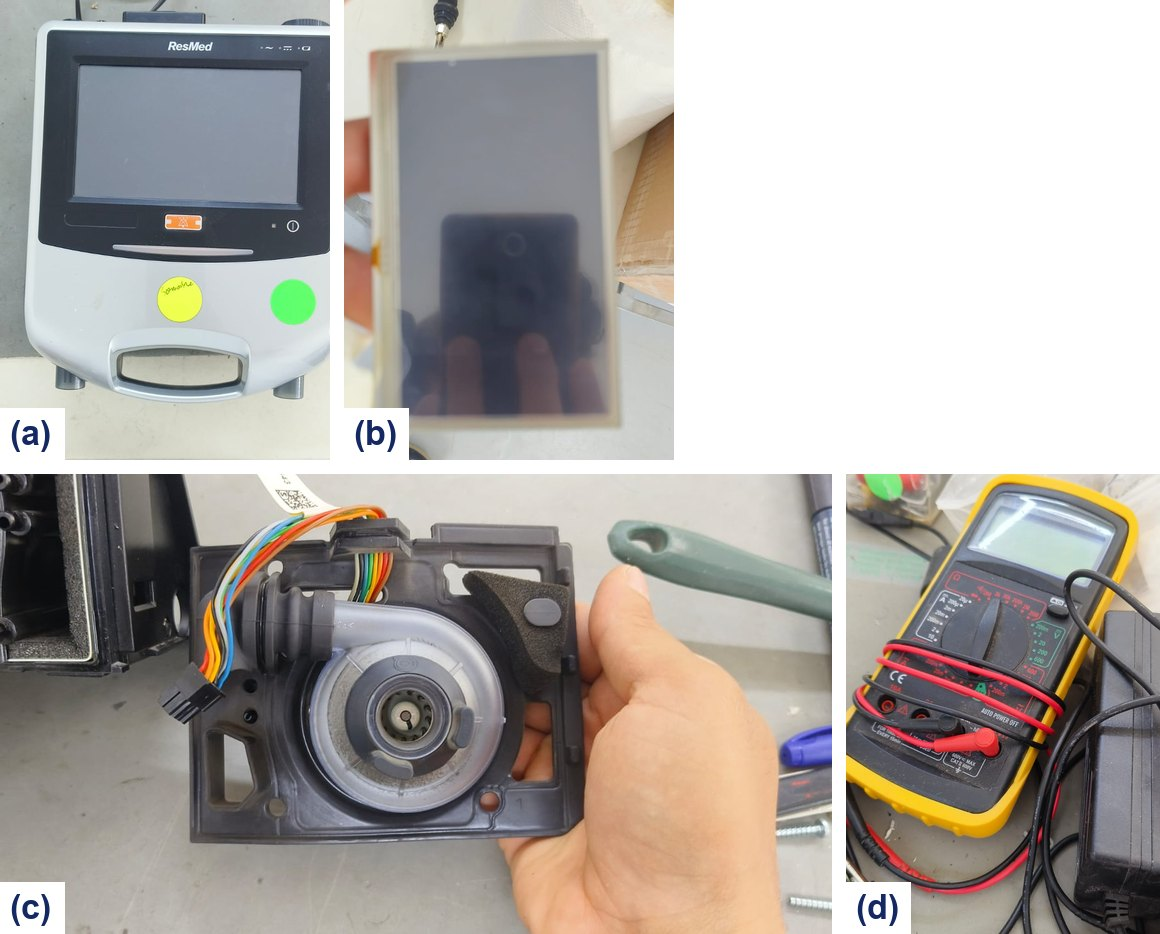
\includegraphics[width=14.0cm,height=12.0cm,keepaspectratio]{ventilation_composants.jpg}
\caption{Appareil de ventilation et composants : (a) appareil à écran tactile, (b) dalle tactile démontée, (c) turbine, (d) multimètre utilisé pour les contrôles}
\end{figure}

\section{Analyse de l'existant}

Trois supports étaient utilisés pour suivre l'activité. Par ailleurs, un progiciel de gestion (Microsoft Dynamics NAV) a été observé au poste de travail, utilisé pour les ordres de transfert ; le suivi technique des appareils restait en dehors de cet outil.

\subsection{Le journal de maintenance papier}

Un registre imprimé, intitulé \og{}Journal de maintenance des équipements O2, VNI, CPAP et respirateur\fg{} (référence 404, révision 1, propriétaire Air Liquide Tunisie), est rempli à la main pendant la journée sur un porte-bloc, une ligne par appareil. La figure suivante montre le registre le 14 juillet 2026.

\Needspace{22\baselineskip}
{\small\setstretch{1.05}\renewcommand{\arraystretch}{1.3}\arrayrulecolor{ALtexte}
\begin{longtable}{|>{\raggedright\arraybackslash}p{4.57cm}|>{\raggedright\arraybackslash}p{10.04cm}|}
\caption{Colonnes du journal de maintenance papier}\\
\hline
\rowcolor{ALbleu} \sffamily\bfseries\color{white} Colonne du registre & \sffamily\bfseries\color{white} Information notée \\ \hline
\endfirsthead
\caption[]{Colonnes du journal de maintenance papier (suite)}\\
\hline
\rowcolor{ALbleu} \sffamily\bfseries\color{white} Colonne du registre & \sffamily\bfseries\color{white} Information notée \\ \hline
\endhead
Année, Mois & Date de l'intervention \\ \hline
\rowcolor{ALgris} Équip. / type & Type d'équipement \\ \hline
N° série & Numéro de série de l'appareil \\ \hline
\rowcolor{ALgris} C.H & Compteur horaire de l'appareil \\ \hline
Pureté & Pureté de l'oxygène produit (concentrateurs) \\ \hline
\rowcolor{ALgris} Débit / pression & Mesures de débit ou de pression \\ \hline
Alarme sonore & Fonctionnement de l'alarme \\ \hline
\rowcolor{ALgris} Pannes & Pannes constatées \\ \hline
Doc de sortie PR & Document de sortie des pièces utilisées \\ \hline
\rowcolor{ALgris} Technicien & Technicien intervenant \\ \hline
Date sortie & Date de sortie de l'appareil \\ \hline
\end{longtable}
}

\begin{figure}[!htb]
\centering
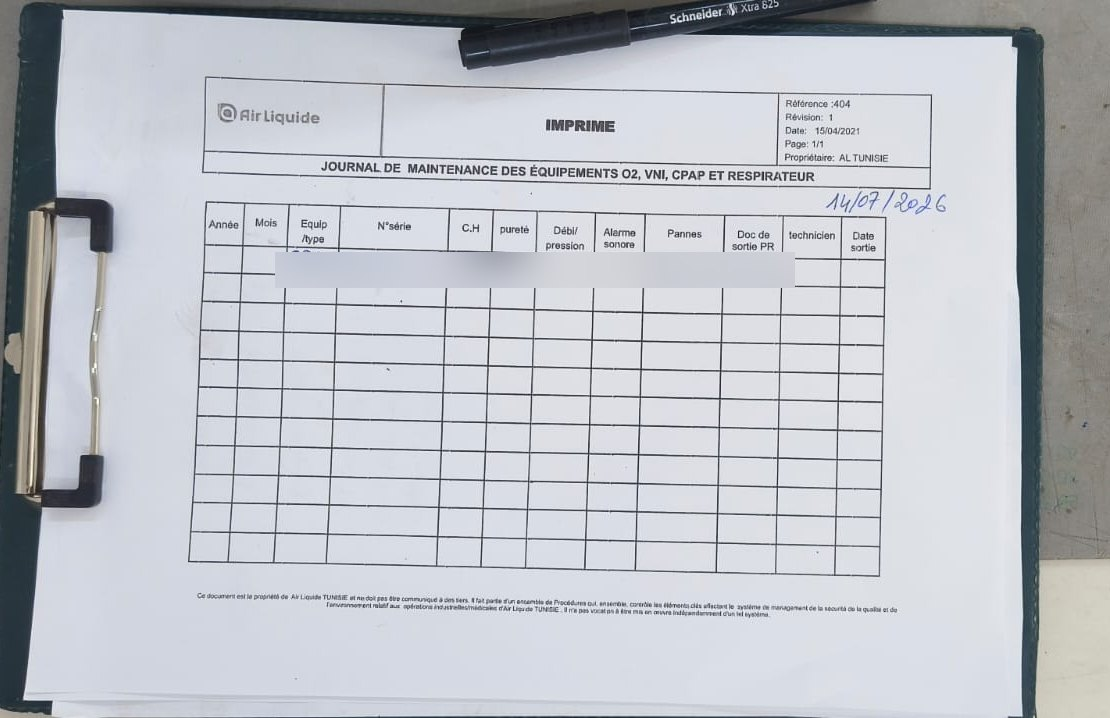
\includegraphics[width=13.5cm,height=10.0cm,keepaspectratio]{journal_papier.jpg}
\caption{Journal de maintenance papier du service (ligne manuscrite floutée)}
\end{figure}

\subsection{Le classeur Google Sheets \og{}GMAO v1\fg{}}

En fin de journée, les informations du papier étaient reportées dans un classeur Google Sheets. Il comporte plusieurs onglets, dont \textbf{RETURNS} (retours d'appareils), \textbf{DISINFECTION} (opérateur, statut, notes), \textbf{MAINTENANCE\_\allowbreak{}JOURNAL} (type de service, pièces, catégorie, propriété, heures de fonctionnement, pureté, dates de service), \textbf{LISTS}, \textbf{PM\_\allowbreak{}LOG} et \textbf{CM\_\allowbreak{}LOG}.

\begin{figure}[!htb]
\centering
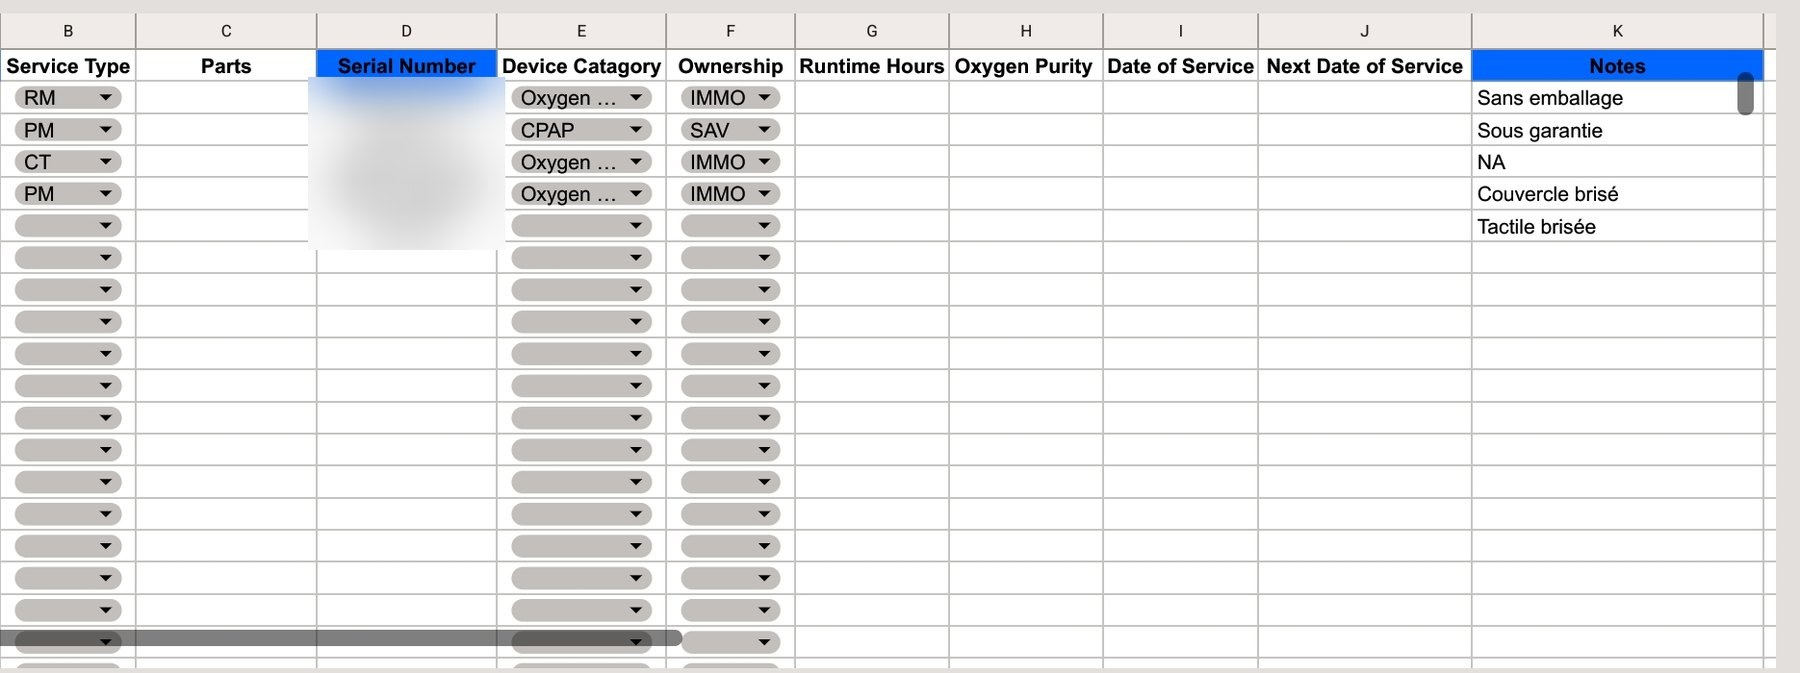
\includegraphics[width=15.5cm,height=7.0cm,keepaspectratio]{classeur_journal.jpg}
\caption{Onglet MAINTENANCE\_\allowbreak{}JOURNAL du classeur (numéros de série floutés)}
\end{figure}

\subsection{Le questionnaire de retour}

Avant l'arrivée d'un appareil, un questionnaire en ligne annonce le retour. Il recueille le numéro de série, l'état visuel (bon état, dégâts mineurs, réparation nécessaire, risque biologique), les accessoires manquants, des notes, un identifiant de retour et le statut biologique (normal, contamination importante, inconnu). Ses réponses alimentent l'onglet RETURNS du classeur.

\begin{figure}[!htb]
\centering
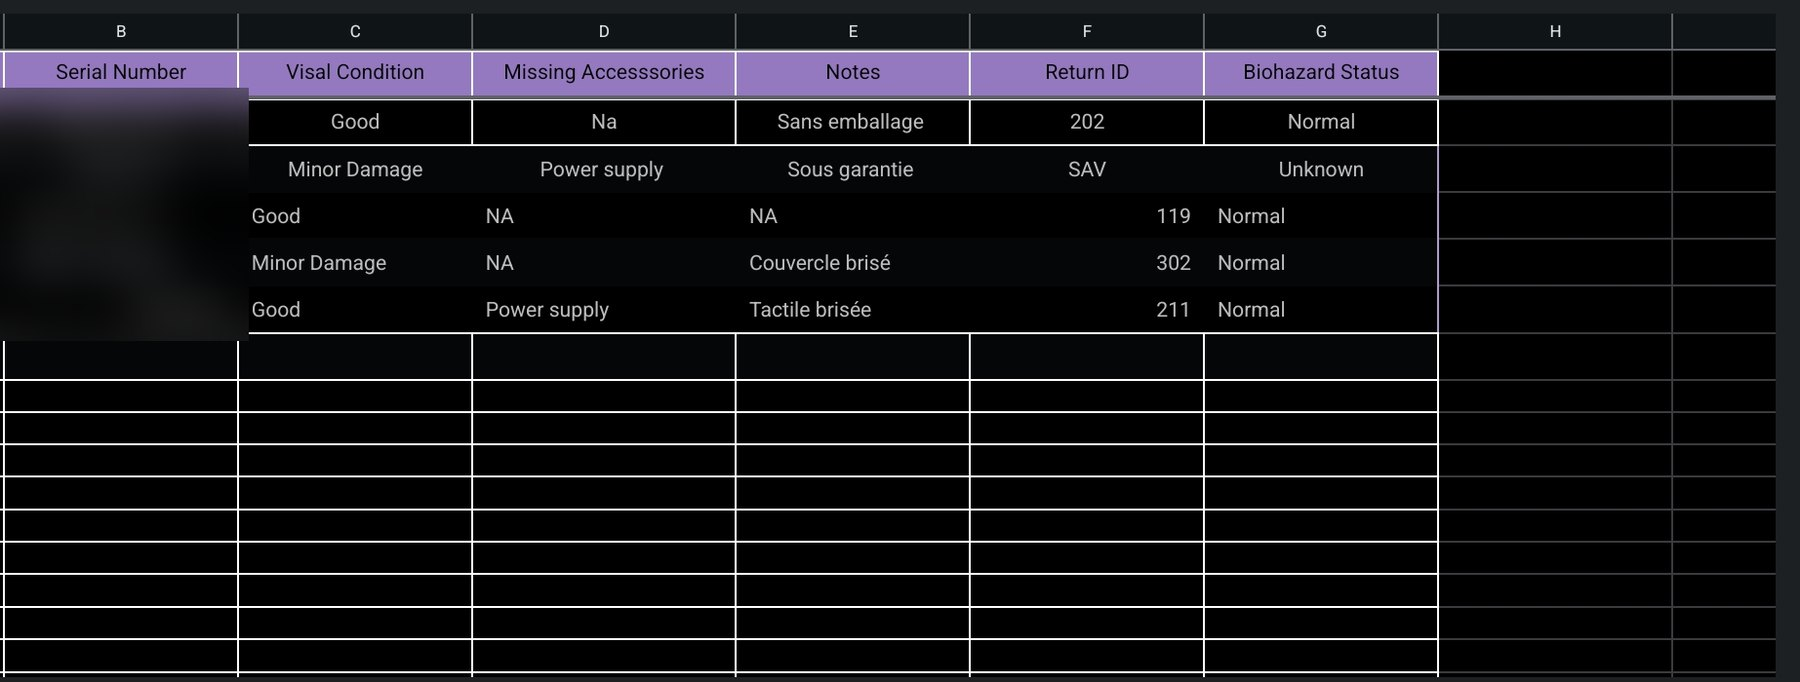
\includegraphics[width=15.5cm,height=6.5cm,keepaspectratio]{classeur_retours.jpg}
\caption{Onglet RETURNS : réponses au questionnaire de retour (numéros de série floutés)}
\end{figure}

\section{Problématique}

Ces supports présentent plusieurs limites, relevées dans le cahier des charges du projet : recherche lente des équipements, double saisie des informations, difficulté de suivre l'état des machines, absence de traçabilité complète et absence d'indicateurs de performance. La question centrale du stage est la suivante : \textbf{comment centraliser le suivi des appareils de leur retour à leur livraison, avec une traçabilité fiable et une saisie rapide pour les techniciens ?}

\section{Objectifs du stage}

\Needspace{22\baselineskip}
{\small\setstretch{1.05}\renewcommand{\arraystretch}{1.3}\arrayrulecolor{ALtexte}
\begin{longtable}{|>{\raggedright\arraybackslash}p{4.90cm}|>{\raggedright\arraybackslash}p{5.79cm}|>{\raggedright\arraybackslash}p{3.56cm}|}
\caption{Objectifs du stage et état de réalisation}\\
\hline
\rowcolor{ALbleu} \sffamily\bfseries\color{white} Objectif & \sffamily\bfseries\color{white} Critère de vérification & \sffamily\bfseries\color{white} Statut \\ \hline
\endfirsthead
\caption[]{Objectifs du stage et état de réalisation (suite)}\\
\hline
\rowcolor{ALbleu} \sffamily\bfseries\color{white} Objectif & \sffamily\bfseries\color{white} Critère de vérification & \sffamily\bfseries\color{white} Statut \\ \hline
\endhead
Enregistrer rapidement les retours & Formulaire de réception, reprise du questionnaire de retour & Réalisé \\ \hline
\rowcolor{ALgris} Une fiche de vie unique par appareil & Test : un appareil qui revient garde la même fiche & Réalisé, testé \\ \hline
Suivre chaque étape du cycle de maintenance & Workflow à 7 statuts, historique horodaté & Réalisé, testé \\ \hline
\rowcolor{ALgris} Empêcher les transitions incohérentes & Tests des règles de transition et des prérequis & Réalisé, testé \\ \hline
Enregistrer diagnostics, pannes, réparations, pièces & Catalogues et formulaires d'étape & Réalisé, testé \\ \hline
\rowcolor{ALgris} Contrôle qualité avec checklist & Checklist de 7 points, mesures & Réalisé, testé \\ \hline
Gérer le stock des appareils réparés & Mouvements d'entrée et de sortie & Réalisé, testé \\ \hline
\rowcolor{ALgris} Fournir tableau de bord et statistiques & Indicateurs et exports & Réalisé (tableau de bord, exports CSV) \\ \hline
Rapports PDF & Mentionnés au cahier des charges & Non réalisé (export CSV seulement) \\ \hline
\rowcolor{ALgris} Temps de saisie inférieur à une minute & Exigence du cahier des charges & Non mesuré \\ \hline
\end{longtable}
}

\section{Intérêt du stage dans ce contexte}

Le projet répond à un besoin réel du service. Il a permis de mettre en pratique la démarche complète d'un projet logiciel appliqué à la santé : recueil du besoin auprès des utilisateurs, conception, développement, tests et validation. Il se rattache directement à la formation TTIS, qui associe systèmes d'information et dispositifs médicaux.


\chapter{Travaux réalisés}

\section{Démarche et organisation du travail}

Le travail a suivi une démarche en trois temps : (1) documenter le besoin avant d'écrire du code, (2) concevoir l'architecture et le modèle de données, (3) développer fonctionnalité par fonctionnalité, en testant chaque règle métier.

\begin{itemize}
  \item \textbf{Documentation préalable} : vision, cahier des charges, objectifs, workflow, cas d'utilisation, architecture et base de données (documents Markdown versionnés dans le dépôt).
  \item \textbf{Gestion de version Git} : branche \texttt{main} stable, branche \texttt{develop} d'intégration, branches de fonctionnalité et messages de commit normalisés (Conventional Commits). Le dépôt compte 31 commits.
  \item \textbf{Développement piloté par les règles métier} : chaque règle (transition, unicité, permission) est couverte par un test automatisé.
\end{itemize}

Le déroulement du projet est reconstitué à partir des observations du stage et de l'historique du dépôt Git.

\Needspace{7\baselineskip}

{\small\setstretch{1.05}\renewcommand{\arraystretch}{1.3}\arrayrulecolor{ALtexte}
\begin{longtable}{|>{\raggedright\arraybackslash}p{4.11cm}|>{\raggedright\arraybackslash}p{10.50cm}|}
\caption{Déroulement du projet}\\
\hline
\rowcolor{ALbleu} \sffamily\bfseries\color{white} Période & \sffamily\bfseries\color{white} Activité \\ \hline
\endfirsthead
\caption[]{Déroulement du projet (suite)}\\
\hline
\rowcolor{ALbleu} \sffamily\bfseries\color{white} Période & \sffamily\bfseries\color{white} Activité \\ \hline
\endhead
1\textsuperscript{er} juillet – 1\textsuperscript{er} août 2026 (stage) & Immersion au service Maintenance : observation du circuit retour, désinfection, atelier et stockage ; échanges avec le responsable et les techniciens ; recueil du besoin à partir du journal papier (entrée du 14 juillet 2026), du classeur Google Sheets et du questionnaire de retour \\ \hline
\rowcolor{ALgris} 15 et 16 juillet 2026 & Rédaction de la documentation de conception (vision, cahier des charges, workflow, cas d'utilisation, architecture, base de données), structure du dépôt, projet Django \\ \hline
Octobre 2026 (14, 27 et 28) & Réalisation et consolidation de l'application : authentification, workflow complet, questionnaire de retour, journal, interface, tests et documentation \\ \hline
\end{longtable}
}

\subsection{Outils d'assistance utilisés}

Conformément à une démarche transparente, il est précisé que des assistants d'intelligence artificielle ont été utilisés comme outils de travail : un assistant conversationnel pour structurer la conception initiale (architecture, base de données, workflow), puis un assistant de programmation pour accélérer le développement et la rédaction des tests. L'étudiant a défini le besoin, pris les décisions de conception, relu, exécuté et validé le résultat.

\section{Analyse des besoins}

\Needspace{10\baselineskip}
\subsection{Acteurs}

{\small\setstretch{1.05}\renewcommand{\arraystretch}{1.3}\arrayrulecolor{ALtexte}
\begin{longtable}{|>{\raggedright\arraybackslash}p{3.56cm}|>{\raggedright\arraybackslash}p{4.00cm}|>{\raggedright\arraybackslash}p{6.67cm}|}
\caption{Acteurs et droits}\\
\hline
\rowcolor{ALbleu} \sffamily\bfseries\color{white} Acteur & \sffamily\bfseries\color{white} Rôle dans l'application & \sffamily\bfseries\color{white} Droits principaux \\ \hline
\endfirsthead
\caption[]{Acteurs et droits (suite)}\\
\hline
\rowcolor{ALbleu} \sffamily\bfseries\color{white} Acteur & \sffamily\bfseries\color{white} Rôle dans l'application & \sffamily\bfseries\color{white} Droits principaux \\ \hline
\endhead
Technicien de maintenance & Utilisateur principal de l'atelier & Enregistrer les retours, réaliser et valider chaque étape, consulter les fiches de vie et le journal \\ \hline
\rowcolor{ALgris} Responsable SAV & Supervision et administration & Tous les droits du technicien, plus : gestion des utilisateurs et des catalogues, rapports et exports, retour arrière d'un statut avec justification \\ \hline
\end{longtable}
}

\begin{figure}[p]
\centering
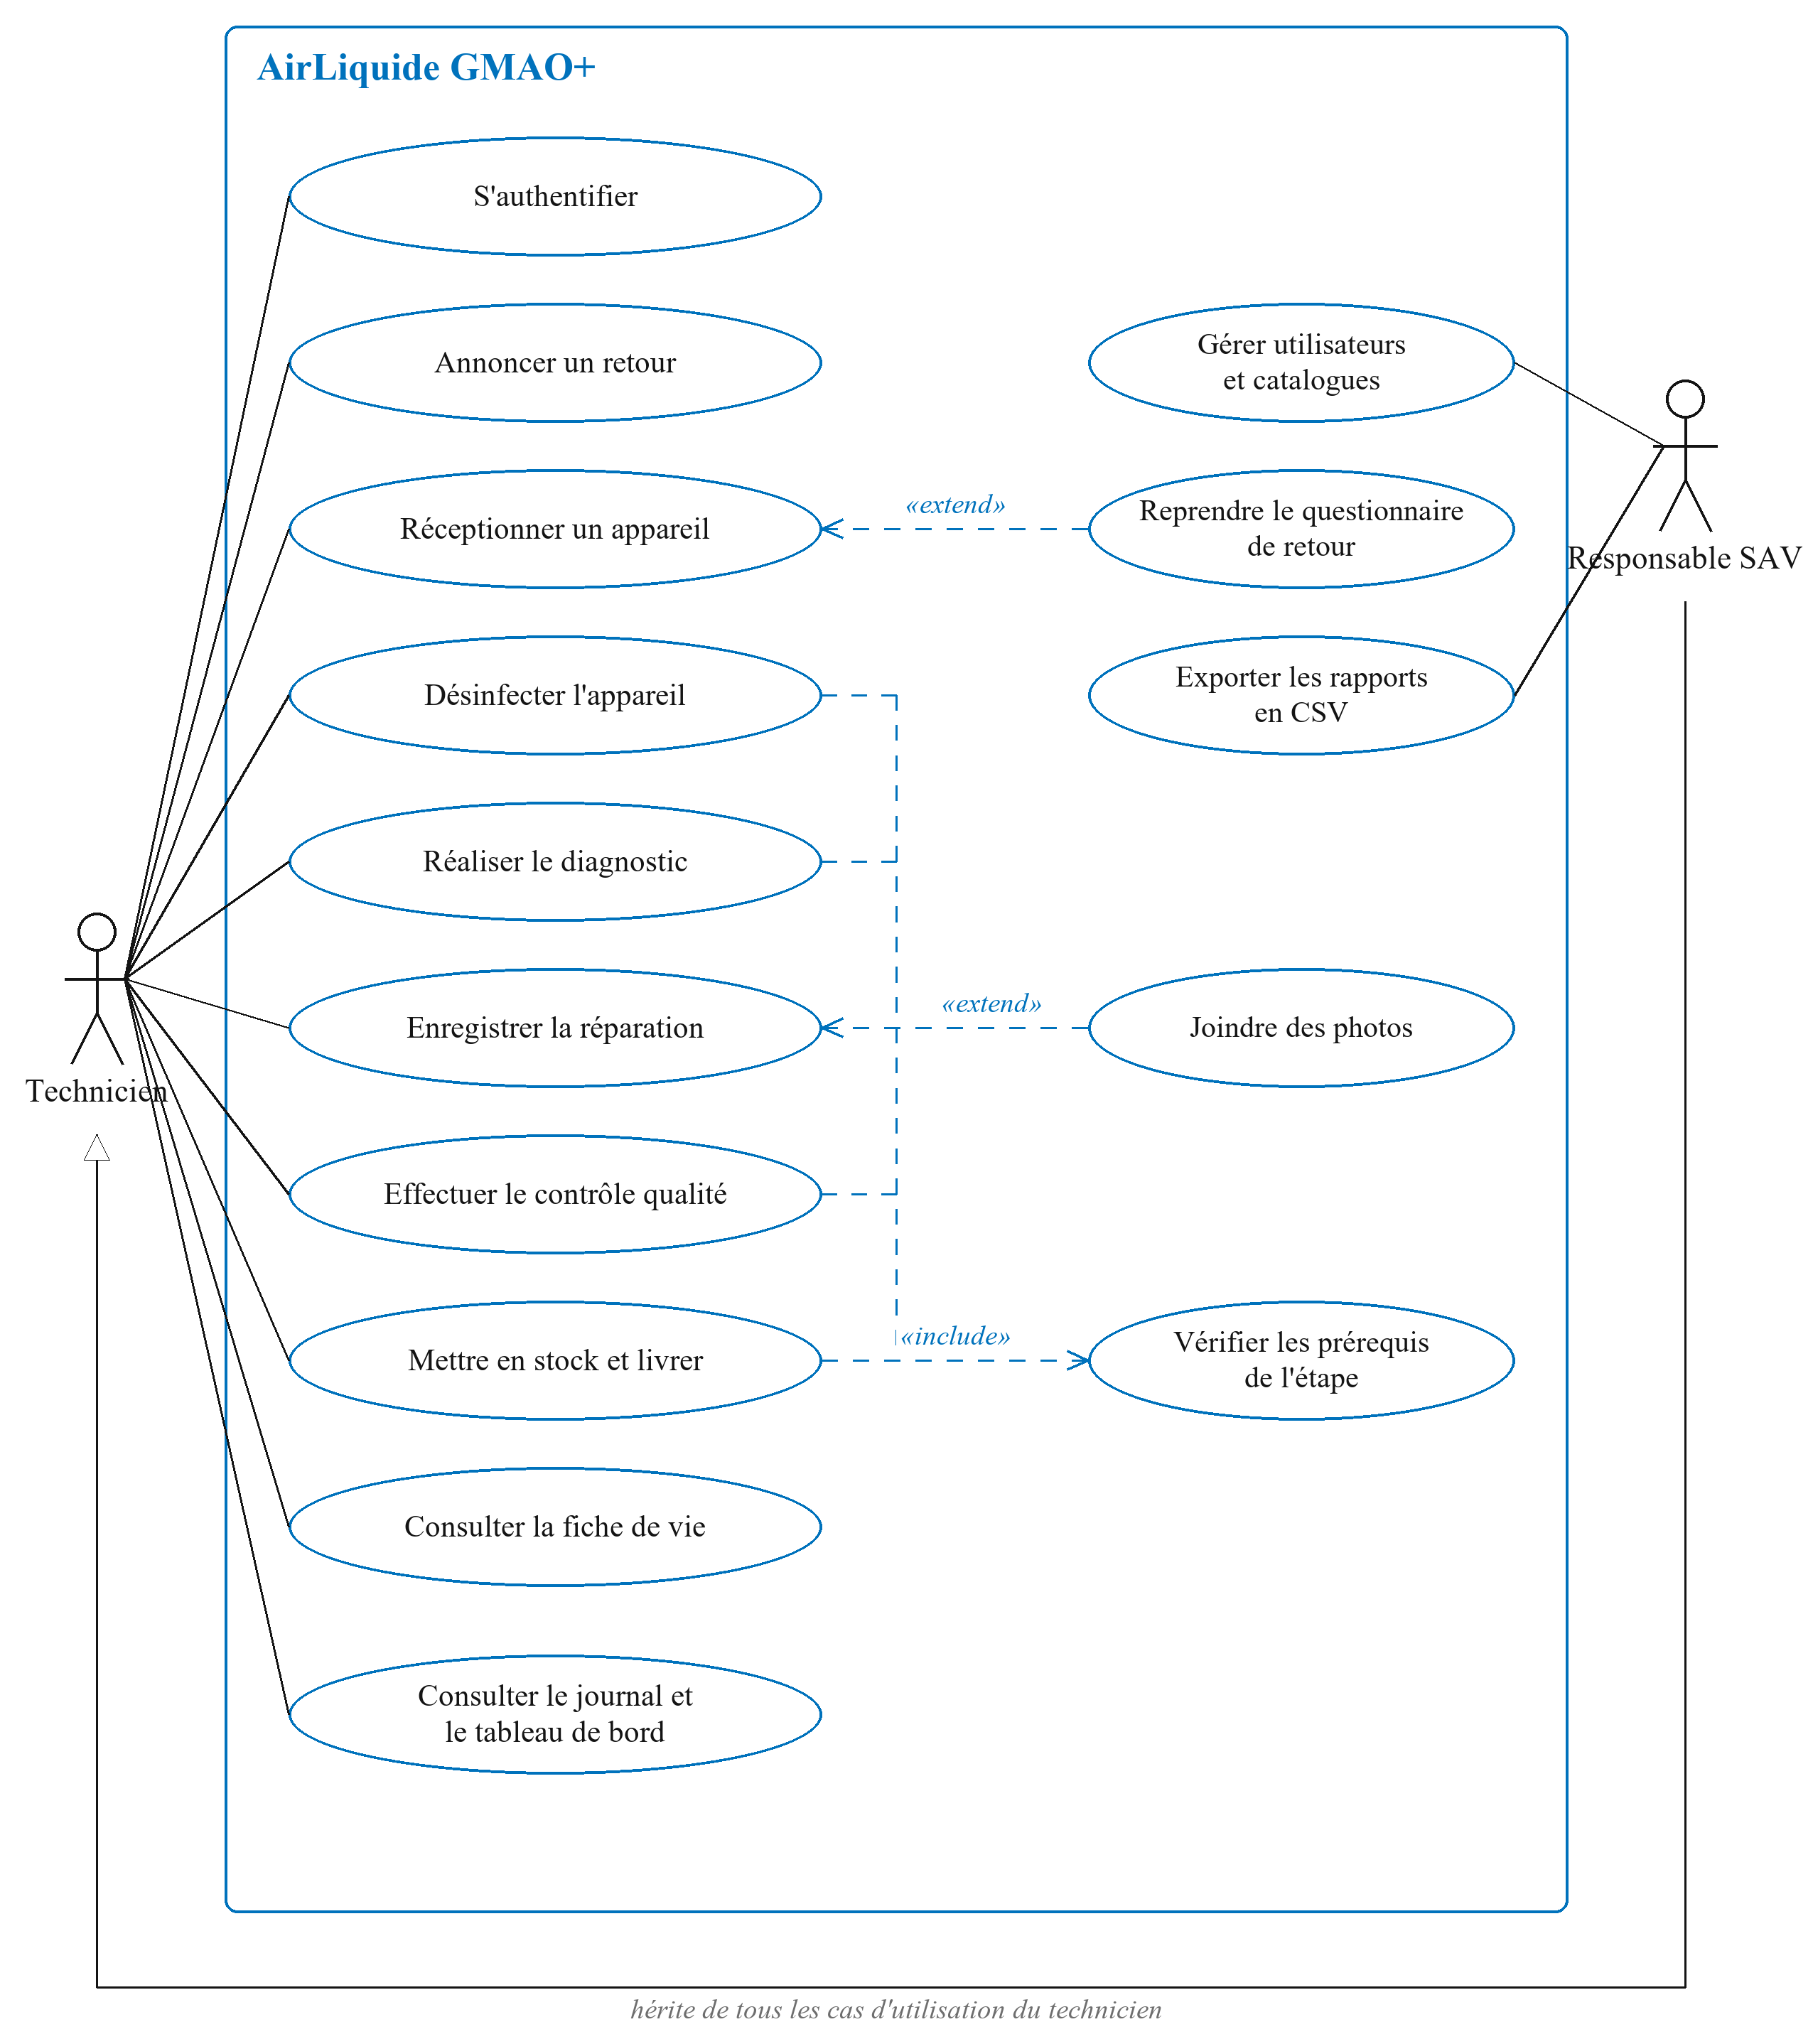
\includegraphics[width=15.5cm,height=18.5cm,keepaspectratio]{uml_cas_utilisation.png}
\caption{Diagramme de cas d'utilisation}
\end{figure}

Le Responsable SAV hérite de tous les cas d'utilisation du technicien et dispose en plus de la gestion des utilisateurs et des catalogues et de l'export des rapports. Chaque étape du workflow inclut la vérification de ses prérequis.

\subsection{Besoins fonctionnels}

\begin{itemize}
  \item annoncer un retour avant l'arrivée de l'appareil, puis le réceptionner ;
  \item retrouver un appareil par son numéro de série et consulter sa fiche de vie ;
  \item enregistrer la désinfection, le diagnostic (pannes d'un catalogue), la réparation (pièces, durée), le contrôle qualité (checklist et mesures), l'entrée en stock et la livraison ;
  \item joindre des photos aux dossiers ;
  \item consulter un tableau de bord et un journal de maintenance équivalent au registre papier ;
  \item exporter les données (CSV).
\end{itemize}

\subsection{Besoins non fonctionnels}

\begin{itemize}
  \item \textbf{Traçabilité} : chaque changement de statut conserve la date, l'heure et l'utilisateur ; l'historique ne peut être ni modifié ni supprimé ;
  \item \textbf{Sécurité} : authentification, permissions par rôle, validation des entrées côté serveur, protection des fichiers téléversés ;
  \item \textbf{Ergonomie} : interface en français, utilisable sur ordinateur et tablette, parcours courts pour les techniciens ;
  \item \textbf{Maintenabilité} : code modulaire, logique métier séparée des vues, tests automatisés.
\end{itemize}

\section{Conception}

Les diagrammes de cette section suivent la notation UML. Ils ont été dessinés pour ce rapport ; leurs sources textuelles équivalentes (PlantUML et Mermaid), versionnées avec le projet, se trouvent dans le dossier \texttt{docs/\allowbreak{}diagrams/\allowbreak{}}.

\subsection{Le workflow d'un appareil}

Le cycle de vie d'un appareil est modélisé par sept statuts successifs. Un dossier ne peut avancer que d'une étape à la fois, et seulement si l'étape correspondante a été enregistrée.

\begin{figure}[p]
\centering
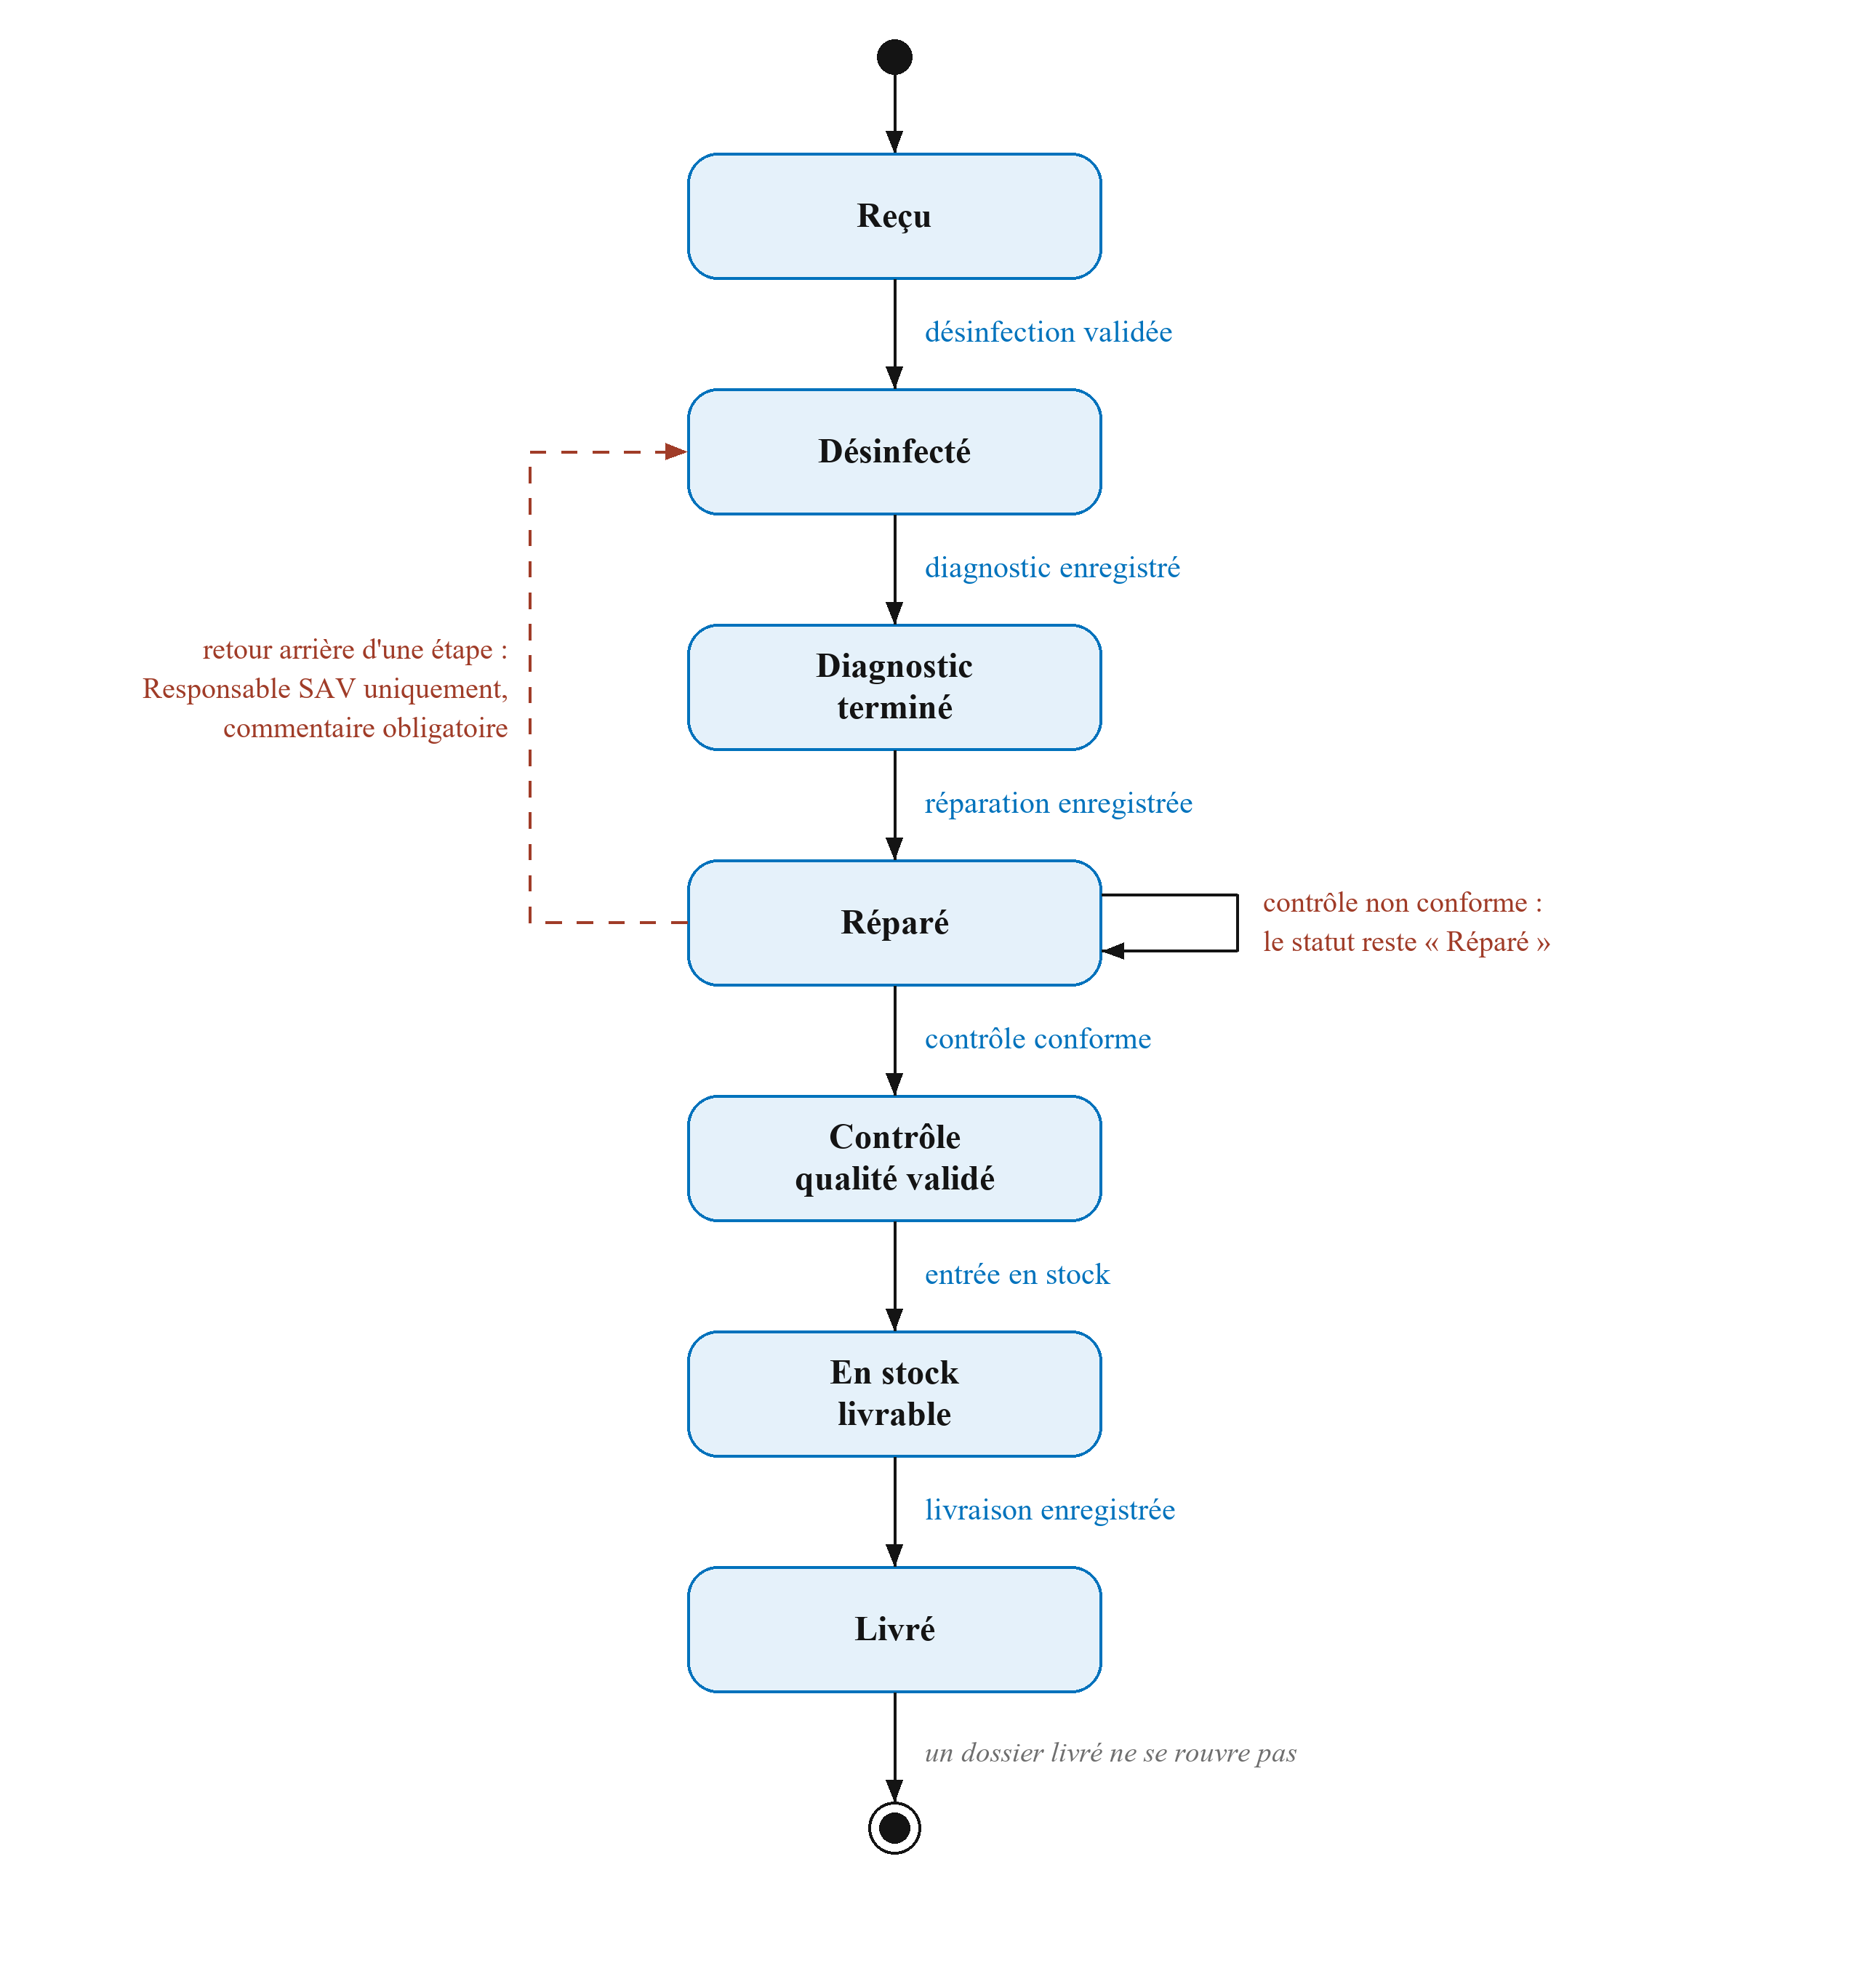
\includegraphics[width=15.5cm,height=18.5cm,keepaspectratio]{uml_etats.png}
\caption{Diagramme d'états d'un dossier SAV}
\end{figure}

\Needspace{14\baselineskip}

{\small\setstretch{1.05}\renewcommand{\arraystretch}{1.3}\arrayrulecolor{ALtexte}
\begin{longtable}{|>{\raggedright\arraybackslash}p{3.56cm}|>{\raggedright\arraybackslash}p{3.12cm}|>{\raggedright\arraybackslash}p{7.57cm}|}
\caption{Statuts du dossier SAV et prérequis}\\
\hline
\rowcolor{ALbleu} \sffamily\bfseries\color{white} Statut & \sffamily\bfseries\color{white} Étape validée & \sffamily\bfseries\color{white} Prérequis pour y accéder \\ \hline
\endfirsthead
\caption[]{Statuts du dossier SAV et prérequis (suite)}\\
\hline
\rowcolor{ALbleu} \sffamily\bfseries\color{white} Statut & \sffamily\bfseries\color{white} Étape validée & \sffamily\bfseries\color{white} Prérequis pour y accéder \\ \hline
\endhead
RECU & Réception & Appareil identifié par son numéro de série \\ \hline
\rowcolor{ALgris} DESINFECTE & Désinfection & Désinfection enregistrée et validée \\ \hline
DIAGNOSTIC\_\allowbreak{}TERMINE & Diagnostic & Diagnostic enregistré (pannes du type d'appareil) \\ \hline
\rowcolor{ALgris} REPARE & Réparation & Réparation enregistrée (début, fin, pièces) \\ \hline
QC\_\allowbreak{}VALIDE & Contrôle qualité & Dernier contrôle conforme sur les 7 points \\ \hline
\rowcolor{ALgris} EN\_\allowbreak{}STOCK & Entrée en stock & Emplacement renseigné \\ \hline
LIVRE & Livraison & Destinataire renseigné \\ \hline
\end{longtable}
}

\subsection{Règles métier}

\begin{itemize}
  \item un appareil physique possède \textbf{une seule fiche} (numéro de série normalisé) et peut avoir plusieurs retours ;
  \item un appareil ne peut avoir \textbf{qu'un seul dossier ouvert} à la fois (contrainte en base de données) ;
  \item aucun saut d'étape n'est possible ; le statut ne se modifie pas directement par l'API ;
  \item le \textbf{retour arrière} est réservé au Responsable SAV avec commentaire obligatoire, et un dossier livré ne se rouvre pas ;
  \item un contrôle qualité non conforme exige un commentaire, laisse le dossier à l'état \og{}réparé\fg{} et bloque la mise en stock ;
  \item le \textbf{risque biologique} est déduit du questionnaire : un statut \og{}inconnu\fg{} est traité comme un risque, par précaution ;
  \item les pannes d'un diagnostic doivent appartenir au type de l'appareil.
\end{itemize}

\subsection{Modèle de données}

Une décision de conception importante a été de \textbf{séparer l'appareil physique de ses retours}. La première version de la conception reposait sur une entité unique \og{}Machine\fg{} ; elle a évolué vers deux entités : l'\textbf{appareil} (fiche de vie durable, créée une seule fois) et le \textbf{dossier SAV} (un retour, avec ses étapes). Ainsi, un appareil qui revient plusieurs fois au service n'est jamais recréé.

Le modèle est présenté en deux diagrammes de classes : le premier montre le cœur (utilisateurs, appareils, retours et historique), le second les étapes rattachées à un dossier.

\begin{figure}[p]
\centering
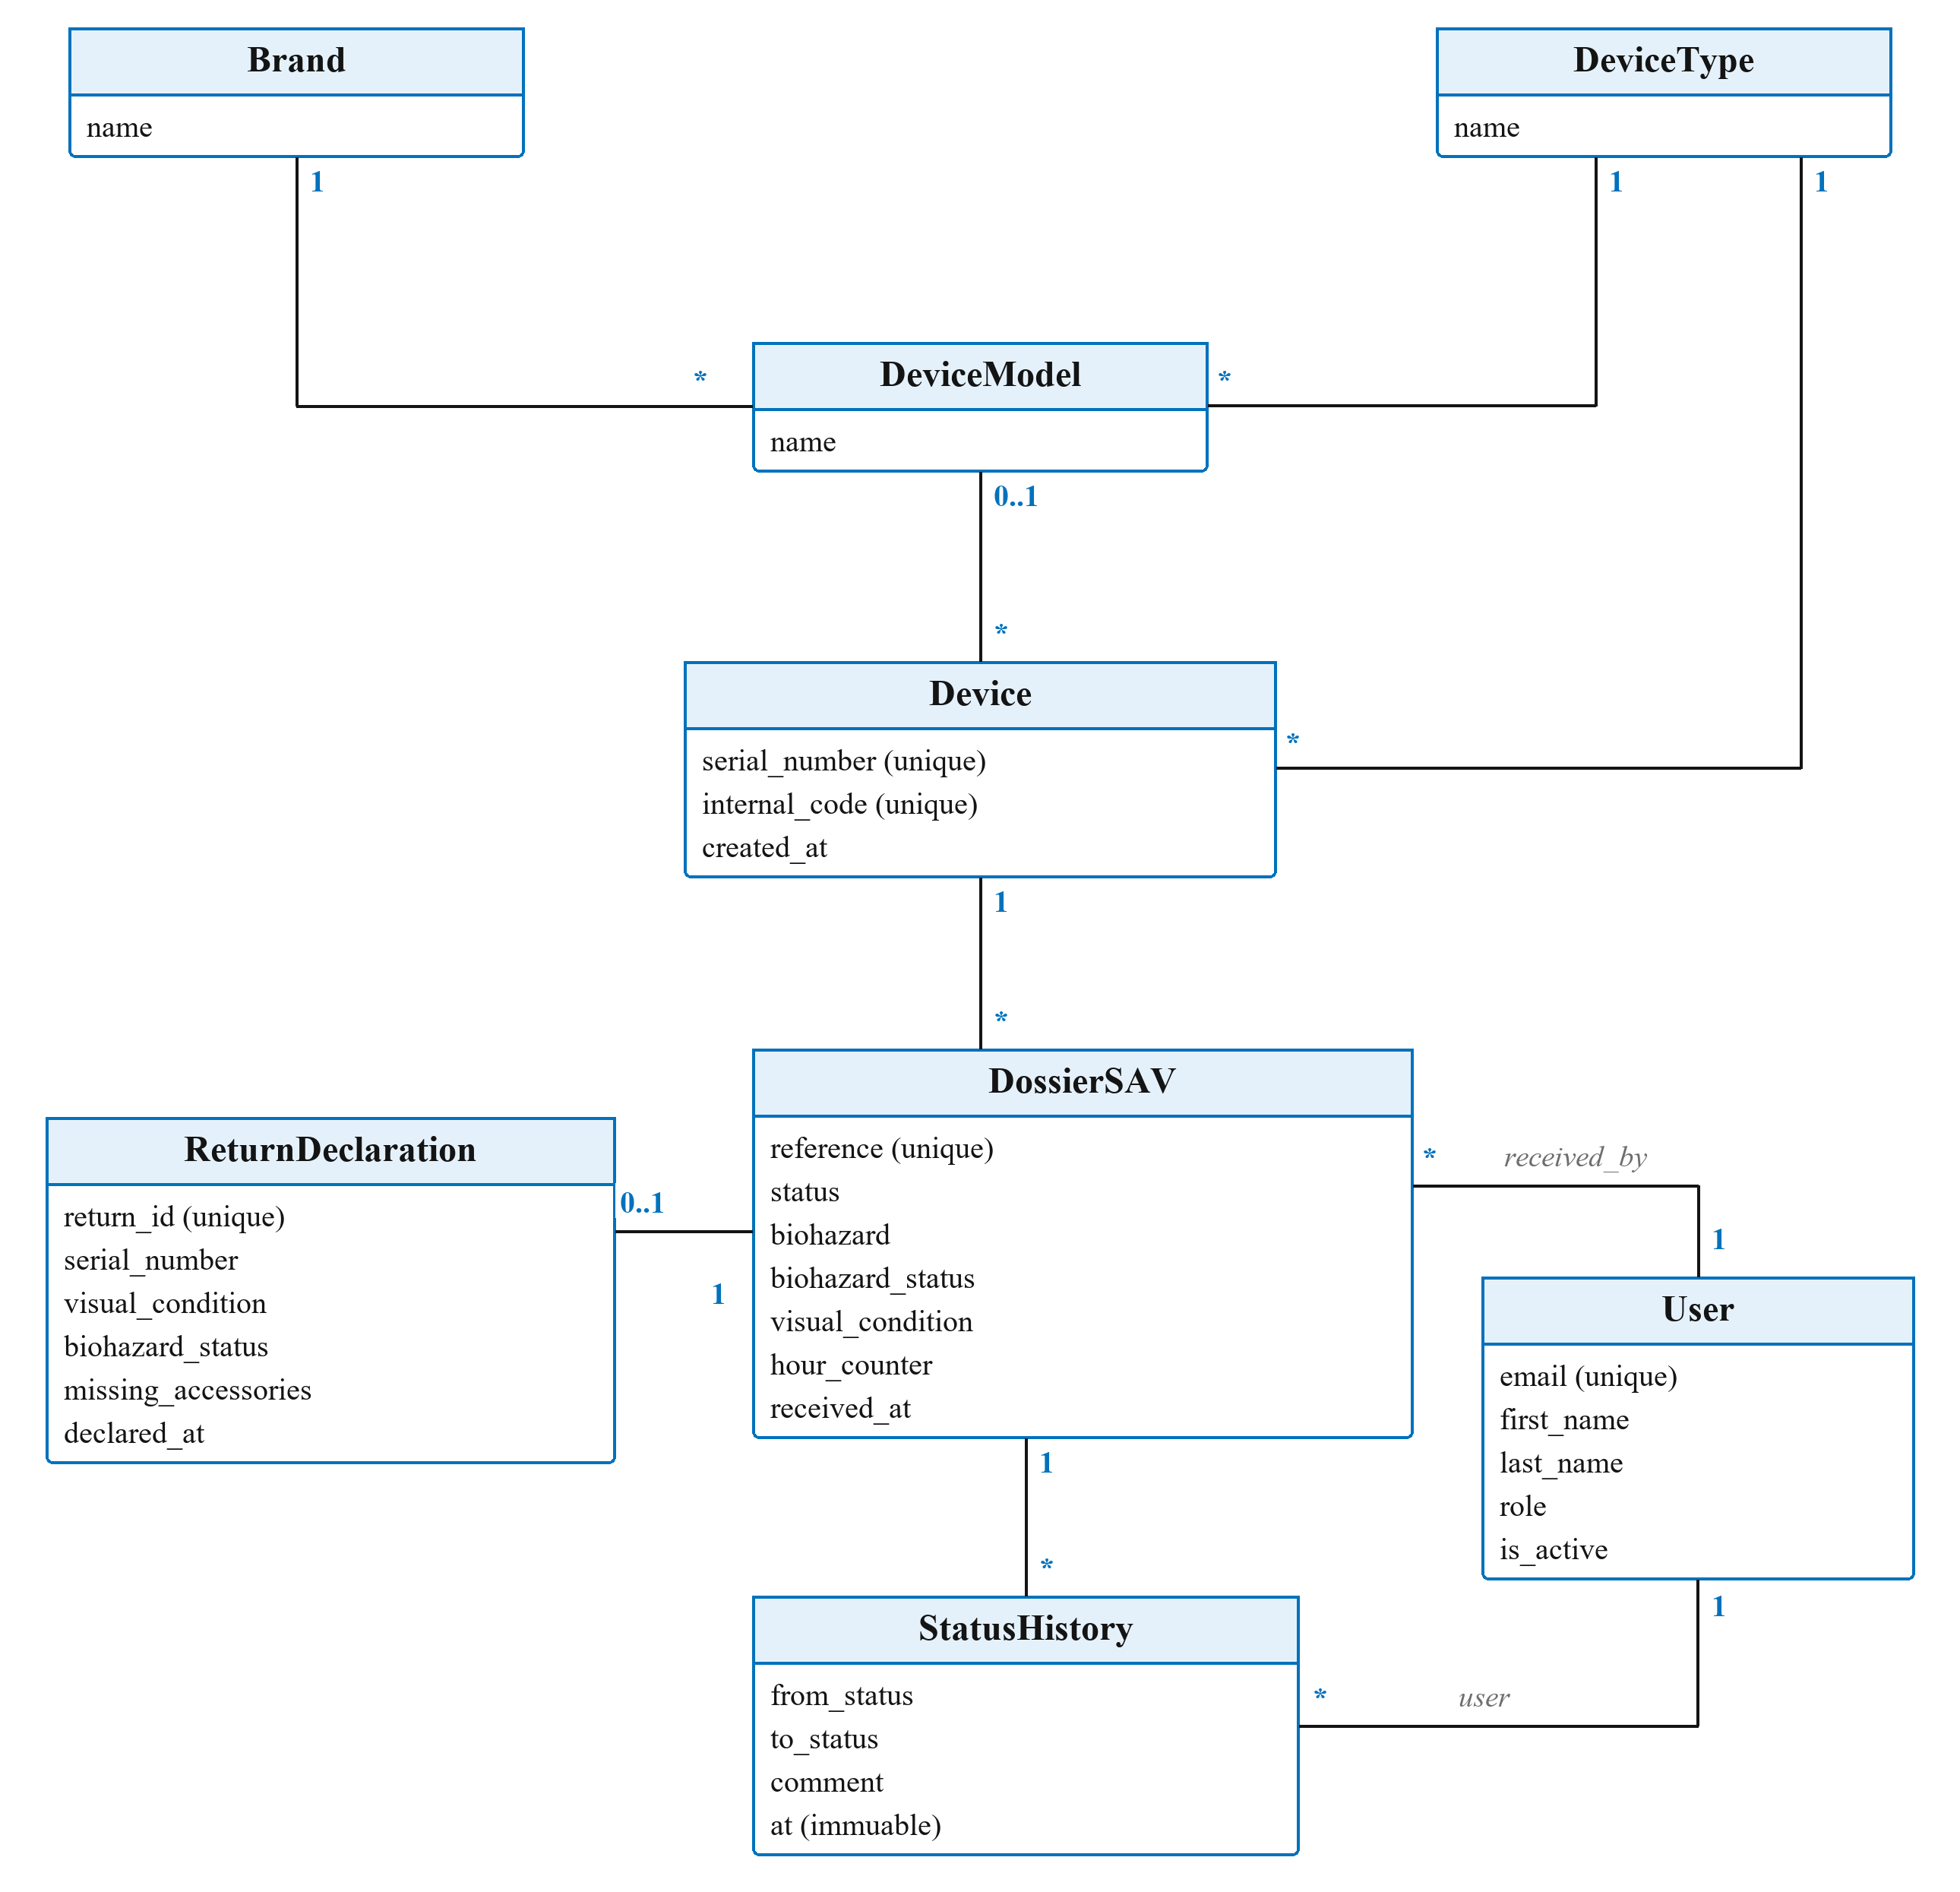
\includegraphics[width=15.5cm,height=18.5cm,keepaspectratio]{uml_classes_coeur.png}
\caption{Diagramme de classes : appareil, retour et historique}
\end{figure}

\begin{figure}[p]
\centering
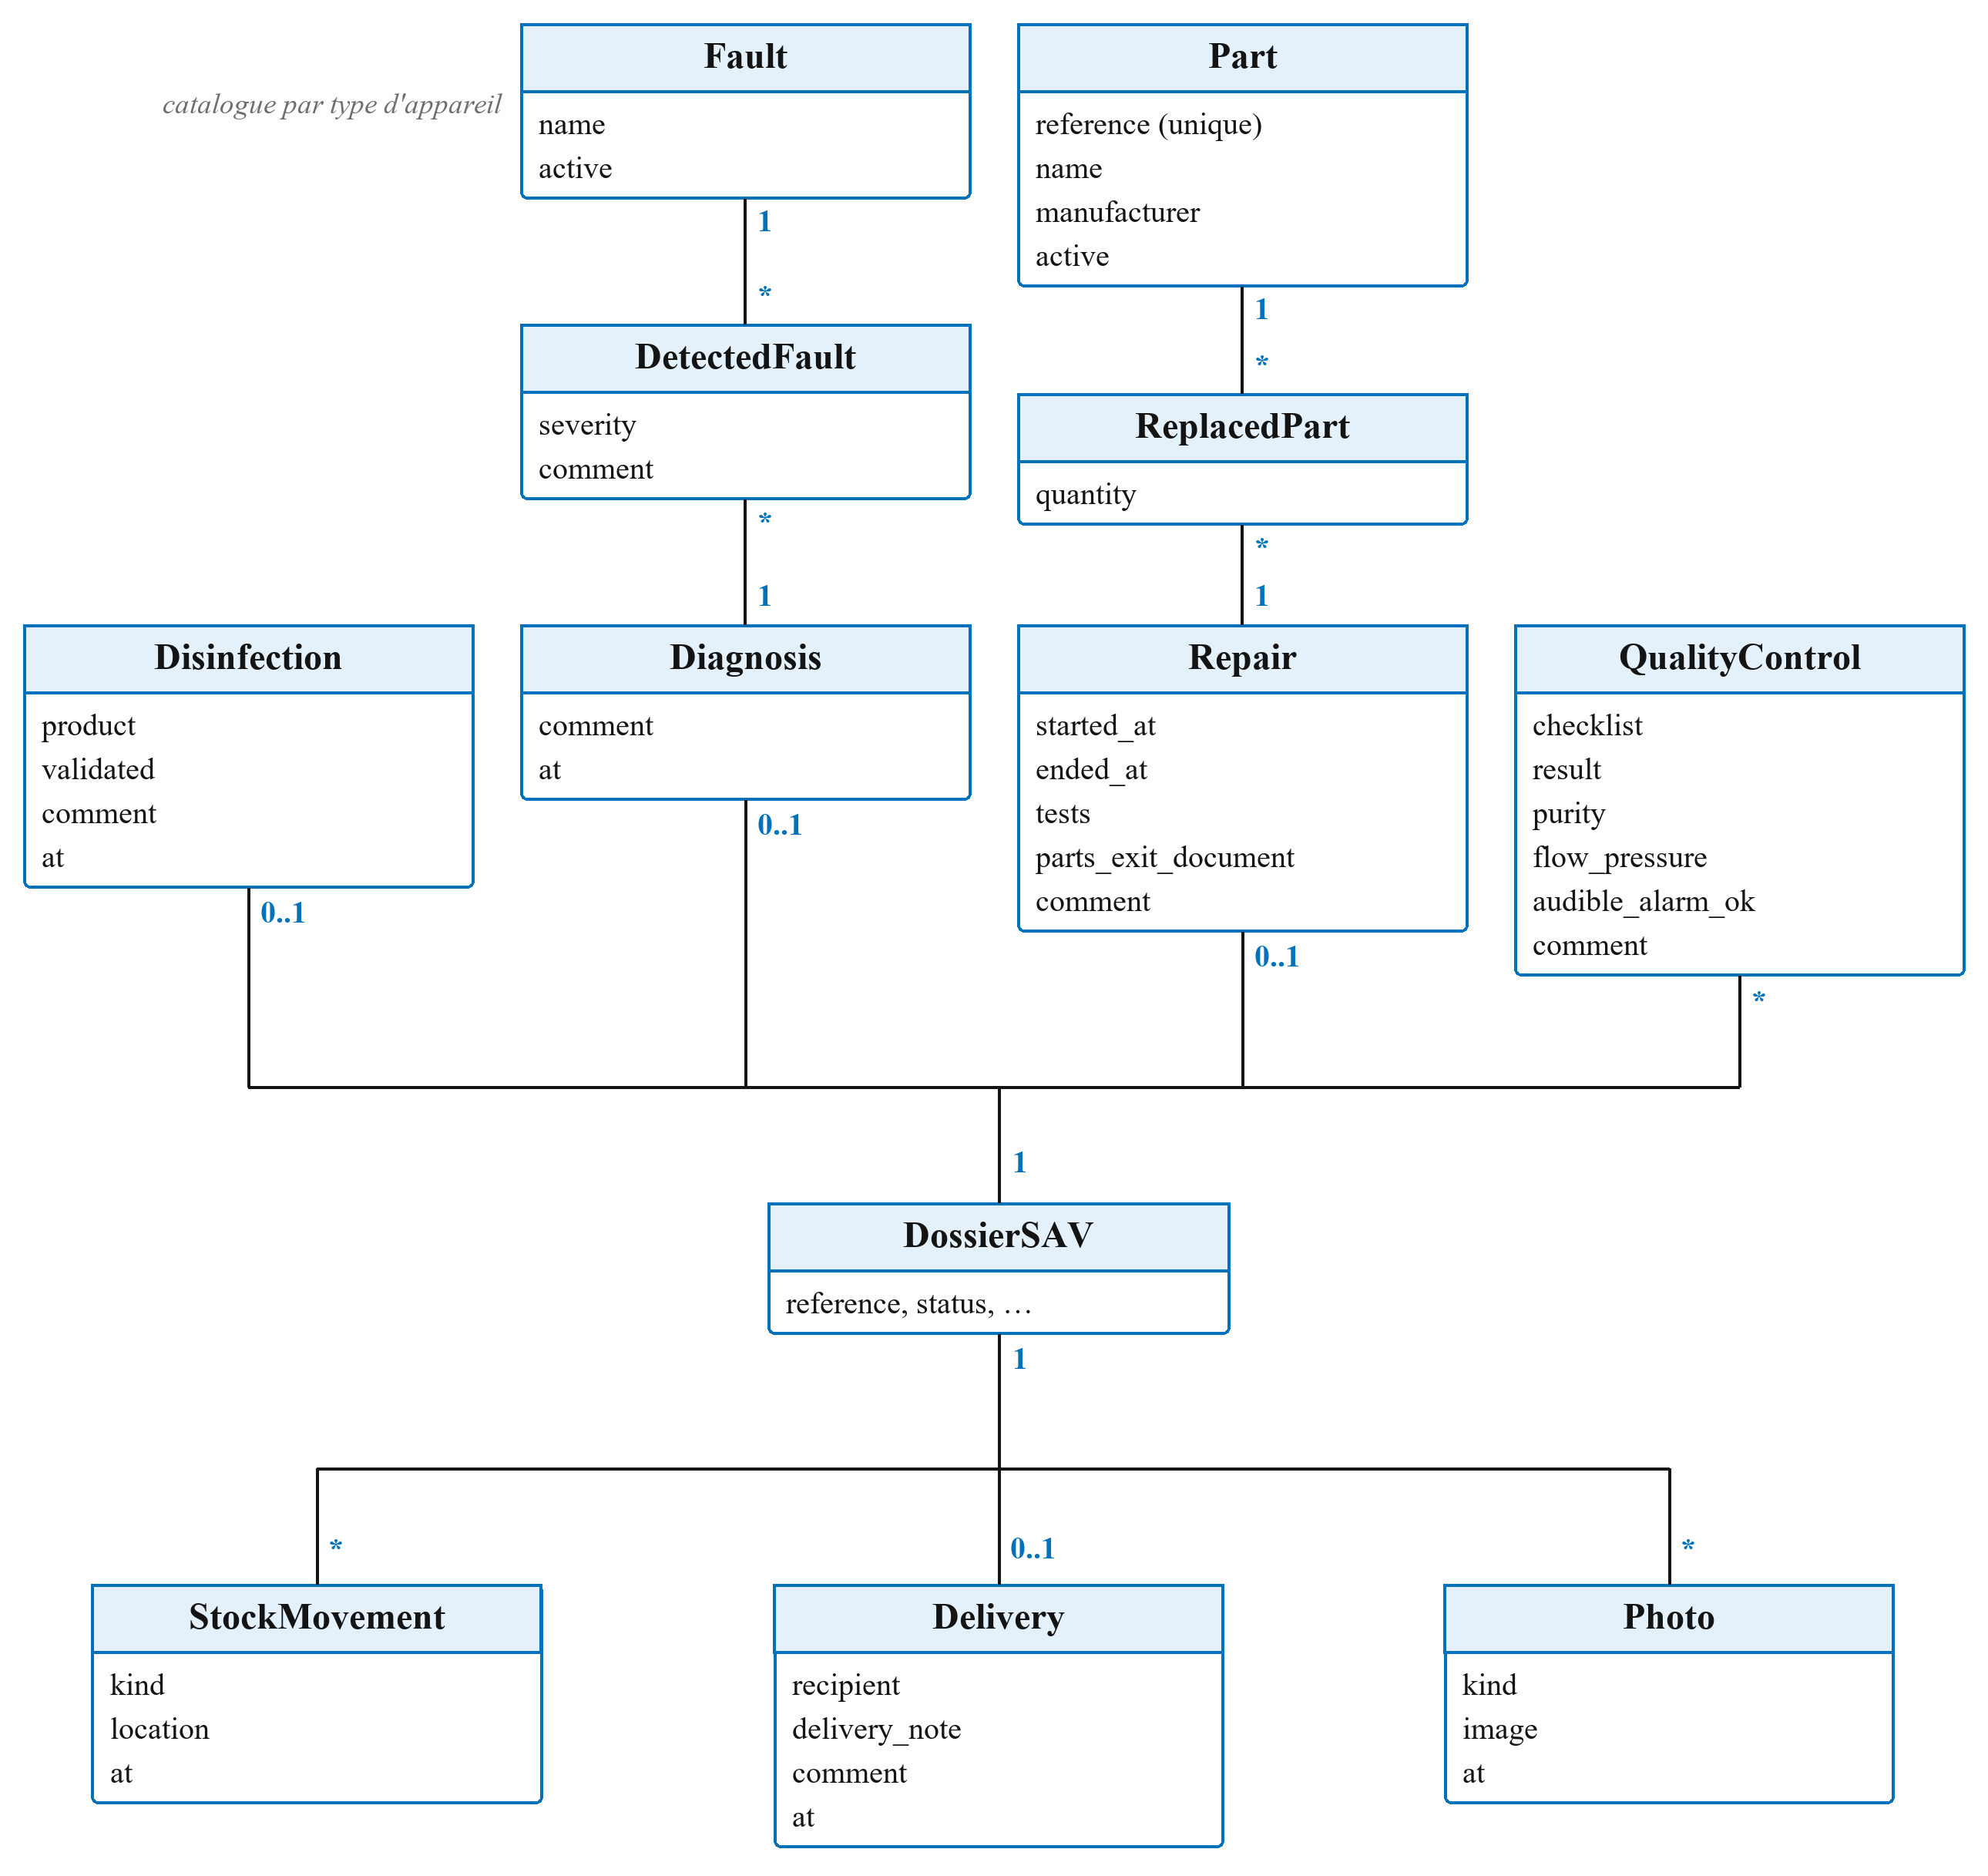
\includegraphics[width=15.5cm,height=18.5cm,keepaspectratio]{uml_classes_etapes.png}
\caption{Diagramme de classes : étapes rattachées au dossier SAV}
\end{figure}

Le modèle comprend 19 entités et 2 énumérations (annexe B), organisées autour de quatre groupes : utilisateurs, référentiel d'appareils (types, marques, modèles, appareils), dossier SAV et ses étapes, catalogues (pannes, pièces).

\subsection{Architecture}

L'application suit une architecture client / serveur en couches, fondée sur une API REST. Le frontend ne contient aucune règle métier : il appelle l'API, qui applique les règles dans une couche de services.

\begin{figure}[p]
\centering
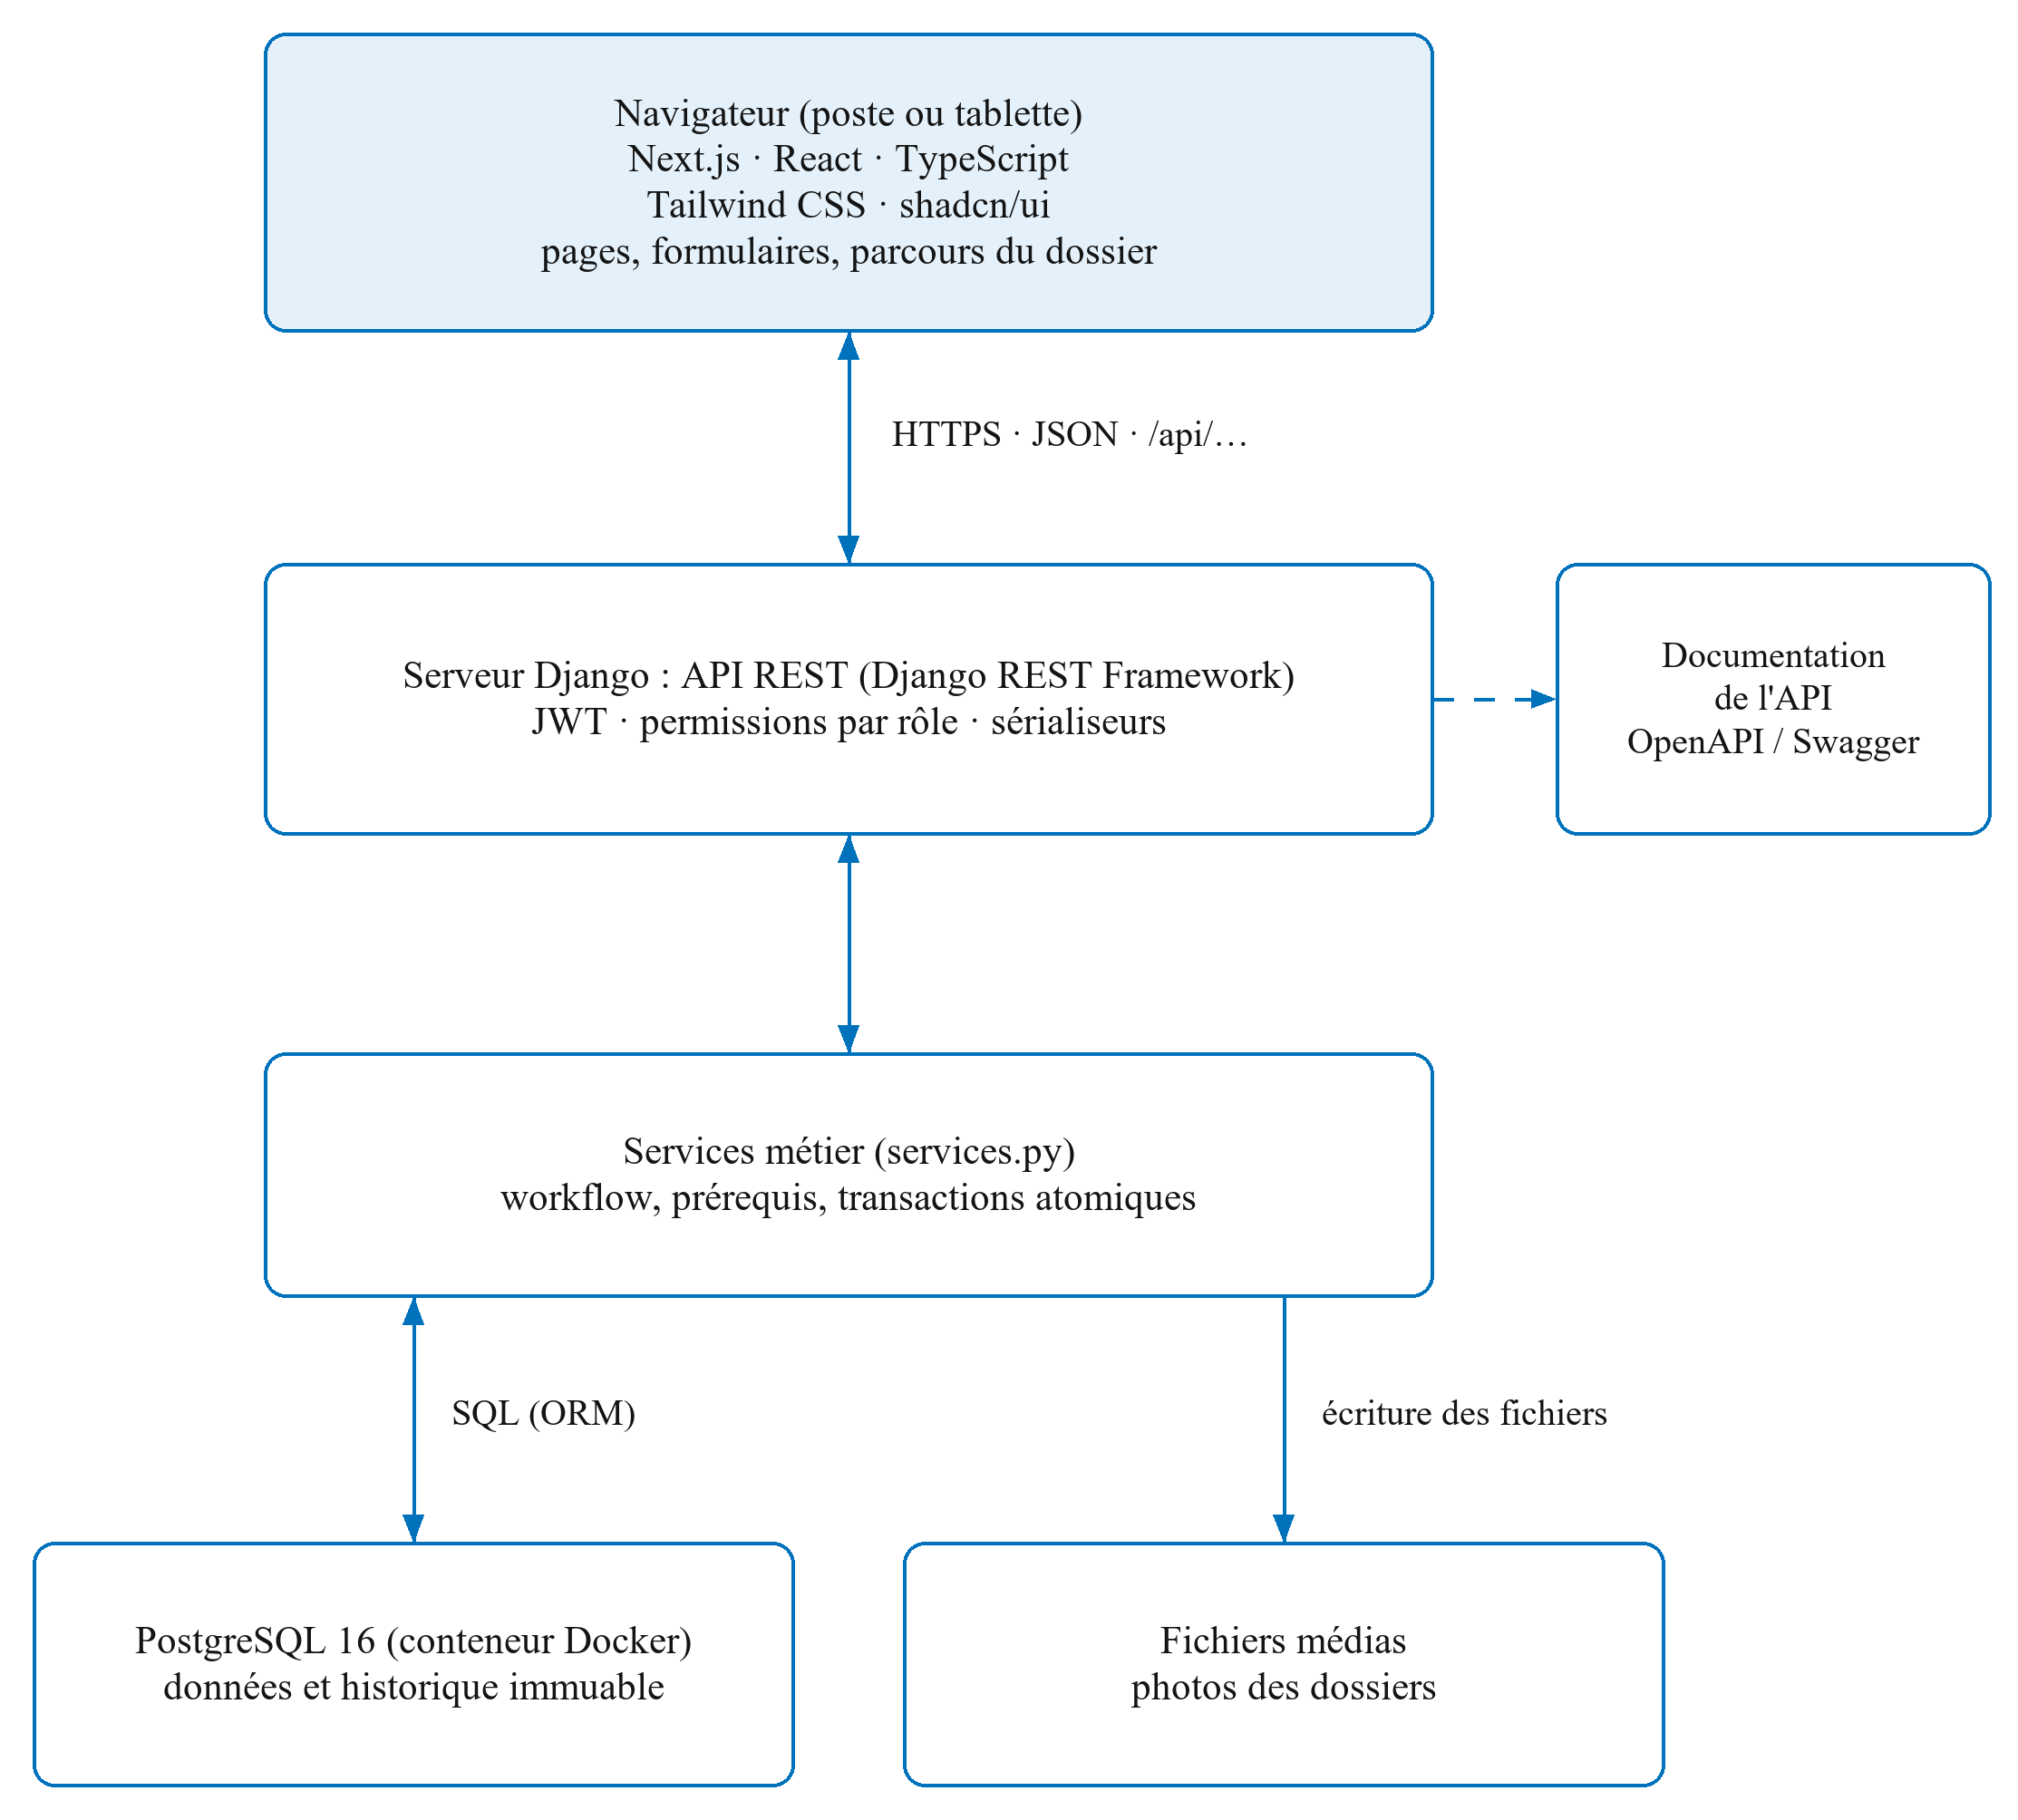
\includegraphics[width=15.5cm,height=18.5cm,keepaspectratio]{uml_architecture.png}
\caption{Architecture d'AirLiquide GMAO+}
\end{figure}

La conception initiale prévoyait une architecture modulaire orientée domaine, avec un module \texttt{maintenance} regroupant tout le cycle de vie, plus des modules \texttt{accounts}, \texttt{inventory}, \texttt{reports}, \texttt{dashboard} et \texttt{common}. Ce choix a été retenu. Le tableau suivant compare la cible initiale à ce qui a été réalisé.

\Needspace{14\baselineskip}

{\small\setstretch{1.05}\renewcommand{\arraystretch}{1.3}\arrayrulecolor{ALtexte}
\begin{longtable}{|>{\raggedright\arraybackslash}p{7.30cm}|>{\raggedright\arraybackslash}p{7.30cm}|}
\caption{Architecture cible et architecture réalisée}\\
\hline
\rowcolor{ALbleu} \sffamily\bfseries\color{white} Élément de l'architecture cible & \sffamily\bfseries\color{white} État dans l'application réalisée \\ \hline
\endfirsthead
\caption[]{Architecture cible et architecture réalisée (suite)}\\
\hline
\rowcolor{ALbleu} \sffamily\bfseries\color{white} Élément de l'architecture cible & \sffamily\bfseries\color{white} État dans l'application réalisée \\ \hline
\endhead
Modules \texttt{accounts}, \texttt{maintenance}, \texttt{inventory}, \texttt{dashboard}, \texttt{reports} & Réalisés ; \texttt{common} créé mais non utilisé \\ \hline
\rowcolor{ALgris} Services (règles métier hors des vues) & Réalisés : \texttt{maintenance/\allowbreak{}services.\allowbreak{}py} \\ \hline
Selectors et repositories & Non réalisés : jugés inutiles à cette taille de projet \\ \hline
\rowcolor{ALgris} Frontend web Next.js / TypeScript / Tailwind / shadcn/ui & Réalisé \\ \hline
Application mobile Flutter & Non réalisée (prévue comme extension) \\ \hline
\rowcolor{ALgris} Docker & Partiel : seule la base PostgreSQL est conteneurisée \\ \hline
Rapports PDF, notifications, QR code & Non réalisés (perspectives) \\ \hline
\end{longtable}
}

\subsection{Sécurité}

\begin{itemize}
  \item \textbf{Authentification JWT} : le jeton d'accès reste en mémoire dans le navigateur ; le jeton de rafraîchissement est placé dans un cookie \texttt{HttpOnly}, inaccessible au code JavaScript (protection contre le vol de jeton) ;
  \item \textbf{limitation du nombre de tentatives} de connexion (10 par minute) ;
  \item \textbf{permissions par rôle} appliquées côté serveur, quelles que soient les actions de l'interface ;
  \item \textbf{validation côté serveur} de toutes les entrées ; contrôle des photos (formats JPEG, PNG, WebP, taille maximale 5 Mo, vérification du contenu) ;
  \item \textbf{exports CSV} protégés contre l'injection de formules dans les tableurs ;
  \item \textbf{secrets} (clé, mots de passe de base) hors du dépôt, dans un fichier d'environnement non versionné.
\end{itemize}

Le diagramme de séquence suivant détaille le cycle d'authentification : connexion, conservation du jeton d'accès en mémoire et renouvellement grâce au cookie.

\begin{figure}[p]
\centering
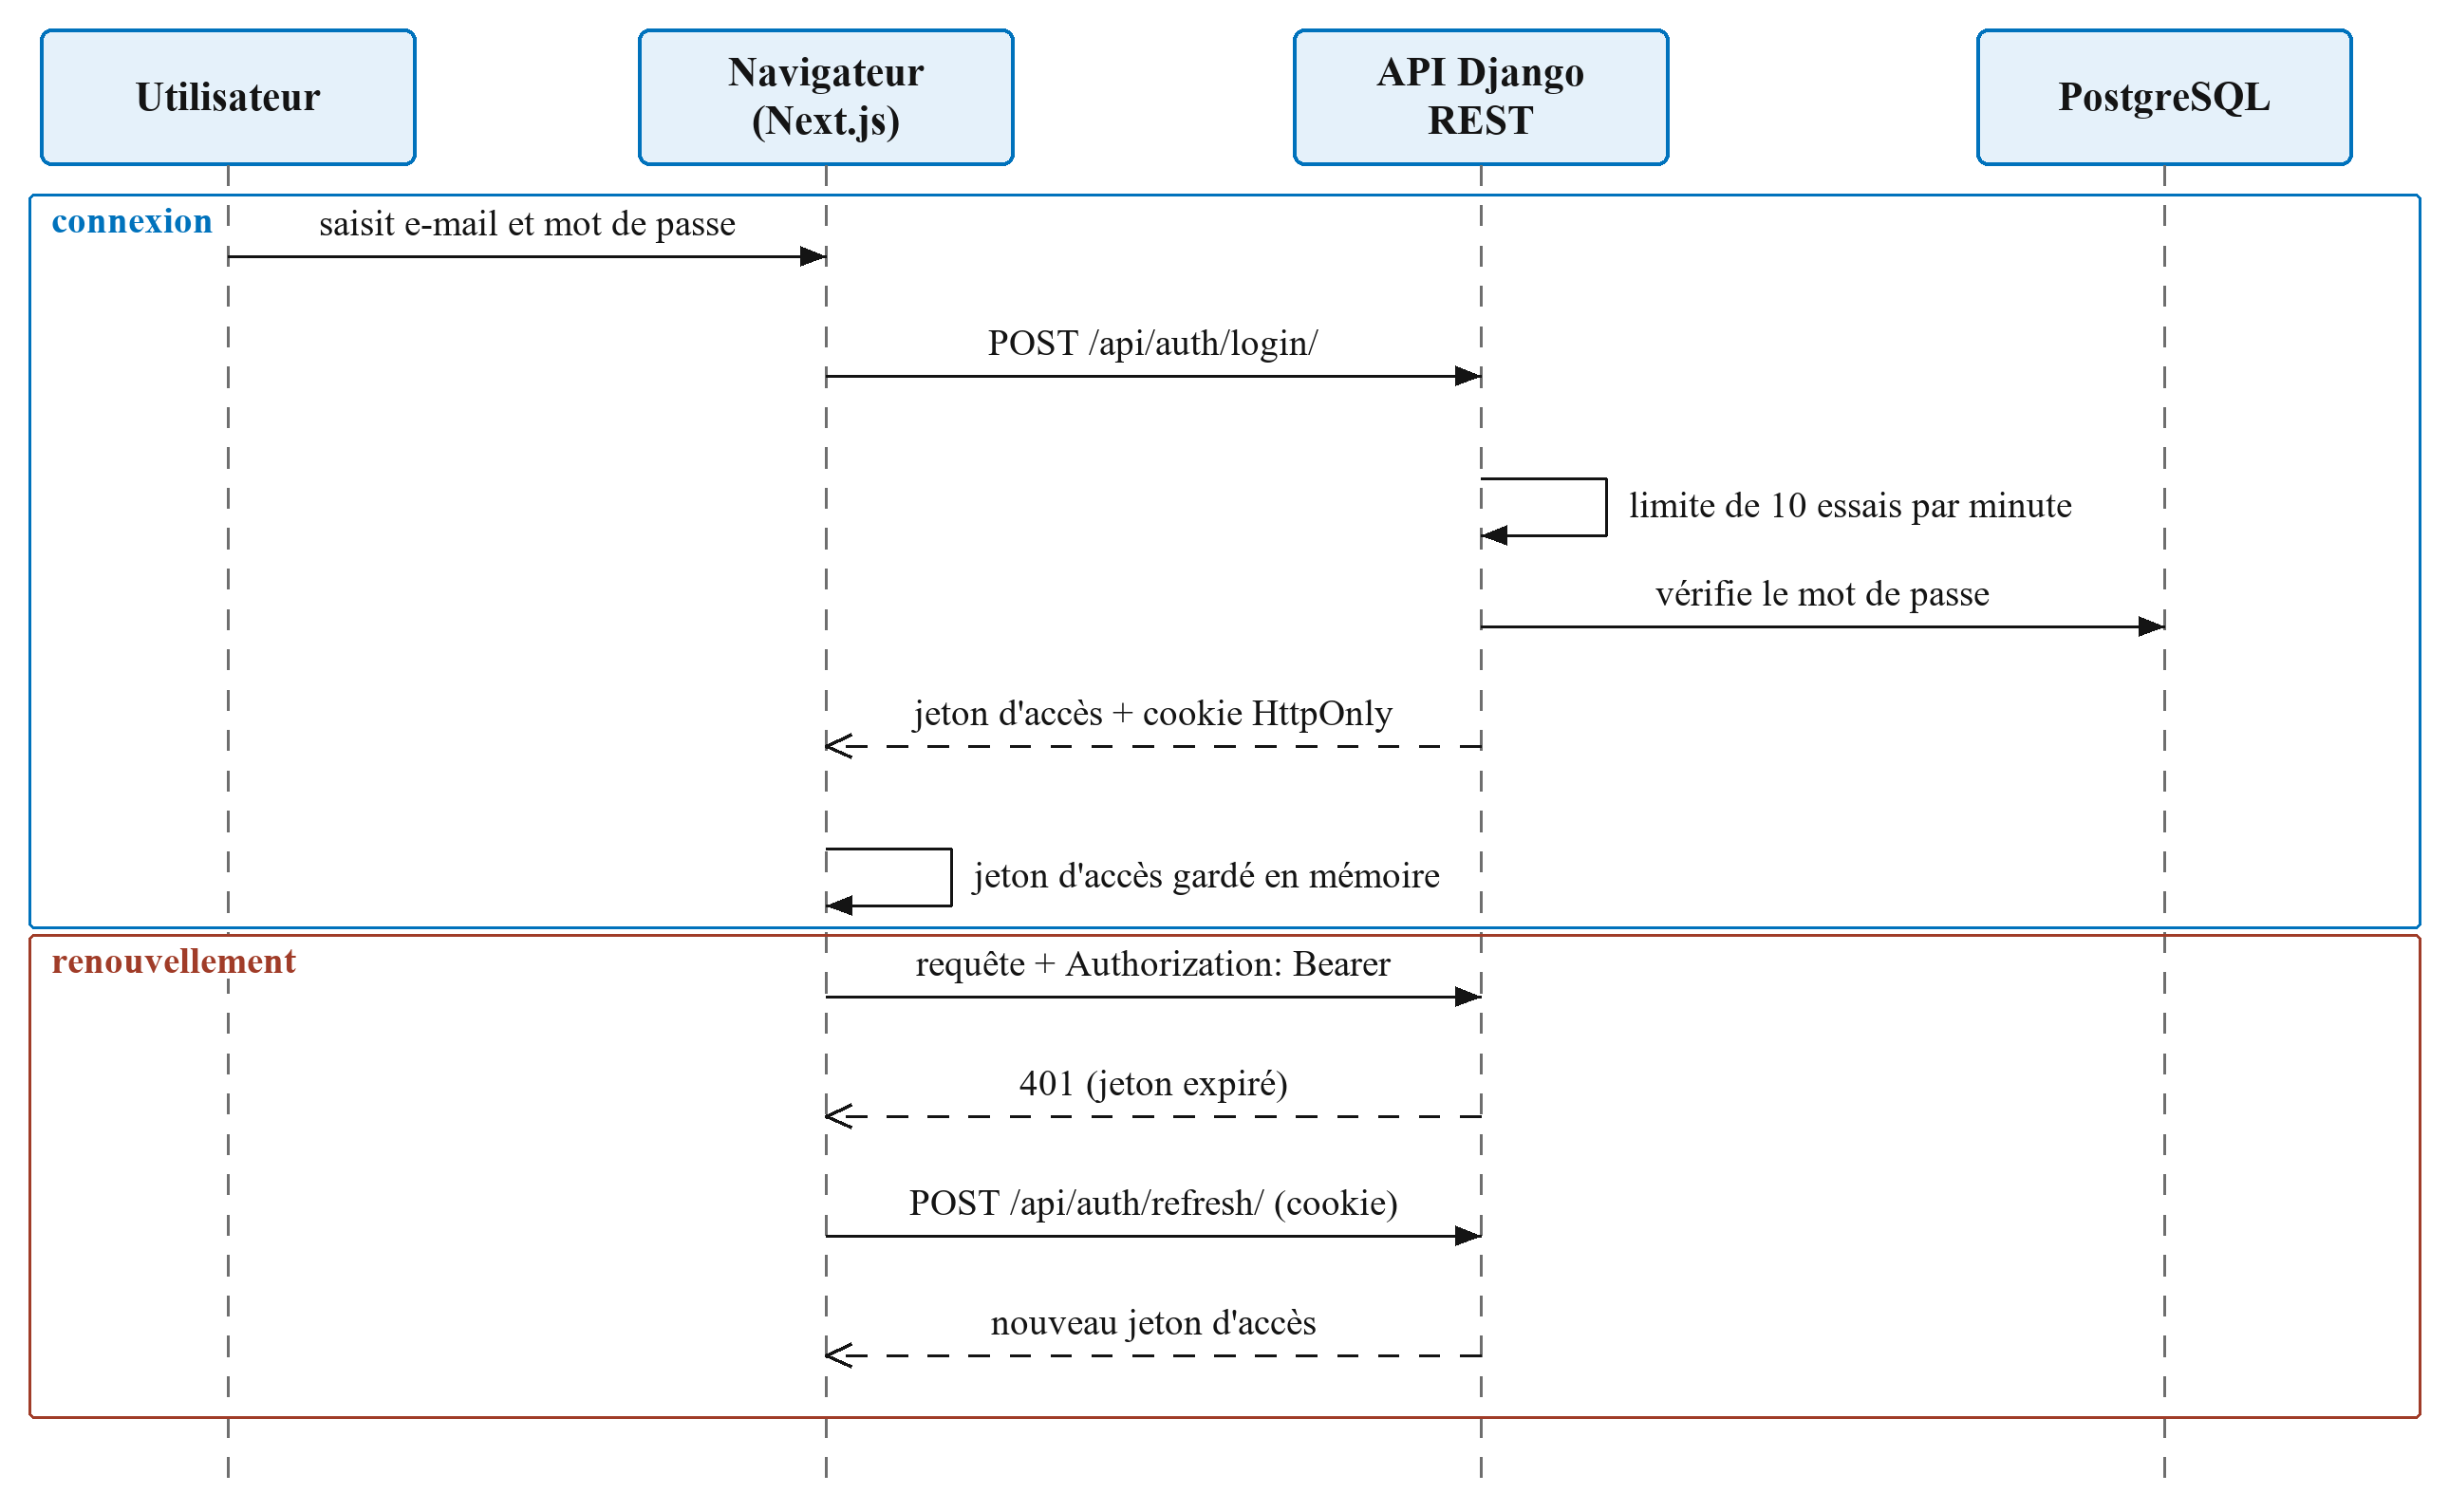
\includegraphics[width=15.5cm,height=18.5cm,keepaspectratio]{uml_sequence_auth.png}
\caption{Diagramme de séquence : authentification et renouvellement du jeton}
\end{figure}

\section{Réalisation}

\Needspace{15\baselineskip}
\subsection{Environnement technique}

{\small\setstretch{1.05}\renewcommand{\arraystretch}{1.3}\arrayrulecolor{ALtexte}
\begin{longtable}{|>{\raggedright\arraybackslash}p{3.20cm}|>{\raggedright\arraybackslash}p{11.41cm}|}
\caption{Environnement technique (versions relevées dans les fichiers de dépendances)}\\
\hline
\rowcolor{ALbleu} \sffamily\bfseries\color{white} Couche & \sffamily\bfseries\color{white} Technologies et versions \\ \hline
\endfirsthead
\caption[]{Environnement technique (versions relevées dans les fichiers de dépendances) (suite)}\\
\hline
\rowcolor{ALbleu} \sffamily\bfseries\color{white} Couche & \sffamily\bfseries\color{white} Technologies et versions \\ \hline
\endhead
Backend & Python 3.10, Django 5.2.16, Django REST Framework 3.17.1, SimpleJWT 5.5.1, drf-spectacular 0.30.0, django-cors-headers 4.9.0, Pillow 12.3.0 \\ \hline
\rowcolor{ALgris} Base de données & PostgreSQL 16 (conteneur Docker) ; SQLite en repli pour le développement \\ \hline
Frontend & Next.js 16.4.3, React 19.3.0, TypeScript 5, Tailwind CSS 4, shadcn/ui, lucide-react, sonner \\ \hline
\rowcolor{ALgris} Documentation API & OpenAPI / Swagger généré automatiquement (\texttt{/\allowbreak{}api/\allowbreak{}docs/\allowbreak{}}) \\ \hline
Outils & Git et GitHub, Docker Compose, Chrome et outils de développement \\ \hline
\end{longtable}
}

\subsection{Le backend}

Le backend est organisé en applications Django. Les \textbf{vues} reçoivent la requête et délèguent ; les \textbf{sérialiseurs} valident les entrées ; les \textbf{services} (\texttt{maintenance/\allowbreak{}services.\allowbreak{}py}) exécutent les règles métier dans des transactions atomiques : réception, désinfection, diagnostic, réparation, contrôle qualité, entrée en stock, livraison et changement de statut. Chaque service verrouille le dossier, vérifie le statut attendu, enregistre l'étape, fait avancer le statut et écrit l'historique en une seule opération.

L'API expose des points d'accès REST documentés (annexe A). Les actions de workflow sont de simples \texttt{POST} sur le dossier (par exemple \texttt{/\allowbreak{}api/\allowbreak{}dossiers/\allowbreak{}\{id\}/\allowbreak{}quality-\allowbreak{}control/\allowbreak{}}), ce qui rend l'enregistrement d'une étape et le changement de statut indissociables.

\begin{figure}[p]
\centering
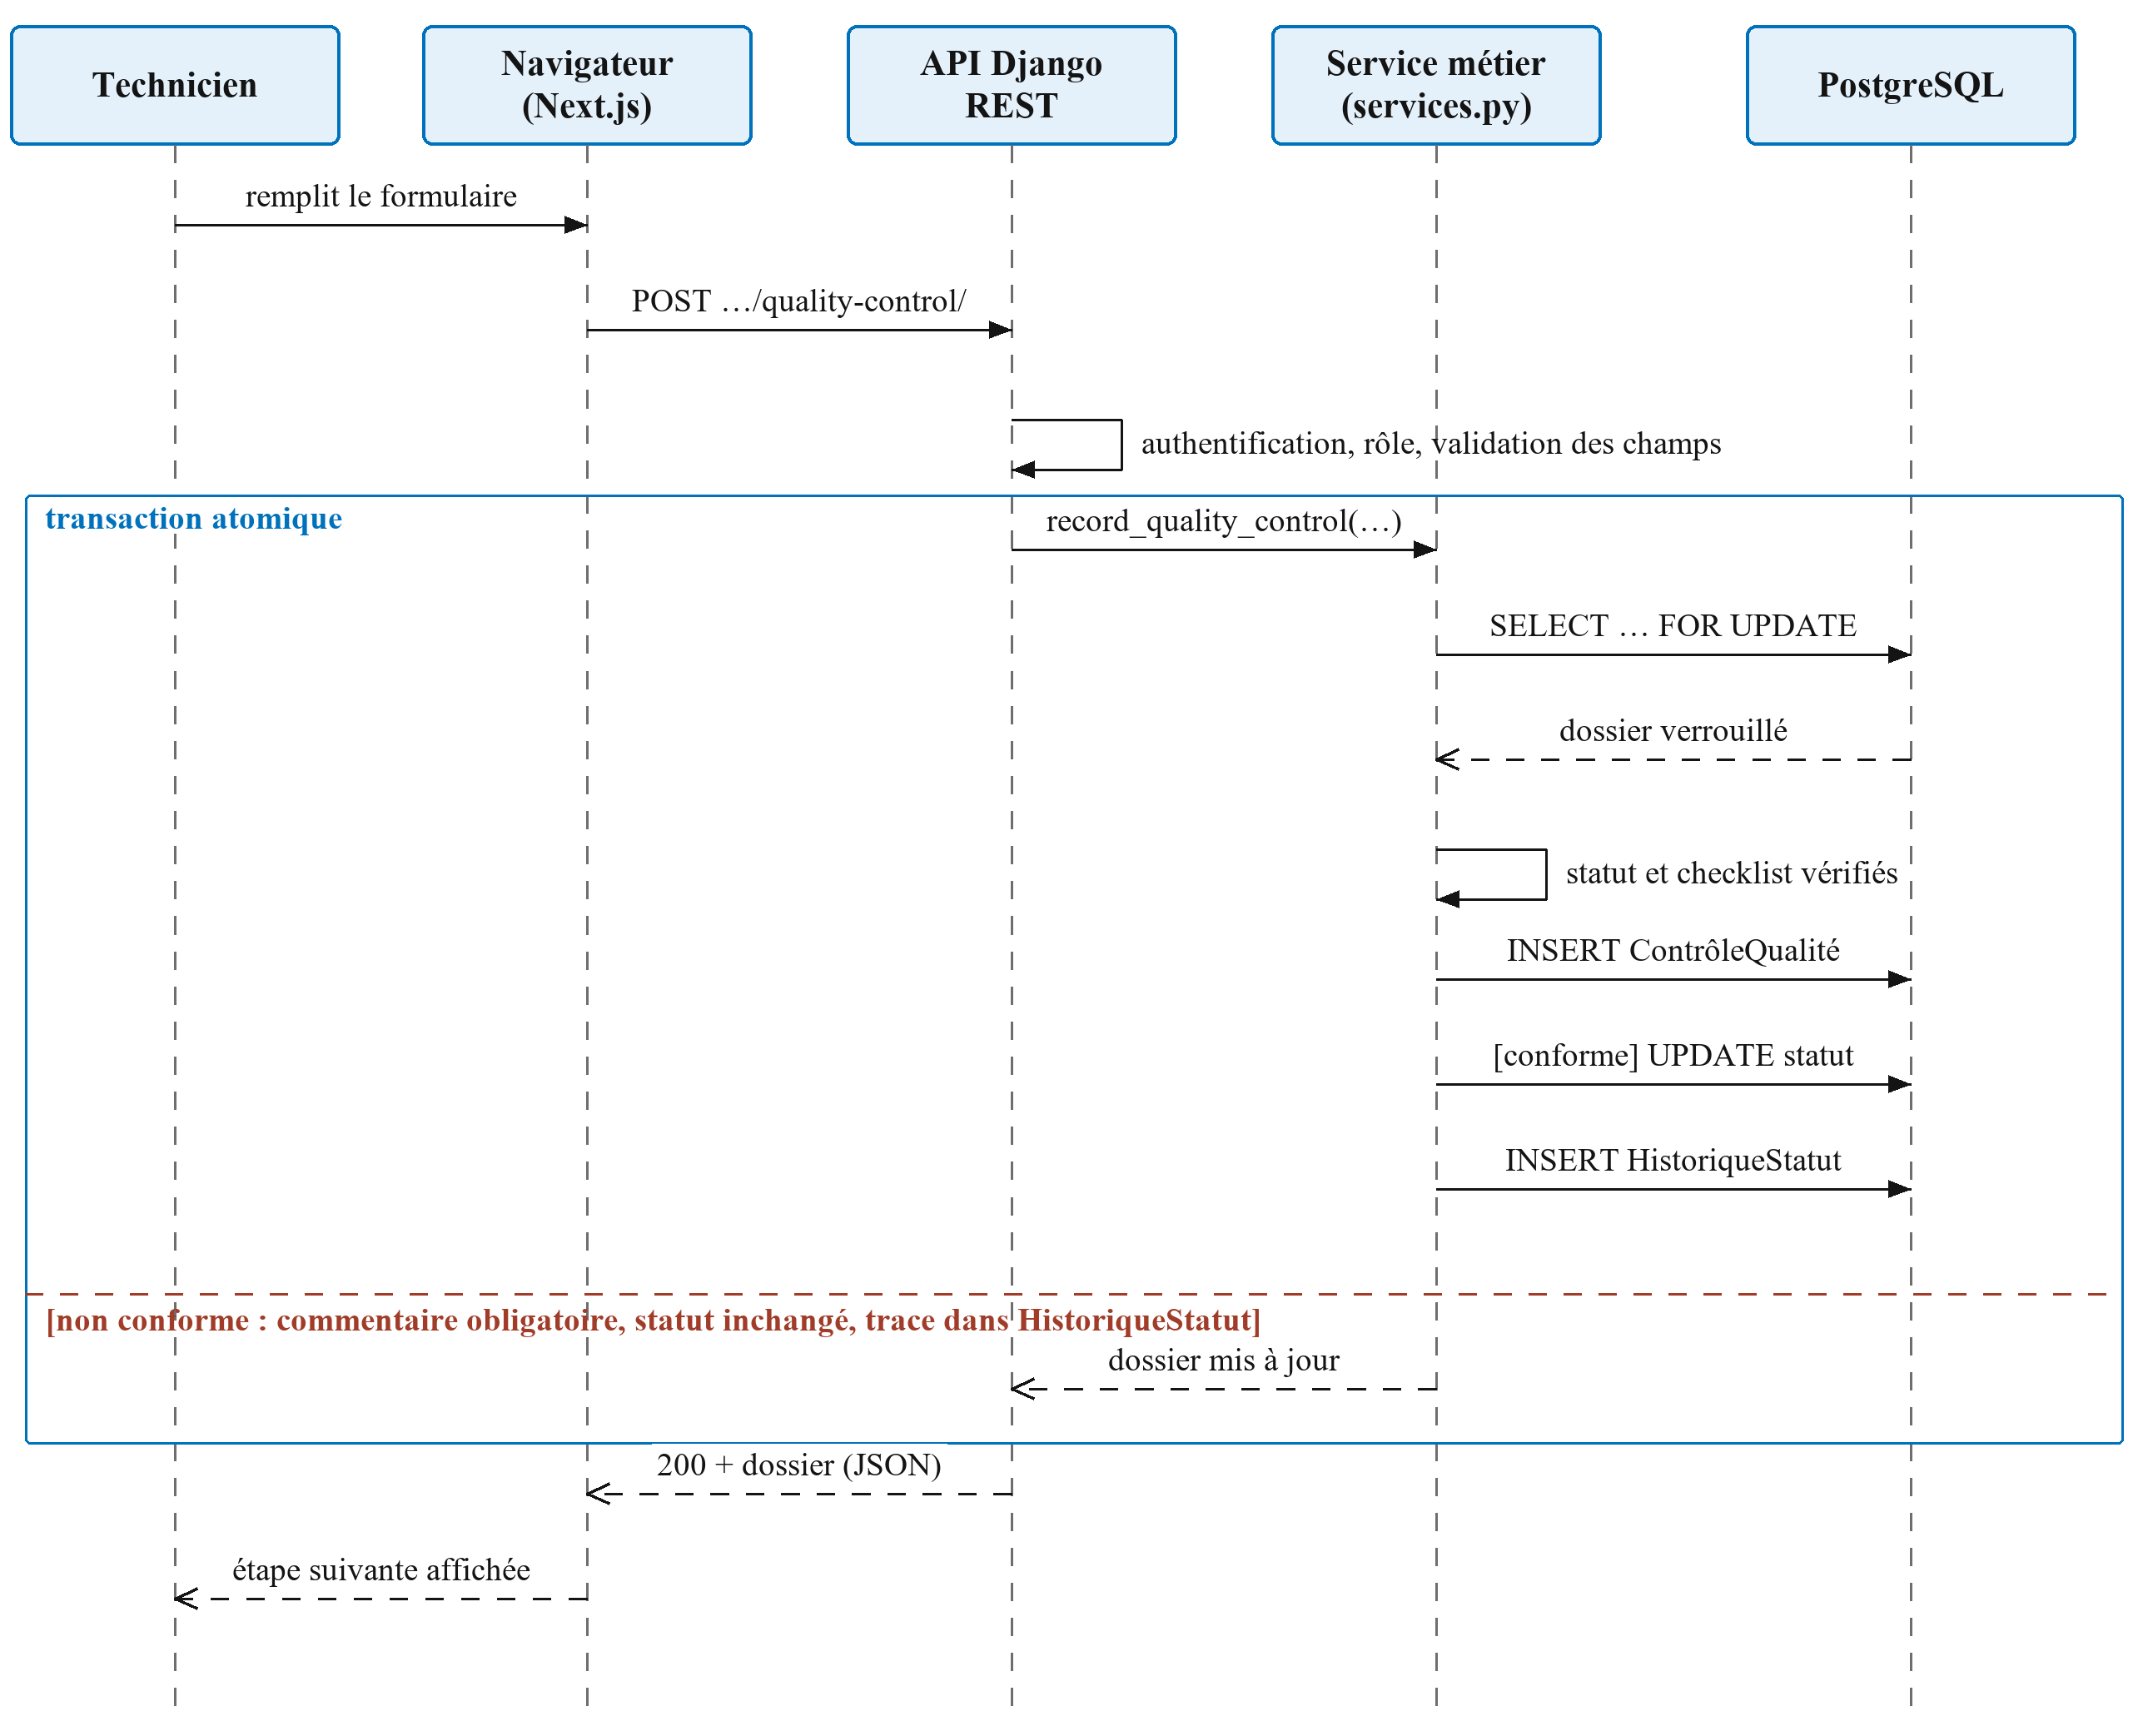
\includegraphics[width=15.5cm,height=18.5cm,keepaspectratio]{uml_sequence_etape.png}
\caption{Diagramme de séquence : enregistrement d'une étape (contrôle qualité)}
\end{figure}

\subsection{Le questionnaire de retour}

Le questionnaire en ligne existant a été intégré à l'application sous la forme d'une \textbf{annonce de retour} : avant l'arrivée de l'appareil, un utilisateur saisit le numéro de série, l'état visuel, les accessoires manquants, l'identifiant de retour et le statut biologique. À l'arrivée, le technicien choisit le retour annoncé dans l'écran de réception : les réponses sont reprises, le numéro de série est verrouillé et l'annonce est rattachée au dossier. Une annonce ne peut être réceptionnée qu'une seule fois.

\begin{figure}[!htb]
\centering
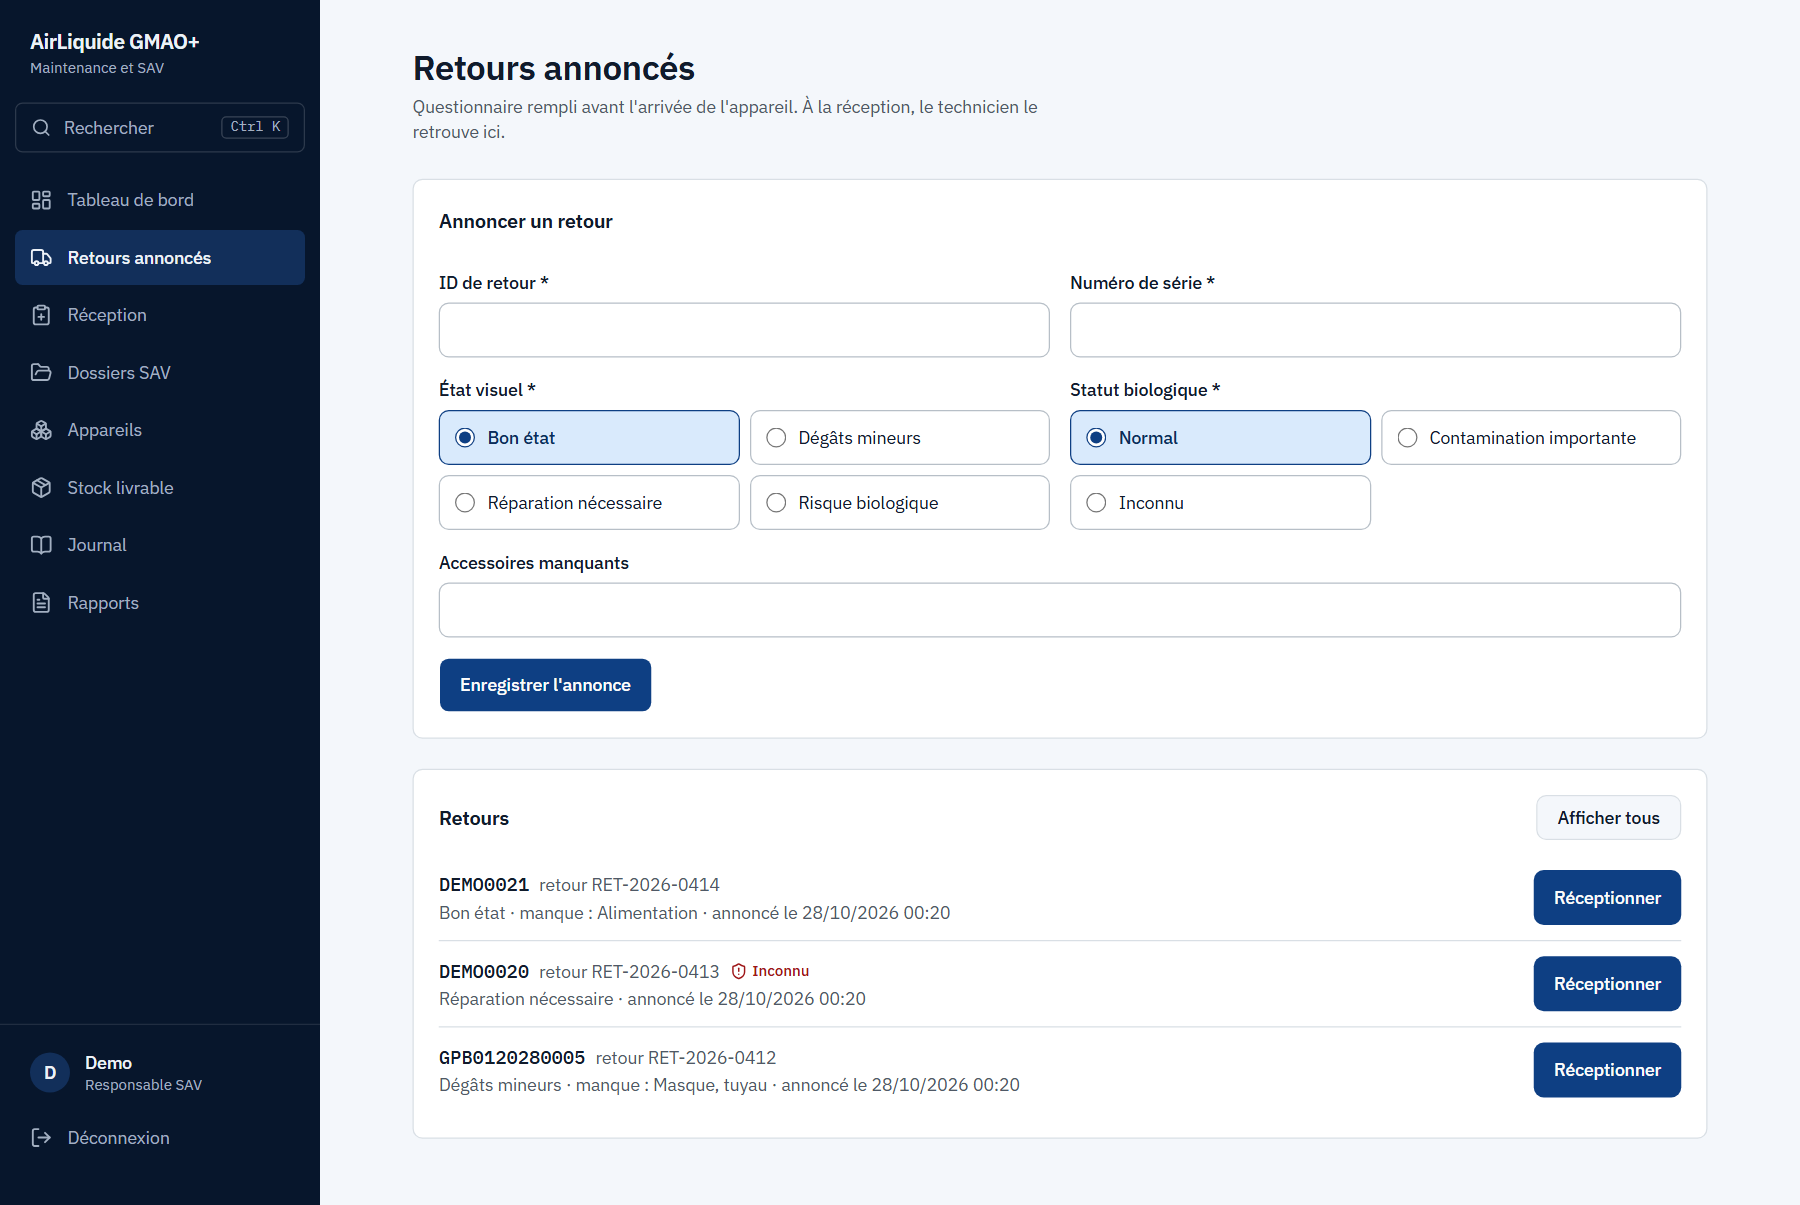
\includegraphics[width=15.0cm,height=17.5cm,keepaspectratio]{cap_retours.png}
\caption{Écran des retours annoncés (données de démonstration)}
\end{figure}

\begin{figure}[!htb]
\centering
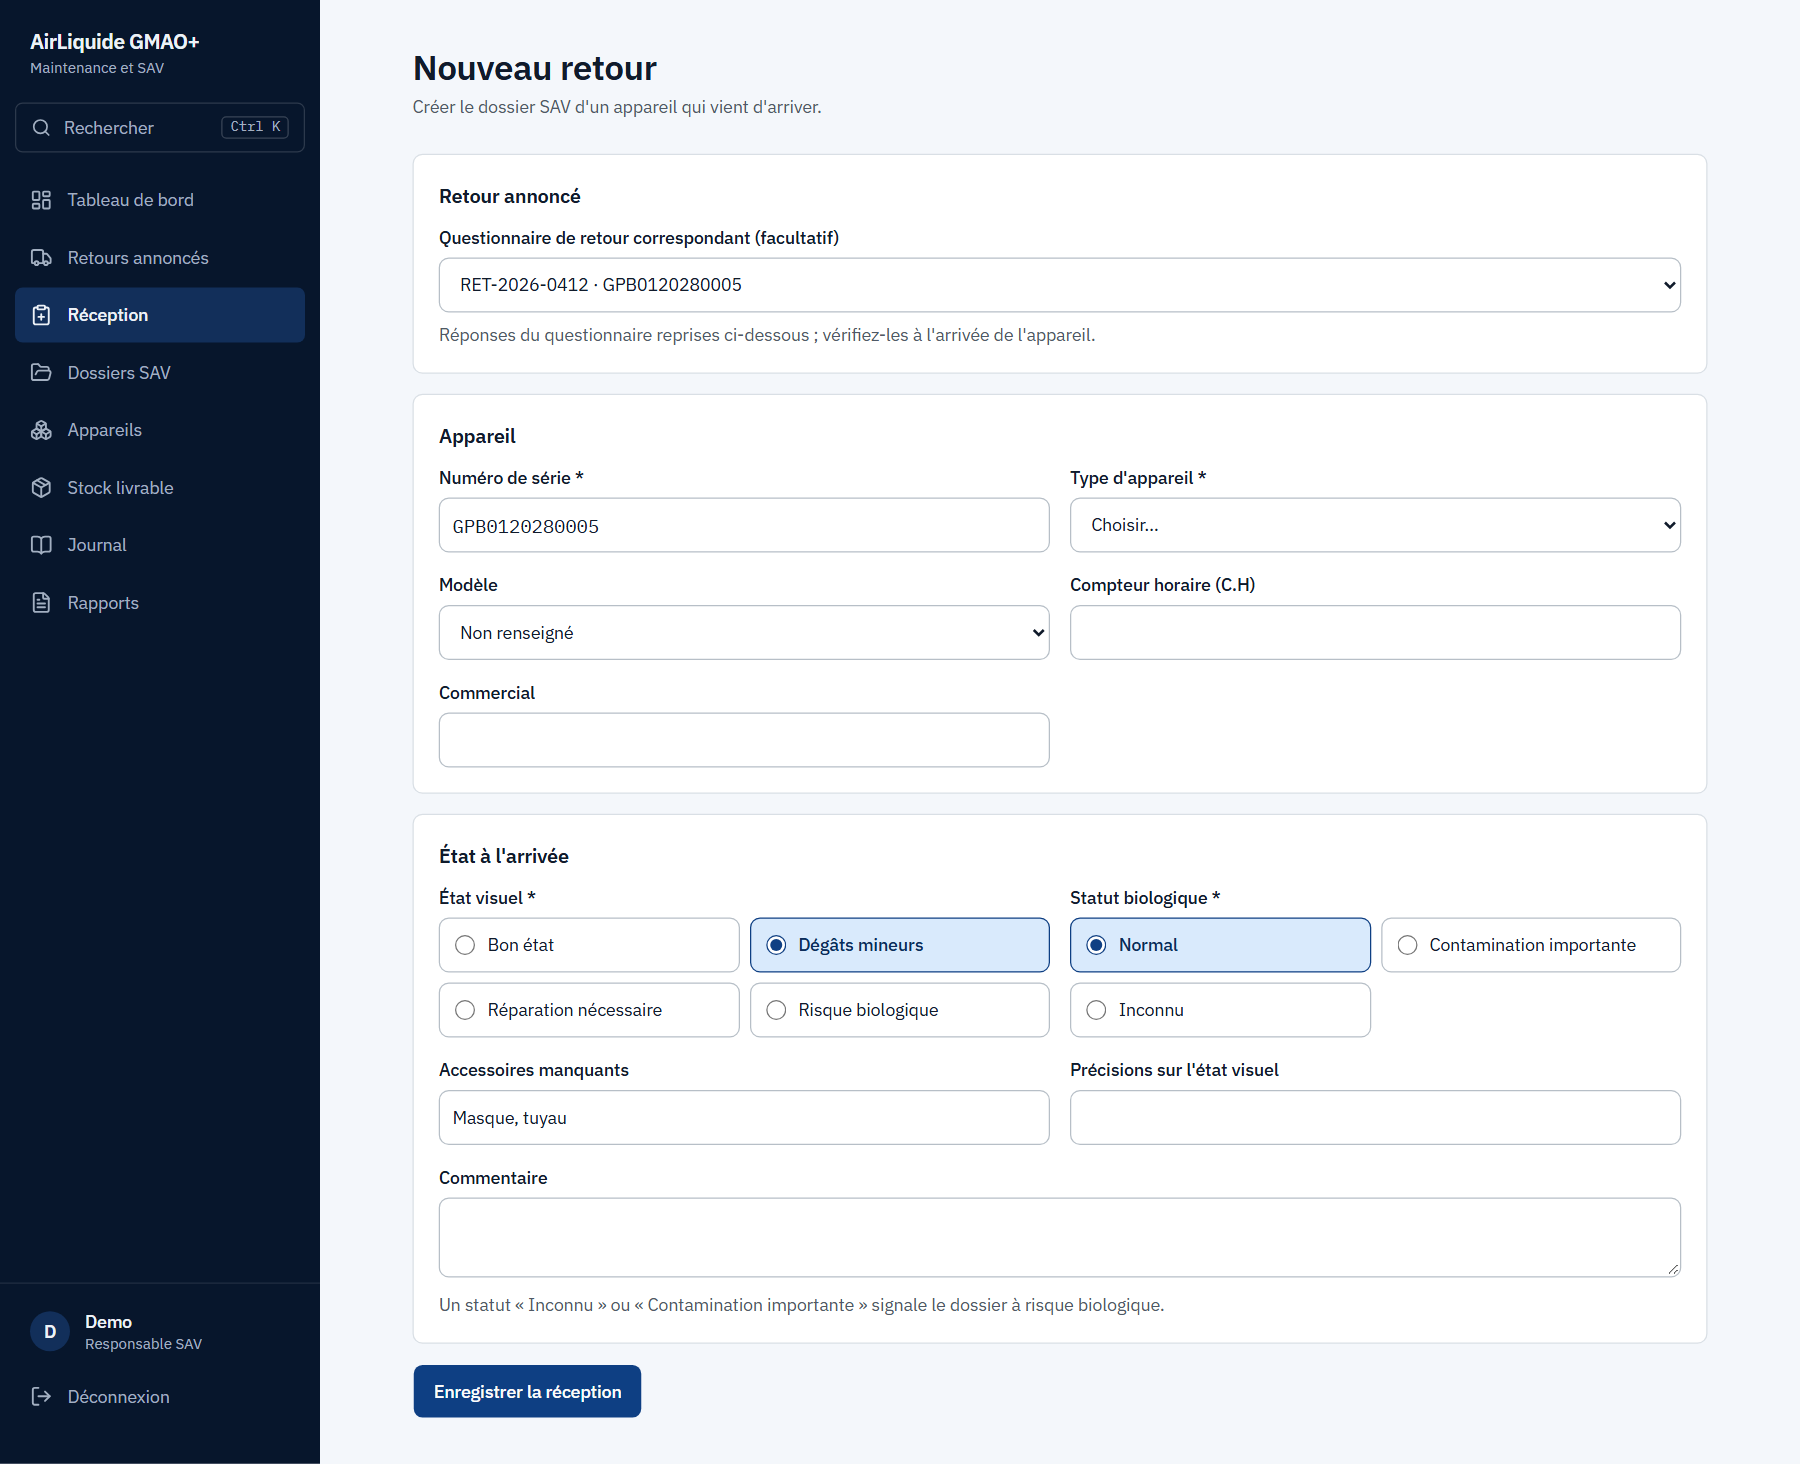
\includegraphics[width=14.0cm,height=17.5cm,keepaspectratio]{cap_reception.png}
\caption{Écran de réception d'un appareil (données de démonstration)}
\end{figure}

\subsection{Le journal de maintenance}

Le registre papier a été reproduit sous forme numérique. Le journal n'est \textbf{pas une table à saisir} : il est calculé à partir des dossiers, une ligne par retour, avec les douze colonnes du registre (annexe D). Il ne peut donc pas diverger des dossiers. L'écran propose des filtres (année, mois, type, numéro de série), l'impression et l'export CSV. Pour alimenter les colonnes du registre, le compteur horaire est saisi à la réception ; la pureté, le débit ou la pression et l'alarme sonore au contrôle qualité ; le document de sortie des pièces à la réparation.

\begin{figure}[!htb]
\centering
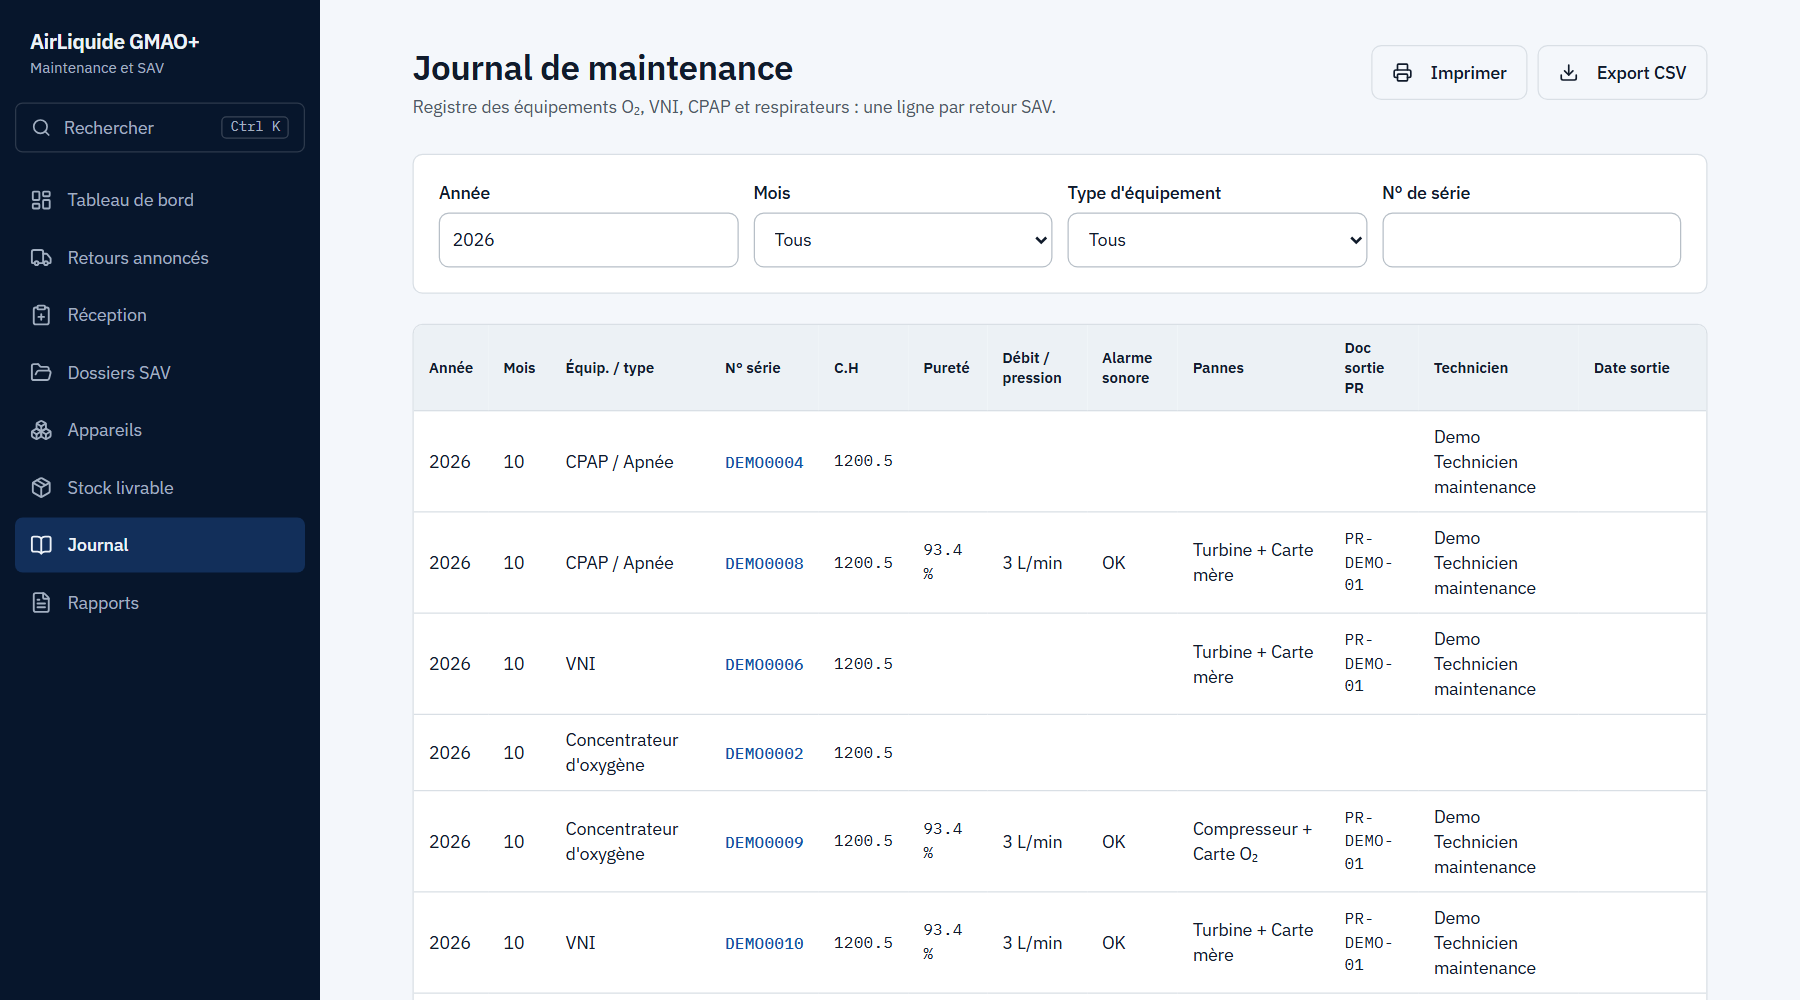
\includegraphics[width=15.0cm,height=17.5cm,keepaspectratio]{cap_journal.png}
\caption{Journal de maintenance numérique (données de démonstration)}
\end{figure}

\subsection{Le frontend et l'expérience utilisateur}

L'interface est en français et vise l'usage en atelier : cibles tactiles d'au moins 44 pixels, contrastes suffisants, statuts toujours accompagnés d'un libellé et d'une icône (jamais la couleur seule), navigation au clavier. Plusieurs choix répondent à des besoins observés :

\begin{itemize}
  \item le \textbf{tableau de bord} montre la charge de l'atelier par poste (à désinfecter, à diagnostiquer, etc.) et la liste des dossiers à traiter en premier, du plus ancien au plus récent ;
  \item le \textbf{dossier} est présenté comme un parcours vertical : les étapes terminées se résument sur place et le formulaire de l'étape en cours s'ouvre à sa position ;
  \item la \textbf{recherche rapide} (Ctrl + K) retrouve un appareil par son numéro de série ;
  \item des \textbf{confirmations} (notifications) signalent chaque enregistrement ; les erreurs sont expliquées en clair.
\end{itemize}

\begin{figure}[!htb]
\centering
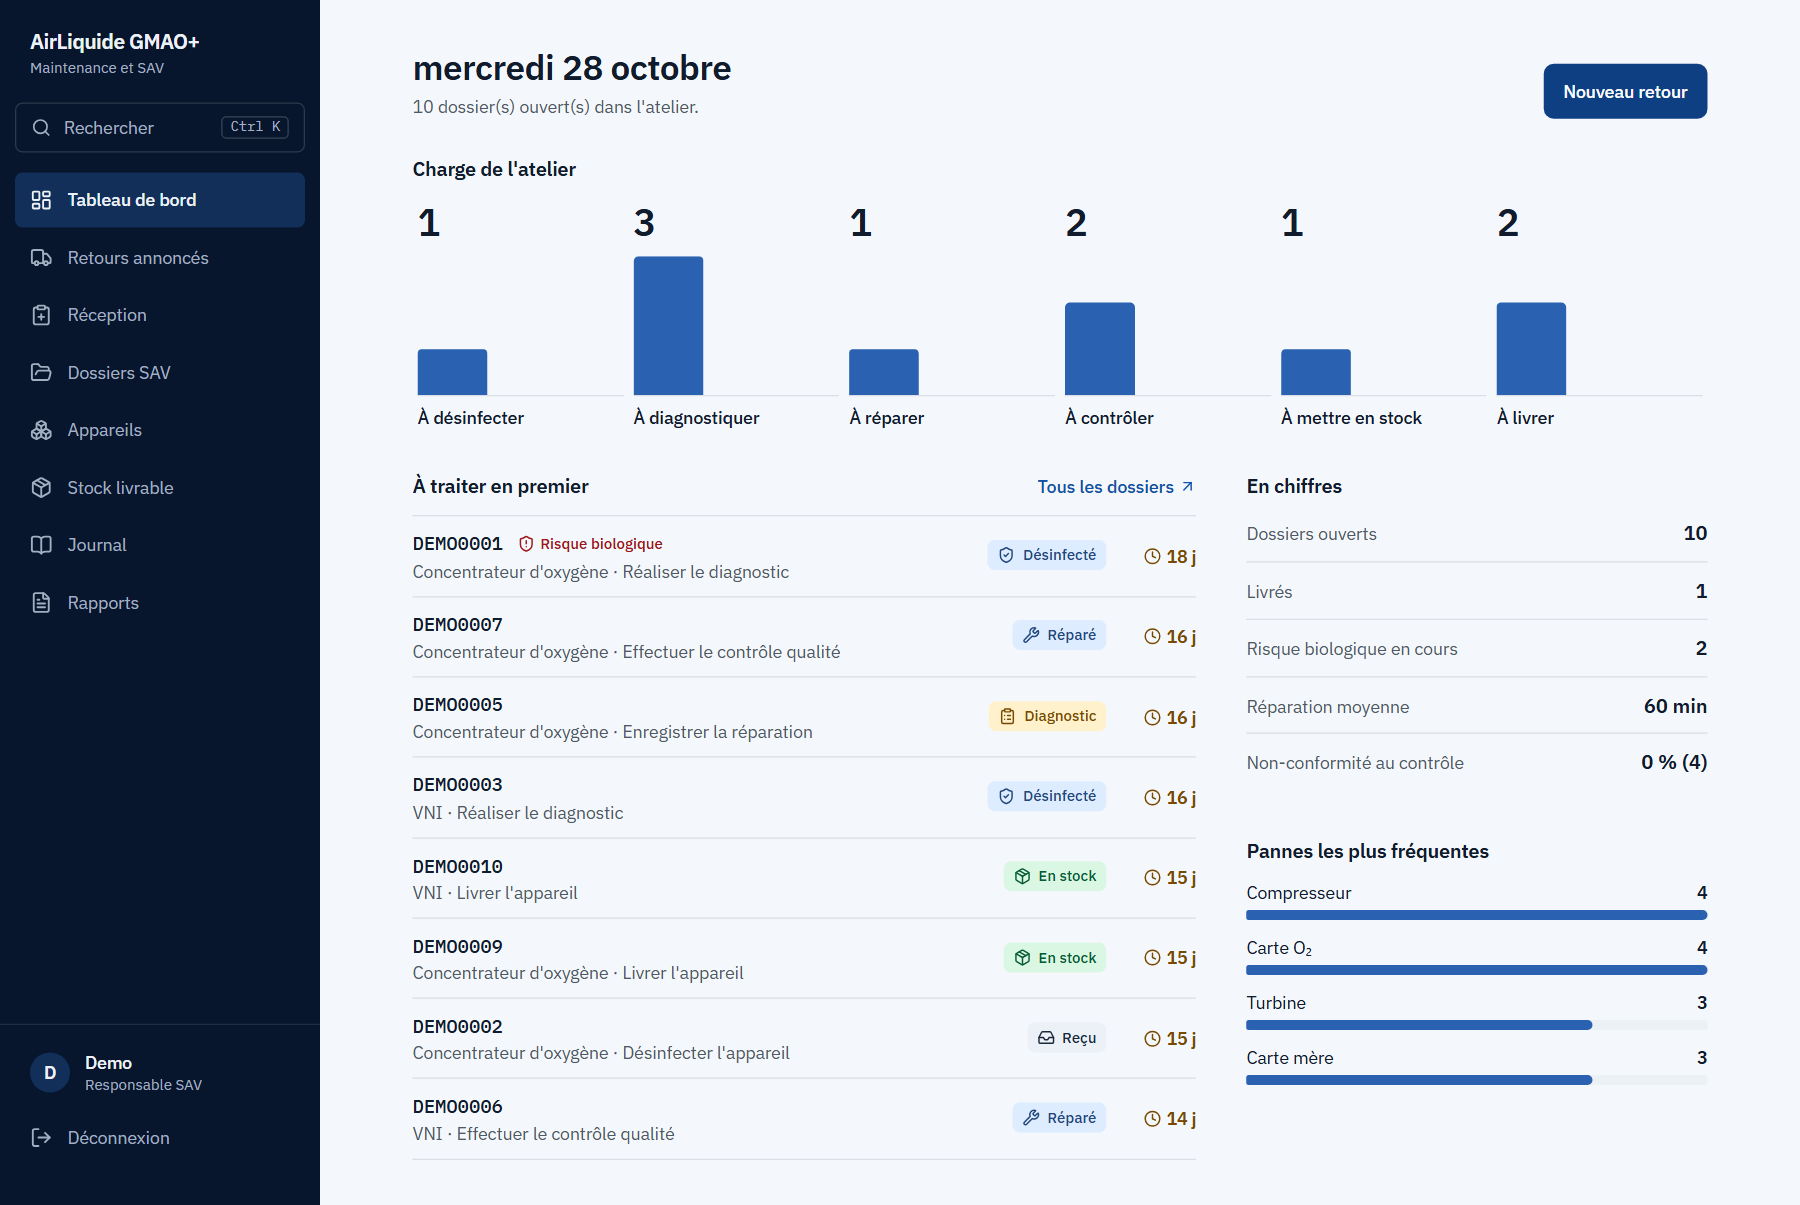
\includegraphics[width=15.5cm,height=17.5cm,keepaspectratio]{cap_tableau_de_bord.png}
\caption{Tableau de bord (données de démonstration)}
\end{figure}

\begin{figure}[!htb]
\centering
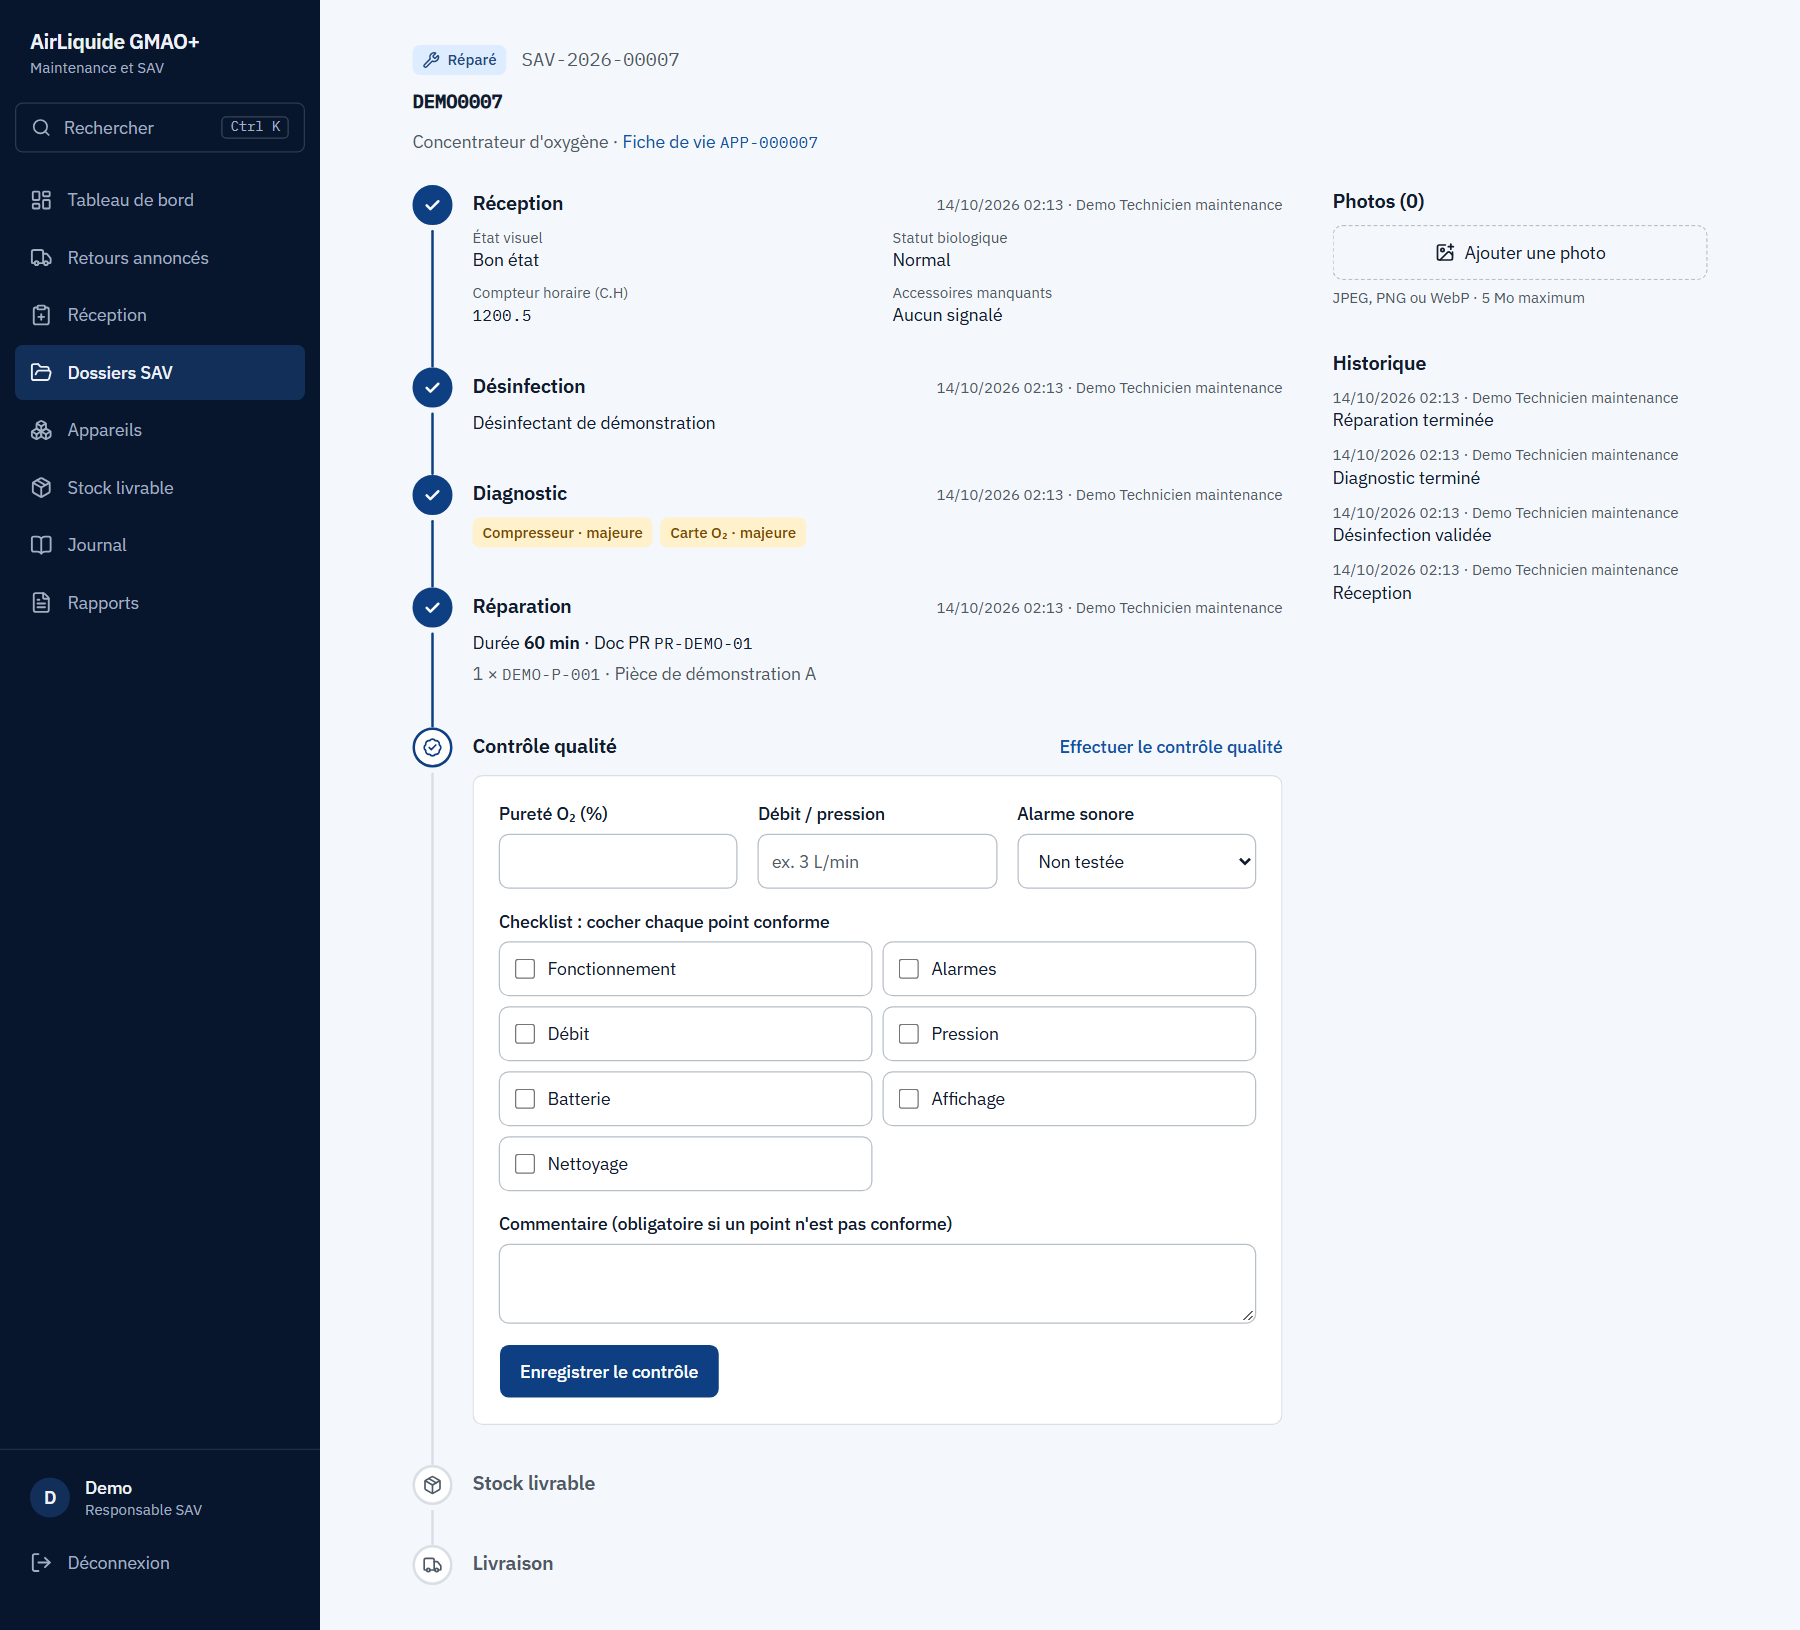
\includegraphics[width=15.0cm,height=17.5cm,keepaspectratio]{cap_dossier_qc.png}
\caption{Dossier SAV : parcours et formulaire de contrôle qualité}
\end{figure}

\begin{figure}[!htb]
\centering
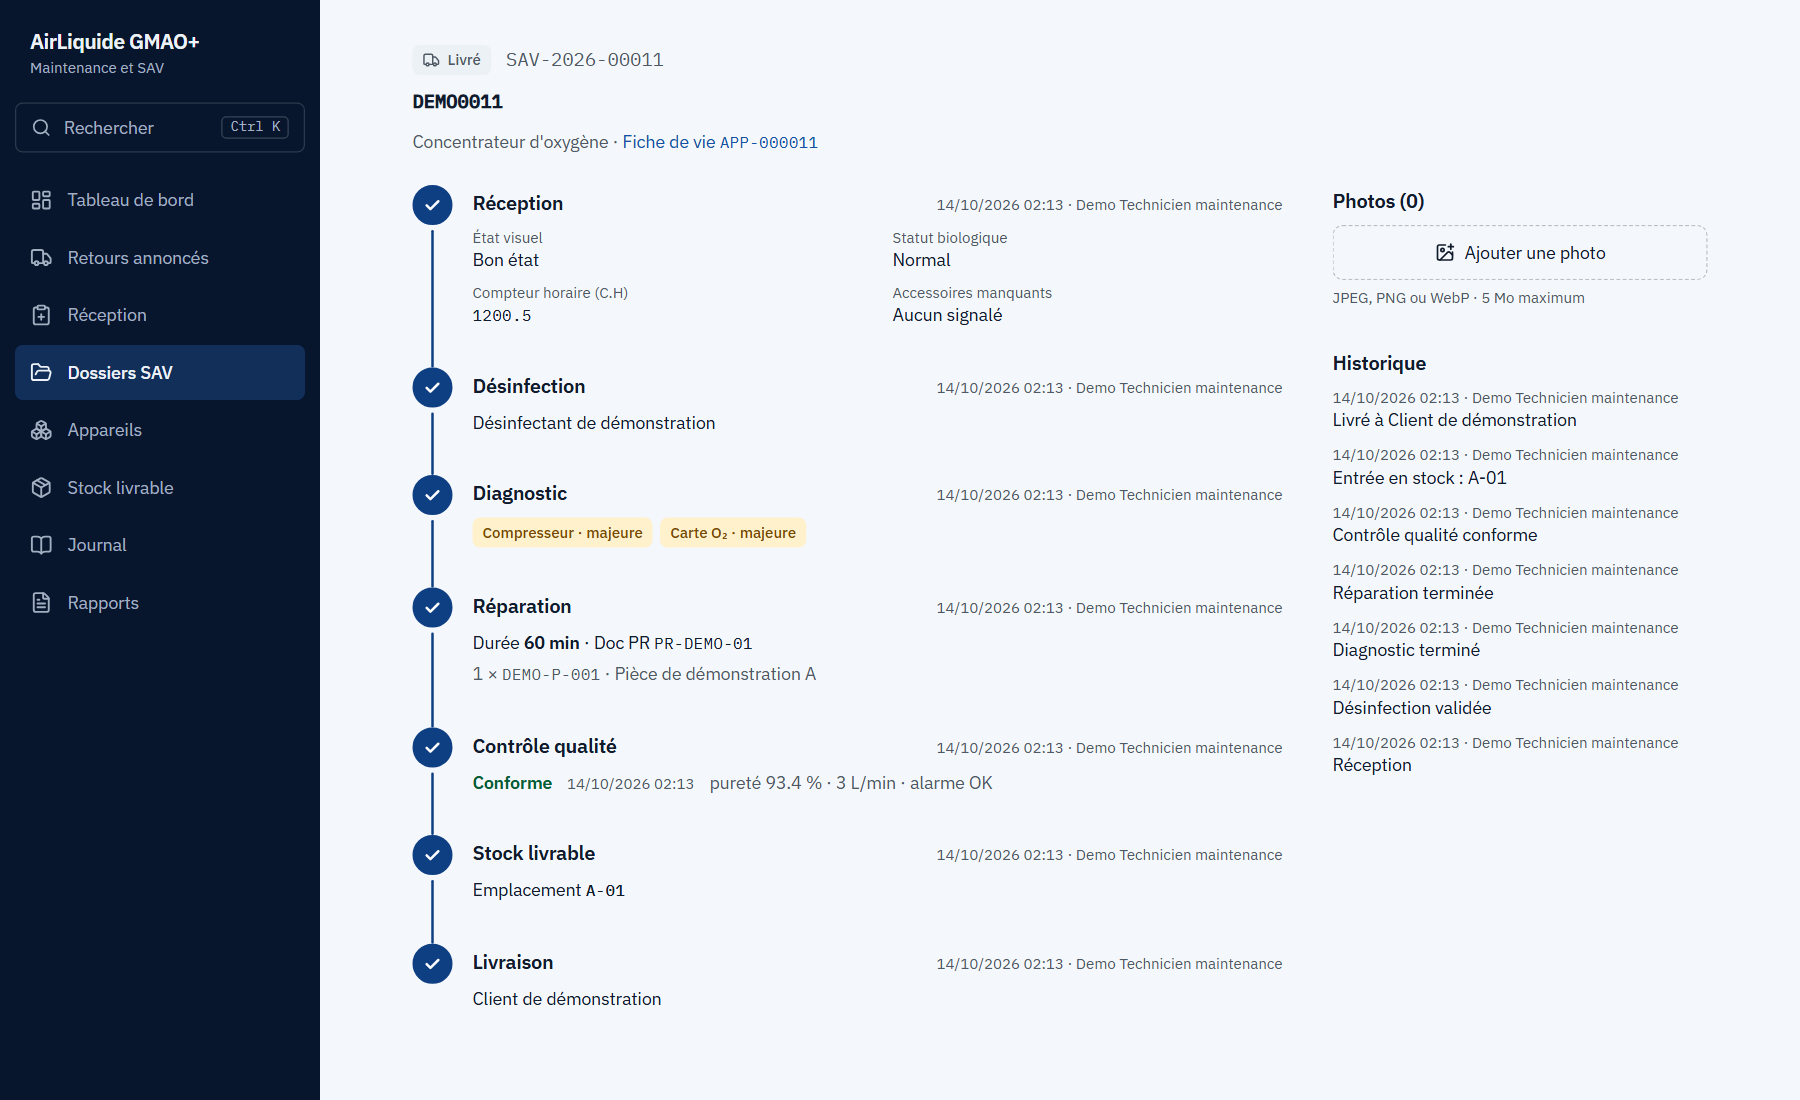
\includegraphics[width=15.0cm,height=17.5cm,keepaspectratio]{cap_dossier_livre.png}
\caption{Dossier livré : toutes les étapes sont résumées}
\end{figure}

Les captures de ce rapport ont été réalisées avec des \textbf{données de démonstration fictives}, clairement identifiées, et non avec des données réelles d'Air Liquide.


\chapter{Résultats obtenus et bilan}

\section{Tests réalisés}

La suite de tests automatisés du backend comprend \textbf{49 tests, tous réussis} lors de l'exécution du 28 octobre 2026 (environnement SQLite). Les mêmes tests avaient également réussi sur PostgreSQL 16 au cours du développement.

\Needspace{12\baselineskip}

{\small\setstretch{1.05}\renewcommand{\arraystretch}{1.3}\arrayrulecolor{ALtexte}
\begin{longtable}{|>{\raggedright\arraybackslash}p{4.00cm}|>{\raggedright\arraybackslash}p{2.23cm}|>{\raggedright\arraybackslash}p{8.01cm}|}
\caption{Répartition des tests automatisés du backend (total : 49)}\\
\hline
\rowcolor{ALbleu} \sffamily\bfseries\color{white} Thème & \sffamily\bfseries\color{white} Nombre de tests & \sffamily\bfseries\color{white} Ce qui est vérifié \\ \hline
\endfirsthead
\caption[]{Répartition des tests automatisés du backend (total : 49) (suite)}\\
\hline
\rowcolor{ALbleu} \sffamily\bfseries\color{white} Thème & \sffamily\bfseries\color{white} Nombre de tests & \sffamily\bfseries\color{white} Ce qui est vérifié \\ \hline
\endhead
Authentification et permissions & 12 & Connexion, refus d'accès, droits par rôle, cookie HttpOnly, renouvellement, déconnexion, limitation du débit \\ \hline
\rowcolor{ALgris} Réception et transitions & 10 & Création de l'appareil, doublons, saut d'étape interdit, retour arrière réservé, historique immuable \\ \hline
Étapes du workflow & 11 & Cycle complet, fiche de vie unique, ordre des étapes, contrôle non conforme, livraison sans stock \\ \hline
\rowcolor{ALgris} Photos & 3 & Image valide, fichier non image, type non autorisé \\ \hline
Questionnaire de retour & 7 & Création, identifiant unique, rattachement à la réception, double réception, incohérence de série, risque biologique \\ \hline
\rowcolor{ALgris} Journal et indicateurs & 6 & Colonnes du journal, filtres, export CSV, pureté hors limites, tableau de bord, accès aux rapports \\ \hline
\end{longtable}
}

Côté frontend, aucun test automatisé n'a été écrit : les contrôles disponibles sont la vérification des types TypeScript, l'analyse statique (lint) sans erreur et la compilation de production, complétés par des captures d'écran et des essais manuels. C'est une limite assumée de ce travail (§ 4.5).

\section{Résultats fonctionnels}

Le tableau suivant confronte les fonctionnalités à leur niveau de vérification.

\Needspace{15\baselineskip}

{\small\setstretch{1.05}\renewcommand{\arraystretch}{1.3}\arrayrulecolor{ALtexte}
\begin{longtable}{|>{\raggedright\arraybackslash}p{8.22cm}|>{\raggedright\arraybackslash}p{6.39cm}|}
\caption{Niveau de vérification des fonctionnalités}\\
\hline
\rowcolor{ALbleu} \sffamily\bfseries\color{white} Fonctionnalité & \sffamily\bfseries\color{white} Niveau de vérification \\ \hline
\endfirsthead
\caption[]{Niveau de vérification des fonctionnalités (suite)}\\
\hline
\rowcolor{ALbleu} \sffamily\bfseries\color{white} Fonctionnalité & \sffamily\bfseries\color{white} Niveau de vérification \\ \hline
\endhead
Authentification, rôles, limitation de débit & Implémentée, testée automatiquement \\ \hline
\rowcolor{ALgris} Fiche de vie unique, dossier unique ouvert & Implémentée, testée automatiquement \\ \hline
Workflow à 7 statuts et prérequis & Implémentée, testée automatiquement \\ \hline
\rowcolor{ALgris} Historique immuable & Implémentée, testée automatiquement \\ \hline
Désinfection, diagnostic, réparation, contrôle qualité, stock, livraison & Implémentée, testée automatiquement \\ \hline
\rowcolor{ALgris} Questionnaire de retour, journal de maintenance, exports CSV & Implémentée, testée automatiquement \\ \hline
Interface web (16 écrans, version mobile adaptée) & Implémentée, vérifiée par compilation, lint et captures \\ \hline
\rowcolor{ALgris} Rapports PDF, maintenance préventive, application mobile & Non réalisées \\ \hline
\end{longtable}
}

\section{Validation par les utilisateurs}

L'application a été testée par les techniciens du service, Fares et Maher, qui l'ont validée.

\Needspace{18\baselineskip}
\section{Difficultés rencontrées et solutions apportées}

{\small\setstretch{1.05}\renewcommand{\arraystretch}{1.3}\arrayrulecolor{ALtexte}
\begin{longtable}{|>{\raggedright\arraybackslash}p{6.85cm}|>{\raggedright\arraybackslash}p{7.76cm}|}
\caption{Principales difficultés techniques et solutions}\\
\hline
\rowcolor{ALbleu} \sffamily\bfseries\color{white} Difficulté & \sffamily\bfseries\color{white} Solution apportée \\ \hline
\endfirsthead
\caption[]{Principales difficultés techniques et solutions (suite)}\\
\hline
\rowcolor{ALbleu} \sffamily\bfseries\color{white} Difficulté & \sffamily\bfseries\color{white} Solution apportée \\ \hline
\endhead
Le modèle initial à entité unique \og{}Machine\fg{} ne distinguait pas l'appareil de ses retours & Séparation en appareil (fiche de vie) et dossier SAV, avec contrainte d'un seul dossier ouvert \\ \hline
\rowcolor{ALgris} Éviter les transitions incohérentes (par exemple livrer sans contrôle) & Services transactionnels : chaque étape vérifie le statut attendu et ses prérequis ; tests dédiés \\ \hline
Stockage des jetons dans le navigateur exposé aux scripts malveillants & Jeton de rafraîchissement en cookie HttpOnly, jeton d'accès en mémoire, limitation des tentatives \\ \hline
\rowcolor{ALgris} Erreur \og{}inconnue\fg{} affichée alors que la base n'était pas à jour (migration non appliquée) & Messages d'erreur explicites côté interface (serveur injoignable, erreur interne, migrations) \\ \hline
Polices téléchargées depuis un service externe, indisponibles sans réseau & Polices installées localement avec le projet (paquets \texttt{@fontsource}) \\ \hline
\rowcolor{ALgris} Contraintes d'une version récente de Next.js sur le rendu dynamique & Réorganisation de la mise en page (suspension du rendu) et contenu toujours rendu \\ \hline
Environnement Docker instable sur le poste de développement & Démarrage de Docker Desktop, base SQLite de repli, validation sur les deux bases \\ \hline
\end{longtable}
}

\section{Limites du travail}

\begin{itemize}
  \item pas de \textbf{rapports PDF} (exports CSV uniquement), alors que le cahier des charges les mentionnait ;
  \item pas de \textbf{maintenance préventive} ni de suivi des interventions correctives, pourtant présents dans le classeur existant (onglets PM\_\allowbreak{}LOG et CM\_\allowbreak{}LOG), ni de type de service ou de propriété de l'appareil ;
  \item \textbf{aucun test automatisé du frontend} ;
  \item l'exigence de \textbf{saisie en moins d'une minute} n'a pas été mesurée ;
  \item pas d'écran d'administration des utilisateurs et des catalogues (disponibles par l'API et l'administration Django) ;
  \item pas d'\textbf{application mobile}, pas de déploiement documenté en production ;
  \item les captures du rapport utilisent des données de démonstration et ne reflètent pas des volumes réels.
\end{itemize}

\section{Perspectives}

\begin{itemize}
  \item génération de \textbf{rapports PDF} et de statistiques avancées ;
  \item intégration de la \textbf{maintenance préventive} (dates de prochain service) et des types de service du classeur ;
  \item \textbf{import des données existantes} du classeur Google Sheets ;
  \item \textbf{application mobile} Flutter connectée à la même API ;
  \item conteneurisation complète, intégration continue et déploiement sécurisé ;
  \item tests automatisés de bout en bout du frontend ;
  \item étiquettes \textbf{QR code} pour retrouver un appareil par lecture.
\end{itemize}


\chapter*{Conclusion générale}
\addcontentsline{toc}{chapter}{Conclusion générale}
\markboth{Conclusion générale}{Conclusion générale}

Ce stage au sein du service Maintenance d'Air Liquide Tunisie a permis de concevoir et de réaliser AirLiquide GMAO+, une application qui remplace les saisies papier et tableur par un suivi unique de chaque appareil, de son retour à sa livraison. Les principaux apports sont une \textbf{fiche de vie unique} par appareil, une \textbf{traçabilité} horodatée et immuable, des \textbf{règles de workflow} appliquées par le serveur et vérifiées par 49 tests, ainsi qu'un journal de maintenance qui reprend le registre existant.

Sur le plan des compétences, le stage a mobilisé l'analyse de besoin avec des utilisateurs de terrain, la modélisation, le développement d'une API et d'une interface web, la sécurité applicative et la rédaction de tests. Il a aussi montré l'importance de comprendre le métier avant de coder : plusieurs choix, comme la séparation entre l'appareil et ses retours, viennent directement de l'observation du circuit réel.

Le travail présente des limites, détaillées au chapitre 4 : absence de rapports PDF, de maintenance préventive et de version mobile, et tests du frontend à compléter. Ces points constituent les perspectives naturelles du projet.

Sur le plan personnel, ce stage m'a permis de confronter ma formation de futur ingénieur en génie biomédical, parcours TTIS, à une situation de terrain : comprendre le circuit réel d'un dispositif médical dans un atelier de maintenance, puis le traduire en une application utilisable par les techniciens. J'y ai gagné en autonomie, en rigueur de documentation et en aisance pour dialoguer avec des utilisateurs dont le métier n'est pas l'informatique. Cette expérience confirme l'intérêt, pour un ingénieur biomédical, de maîtriser à la fois la maintenance des dispositifs médicaux et les outils numériques qui en assurent la traçabilité ; elle constitue une base solide pour mon projet professionnel dans la maintenance biomédicale et les systèmes d'information de santé.



% BIBLIOGRAPHIE ET WEBOGRAPHIE
{\small\setstretch{1.1}
\begin{thebibliography}{99}
\addcontentsline{toc}{chapter}{Bibliographie et webographie}

\bibitem{ref1}
Air Liquide, \og{}Air Liquide in brief\fg{} (histoire et chiffres du groupe). \url{https://www.airliquide.com/group/air-liquide-brief}. Consulté le 28 octobre 2026.

\bibitem{ref2}
Air Liquide, \og{}Air Liquide in Tunisia\fg{}. \url{https://www.airliquide.com/group/tunisia}. Consulté le 28 octobre 2026.

\bibitem{ref3}
Air Liquide Healthcare Tunisie, \og{}Qui sommes-nous\fg{}. \url{https://tn.healthcare.airliquide.com/propos-de-nous/qui-sommes-nous}. Consulté le 28 octobre 2026.

\bibitem{ref4}
Air Liquide Healthcare Tunisie, \og{}Équipements\fg{}. \url{https://tn.healthcare.airliquide.com/nos-solutions/equipements}. Consulté le 28 octobre 2026.

\bibitem{ref5}
Django Software Foundation, Documentation de Django. \url{https://docs.djangoproject.com/}

\bibitem{ref6}
Encode OSS, Django REST Framework. \url{https://www.django-rest-framework.org/}

\bibitem{ref7}
Vercel, Documentation de Next.js. \url{https://nextjs.org/docs}

\bibitem{ref8}
PostgreSQL Global Development Group, Documentation de PostgreSQL 16. \url{https://www.postgresql.org/docs/16/}

\bibitem{ref9}
Tailwind Labs, Documentation de Tailwind CSS. \url{https://tailwindcss.com/docs}

\bibitem{ref10}
shadcn, Documentation de shadcn/ui. \url{https://ui.shadcn.com/}

\bibitem{ref11}
Jones M., Bradley J., Sakimura N., \og{}JSON Web Token (JWT)\fg{}, RFC 7519, IETF, 2015. \url{https://datatracker.ietf.org/doc/html/rfc7519}
\end{thebibliography}
}

\vspace{0.6em}
\noindent\textit{Les sources ci-dessous sont celles réellement utilisées pour ce rapport. Les informations sur l'entreprise proviennent des pages officielles d'Air Liquide, consultées le 28 octobre 2026.}

\chapter*{Annexes}
\addcontentsline{toc}{chapter}{Annexes}
\markboth{Annexes}{Annexes}
\setcounter{table}{0}\setcounter{figure}{0}
\renewcommand{\thetable}{A.\arabic{table}}\renewcommand{\thefigure}{A.\arabic{figure}}
\setlength{\emergencystretch}{2em}

\Needspace{22\baselineskip}
\section*{Annexe A : Principaux points d'accès de l'API}
\addcontentsline{toc}{section}{Annexe A : Principaux points d'accès de l'API}

{\footnotesize\setstretch{1.05}\renewcommand{\arraystretch}{1.3}\arrayrulecolor{ALtexte}
\begin{longtable}{|>{\raggedright\arraybackslash}p{1.91cm}|>{\raggedright\arraybackslash}p{5.72cm}|>{\raggedright\arraybackslash}p{2.77cm}|>{\raggedright\arraybackslash}p{3.47cm}|}
\caption{Points d'accès de l'API}\\
\hline
\rowcolor{ALbleu} \sffamily\bfseries\color{white} Méthode & \sffamily\bfseries\color{white} Route & \sffamily\bfseries\color{white} Rôle & \sffamily\bfseries\color{white} Description \\ \hline
\endfirsthead
\caption[]{Points d'accès de l'API (suite)}\\
\hline
\rowcolor{ALbleu} \sffamily\bfseries\color{white} Méthode & \sffamily\bfseries\color{white} Route & \sffamily\bfseries\color{white} Rôle & \sffamily\bfseries\color{white} Description \\ \hline
\endhead
POST & \texttt{/\allowbreak{}api/\allowbreak{}auth/\allowbreak{}login/\allowbreak{}} & public & Connexion (jeton d'accès + cookie) \\ \hline
\rowcolor{ALgris} POST & \texttt{/\allowbreak{}api/\allowbreak{}auth/\allowbreak{}refresh/\allowbreak{}}, \texttt{/\allowbreak{}api/\allowbreak{}auth/\allowbreak{}logout/\allowbreak{}} & cookie & Renouvellement, déconnexion \\ \hline
GET & \texttt{/\allowbreak{}api/\allowbreak{}auth/\allowbreak{}me/\allowbreak{}} & connecté & Profil \\ \hline
\rowcolor{ALgris} CRUD & \texttt{/\allowbreak{}api/\allowbreak{}users/\allowbreak{}} & Responsable & Administration des utilisateurs \\ \hline
CRUD & \texttt{/\allowbreak{}api/\allowbreak{}device-\allowbreak{}types/\allowbreak{}}, \texttt{/\allowbreak{}brands/\allowbreak{}}, \texttt{/\allowbreak{}device-\allowbreak{}models/\allowbreak{}}, \texttt{/\allowbreak{}faults/\allowbreak{}}, \texttt{/\allowbreak{}parts/\allowbreak{}} & lecture : tous ; écriture : Responsable & Catalogues \\ \hline
\rowcolor{ALgris} GET & \texttt{/\allowbreak{}api/\allowbreak{}devices/\allowbreak{}?search=}, \texttt{/\allowbreak{}api/\allowbreak{}devices/\allowbreak{}\{id\}/\allowbreak{}life-\allowbreak{}sheet/\allowbreak{}} & connecté & Appareils et fiche de vie \\ \hline
POST / GET & \texttt{/\allowbreak{}api/\allowbreak{}returns/\allowbreak{}} & connecté & Questionnaire de retour \\ \hline
\rowcolor{ALgris} POST & \texttt{/\allowbreak{}api/\allowbreak{}dossiers/\allowbreak{}reception/\allowbreak{}} & connecté & Réception d'un appareil \\ \hline
POST & \texttt{/\allowbreak{}api/\allowbreak{}dossiers/\allowbreak{}\{id\}/\allowbreak{}disinfection/\allowbreak{}}, \texttt{/\allowbreak{}diagnosis/\allowbreak{}}, \texttt{/\allowbreak{}repair/\allowbreak{}}, \texttt{/\allowbreak{}quality-\allowbreak{}control/\allowbreak{}}, \texttt{/\allowbreak{}stock-\allowbreak{}entry/\allowbreak{}}, \texttt{/\allowbreak{}delivery/\allowbreak{}} & connecté & Étapes du workflow \\ \hline
\rowcolor{ALgris} POST & \texttt{/\allowbreak{}api/\allowbreak{}dossiers/\allowbreak{}\{id\}/\allowbreak{}transition/\allowbreak{}}, \texttt{/\allowbreak{}photos/\allowbreak{}} & connecté ; recul : Responsable & Transition contrôlée, photos \\ \hline
GET & \texttt{/\allowbreak{}api/\allowbreak{}dashboard/\allowbreak{}}, \texttt{/\allowbreak{}api/\allowbreak{}journal/\allowbreak{}}, \texttt{/\allowbreak{}api/\allowbreak{}stock-\allowbreak{}movements/\allowbreak{}} & connecté & Indicateurs, journal, mouvements \\ \hline
\rowcolor{ALgris} GET & \texttt{/\allowbreak{}api/\allowbreak{}reports/\allowbreak{}journal.\allowbreak{}csv}, \texttt{/\allowbreak{}api/\allowbreak{}reports/\allowbreak{}dossiers.\allowbreak{}csv} & connecté / Responsable & Exports CSV \\ \hline
\end{longtable}
}

\Needspace{16\baselineskip}
\section*{Annexe B : Entités du modèle de données}
\addcontentsline{toc}{section}{Annexe B : Entités du modèle de données}

{\small\setstretch{1.05}\renewcommand{\arraystretch}{1.3}\arrayrulecolor{ALtexte}
\begin{longtable}{|>{\raggedright\arraybackslash}p{3.65cm}|>{\raggedright\arraybackslash}p{10.96cm}|}
\caption{Entités du modèle de données}\\
\hline
\rowcolor{ALbleu} \sffamily\bfseries\color{white} Groupe & \sffamily\bfseries\color{white} Entités \\ \hline
\endfirsthead
\caption[]{Entités du modèle de données (suite)}\\
\hline
\rowcolor{ALbleu} \sffamily\bfseries\color{white} Groupe & \sffamily\bfseries\color{white} Entités \\ \hline
\endhead
Utilisateurs & User (rôles : technicien, responsable SAV) \\ \hline
\rowcolor{ALgris} Référentiel d'appareils & DeviceType, Brand, DeviceModel, Device \\ \hline
Retour et dossier & ReturnDeclaration, DossierSAV, StatusHistory \\ \hline
\rowcolor{ALgris} Étapes du dossier & Disinfection, Diagnosis, DetectedFault, Repair, ReplacedPart, QualityControl, StockMovement, Delivery, Photo \\ \hline
Catalogues & Fault (pannes par type d'appareil), Part (pièces) \\ \hline
\rowcolor{ALgris} Énumérations & VisualCondition, BiohazardStatus \\ \hline
\end{longtable}
}

\Needspace{15\baselineskip}
\section*{Annexe C : Organisation du dépôt}
\addcontentsline{toc}{section}{Annexe C : Organisation du dépôt}

{\small\setstretch{1.05}\renewcommand{\arraystretch}{1.3}\arrayrulecolor{ALtexte}
\begin{longtable}{|>{\raggedright\arraybackslash}p{3.65cm}|>{\raggedright\arraybackslash}p{10.96cm}|}
\caption{Organisation du dépôt}\\
\hline
\rowcolor{ALbleu} \sffamily\bfseries\color{white} Dossier & \sffamily\bfseries\color{white} Contenu \\ \hline
\endfirsthead
\caption[]{Organisation du dépôt (suite)}\\
\hline
\rowcolor{ALbleu} \sffamily\bfseries\color{white} Dossier & \sffamily\bfseries\color{white} Contenu \\ \hline
\endhead
\texttt{backend/\allowbreak{}} & Applications Django : accounts, inventory, maintenance, dashboard, reports, common ; configuration \\ \hline
\rowcolor{ALgris} \texttt{frontend/\allowbreak{}} & Application Next.js : pages, composants, bibliothèque d'appels à l'API \\ \hline
\texttt{docs/\allowbreak{}} & Vision, cahier des charges, workflow, cas d'utilisation, architecture, base de données, API, démarrage, captures \\ \hline
\rowcolor{ALgris} \texttt{docs/\allowbreak{}diagrams/\allowbreak{}} & Sources des diagrammes UML (PlantUML, Mermaid) \\ \hline
\texttt{docker-\allowbreak{}compose.\allowbreak{}yml} & Base de données PostgreSQL 16 \\ \hline
\end{longtable}
}

\Needspace{22\baselineskip}
\section*{Annexe D : Correspondance entre le journal papier et l'application}
\addcontentsline{toc}{section}{Annexe D : Correspondance entre le journal papier et l'application}

{\small\setstretch{1.05}\renewcommand{\arraystretch}{1.3}\arrayrulecolor{ALtexte}
\begin{longtable}{|>{\raggedright\arraybackslash}p{5.02cm}|>{\raggedright\arraybackslash}p{9.59cm}|}
\caption{Correspondance journal papier / application}\\
\hline
\rowcolor{ALbleu} \sffamily\bfseries\color{white} Colonne du journal papier & \sffamily\bfseries\color{white} Origine dans AirLiquide GMAO+ \\ \hline
\endfirsthead
\caption[]{Correspondance journal papier / application (suite)}\\
\hline
\rowcolor{ALbleu} \sffamily\bfseries\color{white} Colonne du journal papier & \sffamily\bfseries\color{white} Origine dans AirLiquide GMAO+ \\ \hline
\endhead
Année, Mois & Date de réception du dossier \\ \hline
\rowcolor{ALgris} Équip. / type & Type d'appareil et modèle \\ \hline
N° série & Appareil (numéro normalisé) \\ \hline
\rowcolor{ALgris} C.H & Compteur horaire saisi à la réception \\ \hline
Pureté & Contrôle qualité (pureté O\textsubscript{2}, de 0 à 100 \%) \\ \hline
\rowcolor{ALgris} Débit / pression & Contrôle qualité \\ \hline
Alarme sonore & Contrôle qualité (conforme, non conforme, non testée) \\ \hline
\rowcolor{ALgris} Pannes & Diagnostic (pannes du catalogue) \\ \hline
Doc de sortie PR & Réparation (référence du document de sortie des pièces) \\ \hline
\rowcolor{ALgris} Technicien & Technicien de la réparation, à défaut de la désinfection \\ \hline
Date sortie & Date de livraison \\ \hline
\end{longtable}
}

Hypothèses à valider avec le service : \og{}C.H\fg{} désigne le compteur horaire ; \og{}Doc de sortie PR\fg{} désigne le document de sortie de pièces de rechange ; le dernier contrôle qualité fait foi pour les mesures.

\section*{Annexe E : Captures complémentaires}
\addcontentsline{toc}{section}{Annexe E : Captures complémentaires}

\begin{figure}[!htb]
\centering
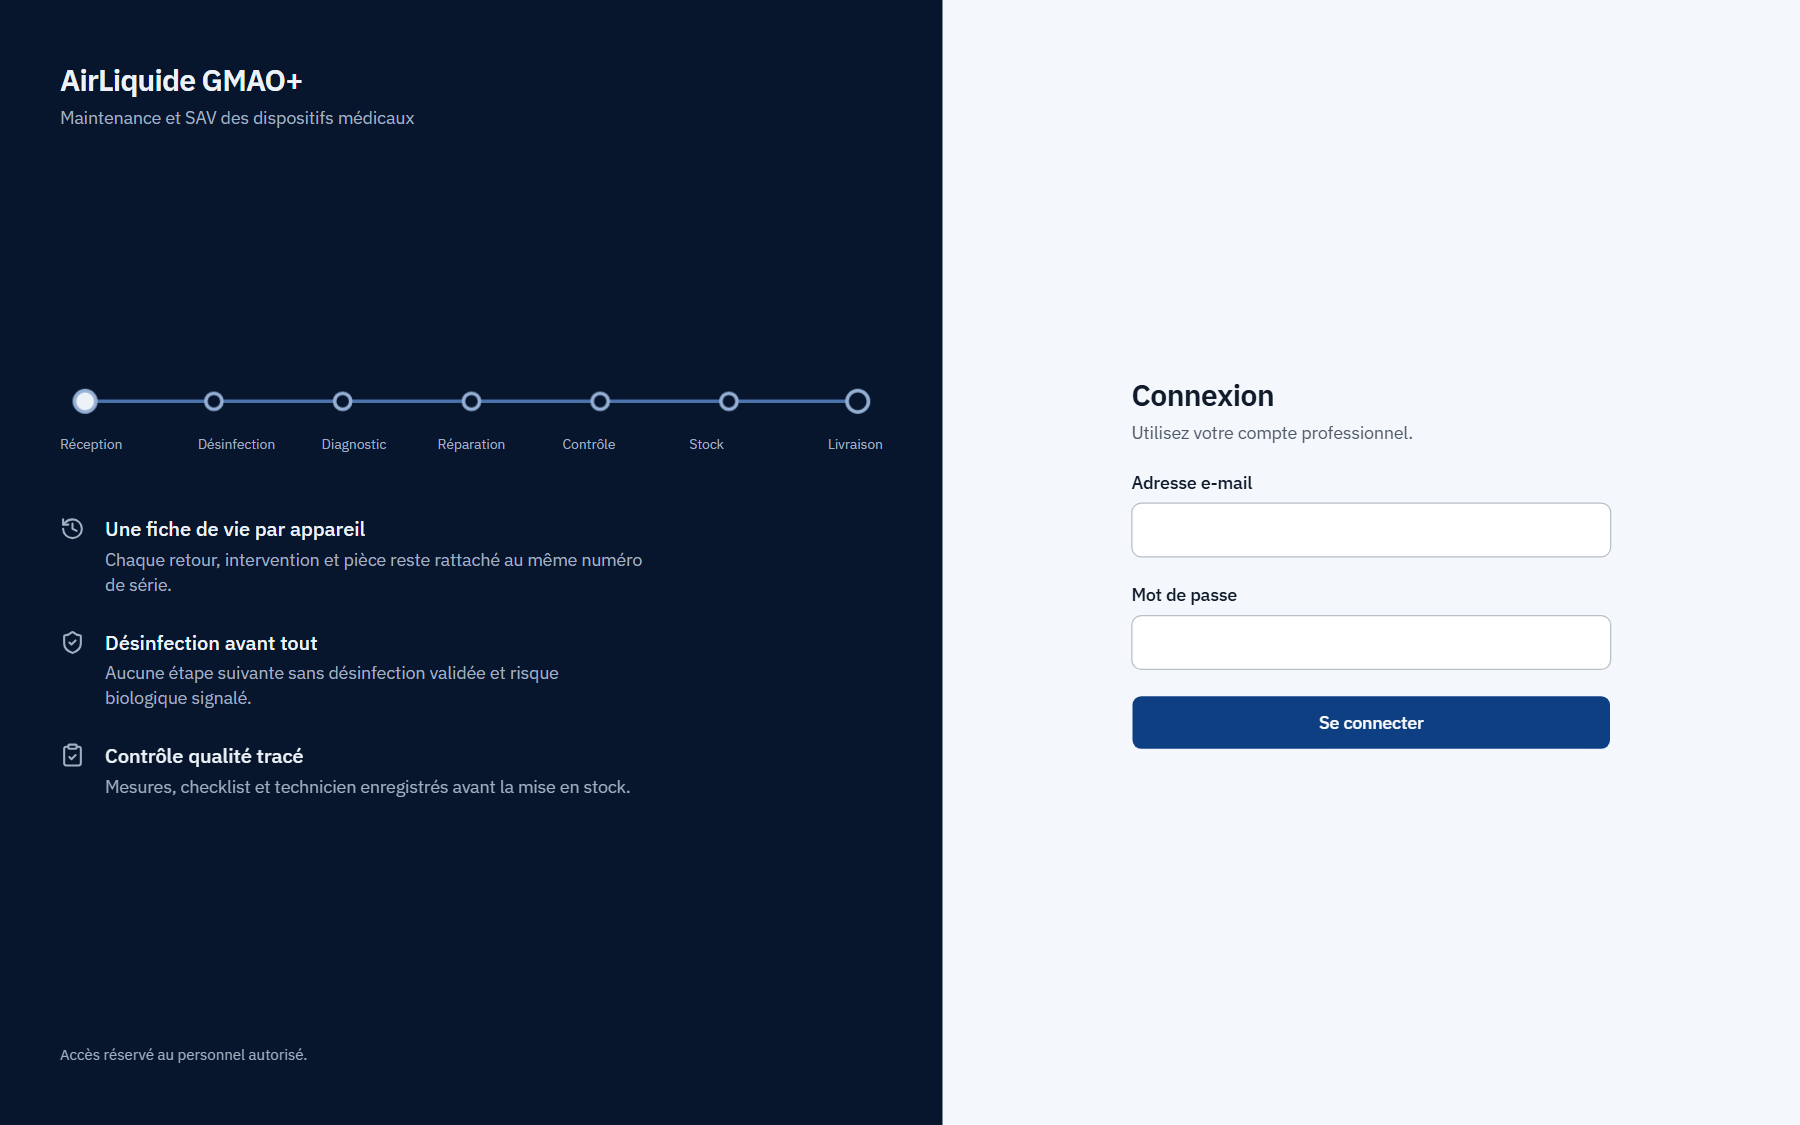
\includegraphics[width=15.0cm,height=17.5cm,keepaspectratio]{cap_connexion.png}
\caption{Écran de connexion}
\end{figure}

\begin{figure}[!htb]
\centering
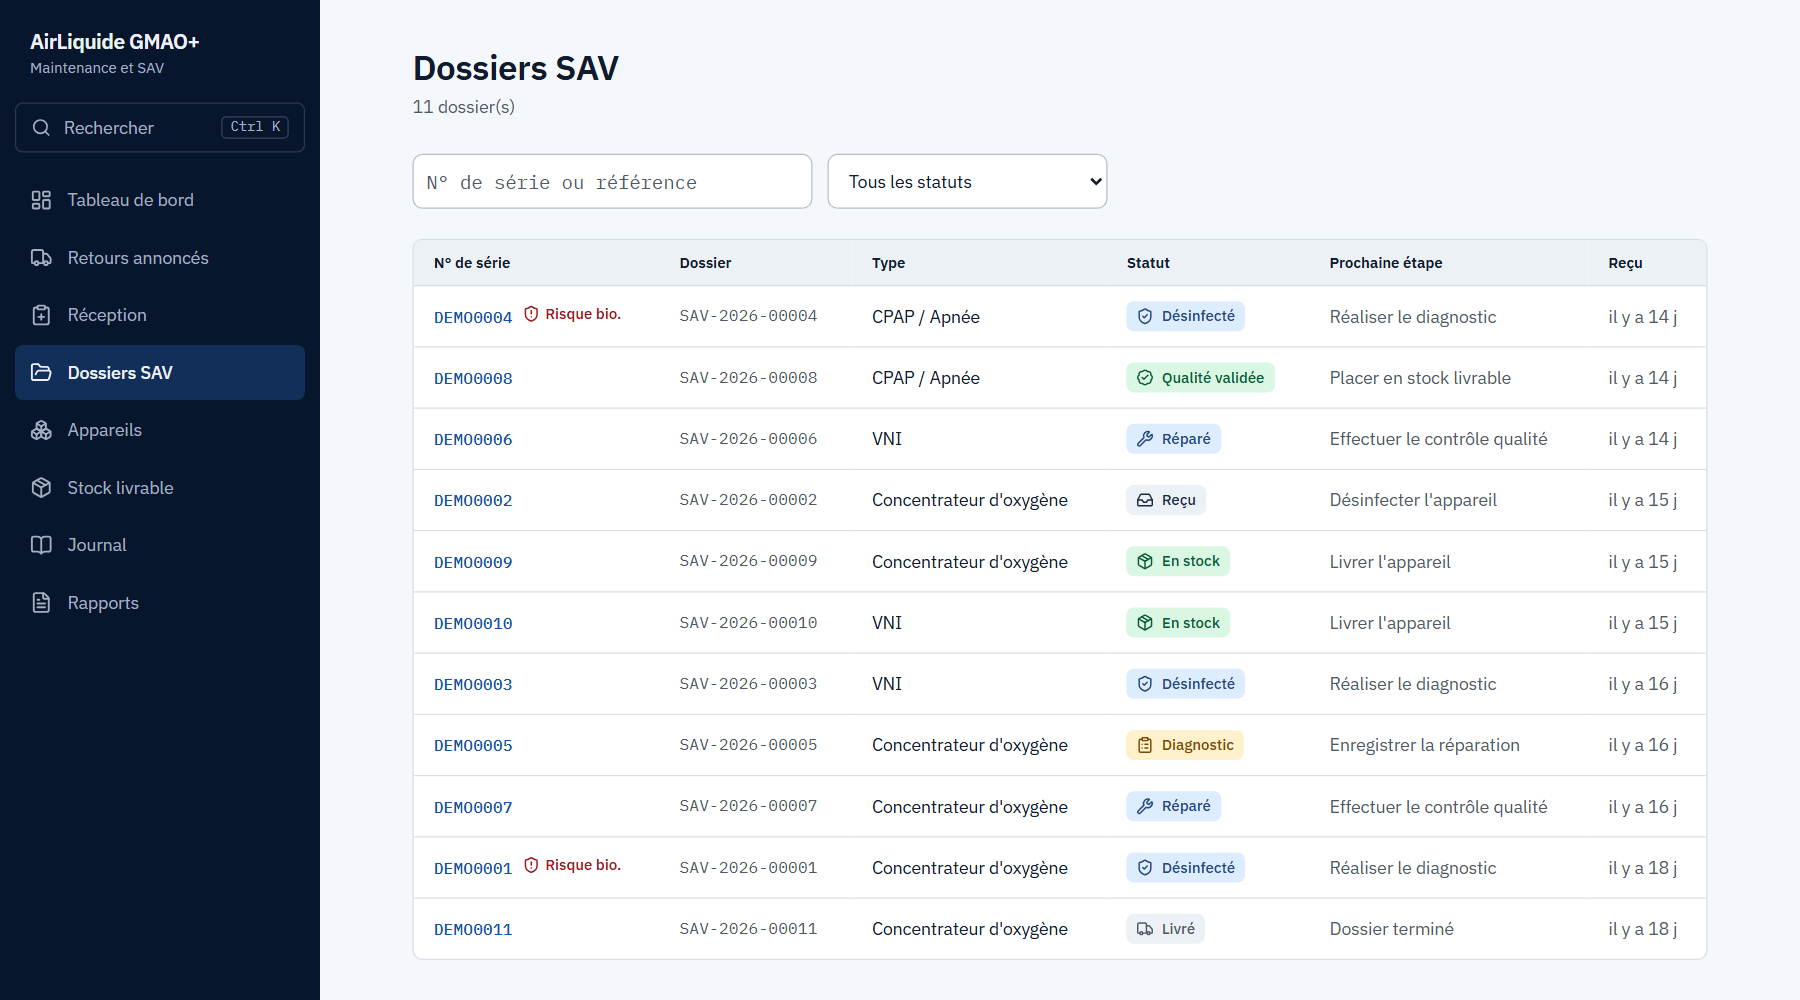
\includegraphics[width=15.0cm,height=17.5cm,keepaspectratio]{cap_dossiers.png}
\caption{Liste des dossiers SAV (données de démonstration)}
\end{figure}

\begin{figure}[!htb]
\centering
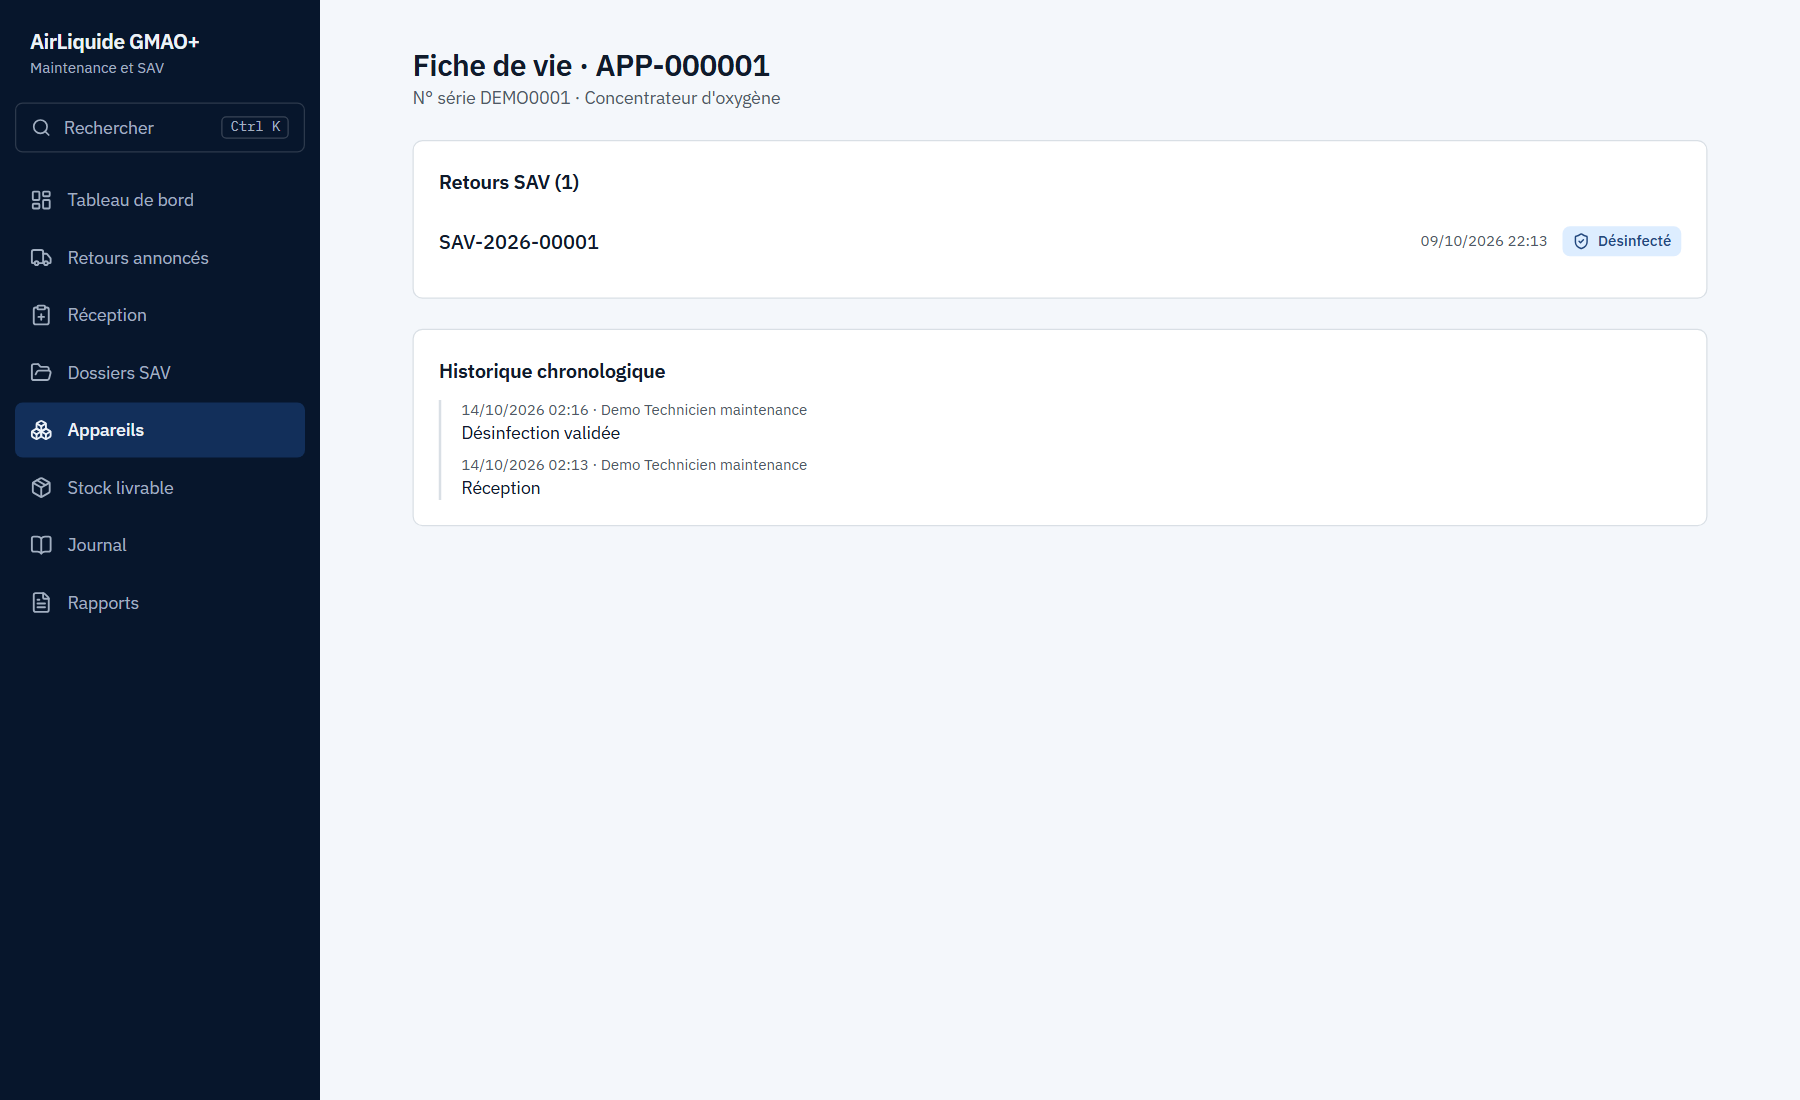
\includegraphics[width=15.0cm,height=17.5cm,keepaspectratio]{cap_fiche_vie.png}
\caption{Fiche de vie d'un appareil (données de démonstration)}
\end{figure}

\begin{figure}[!htb]
\centering
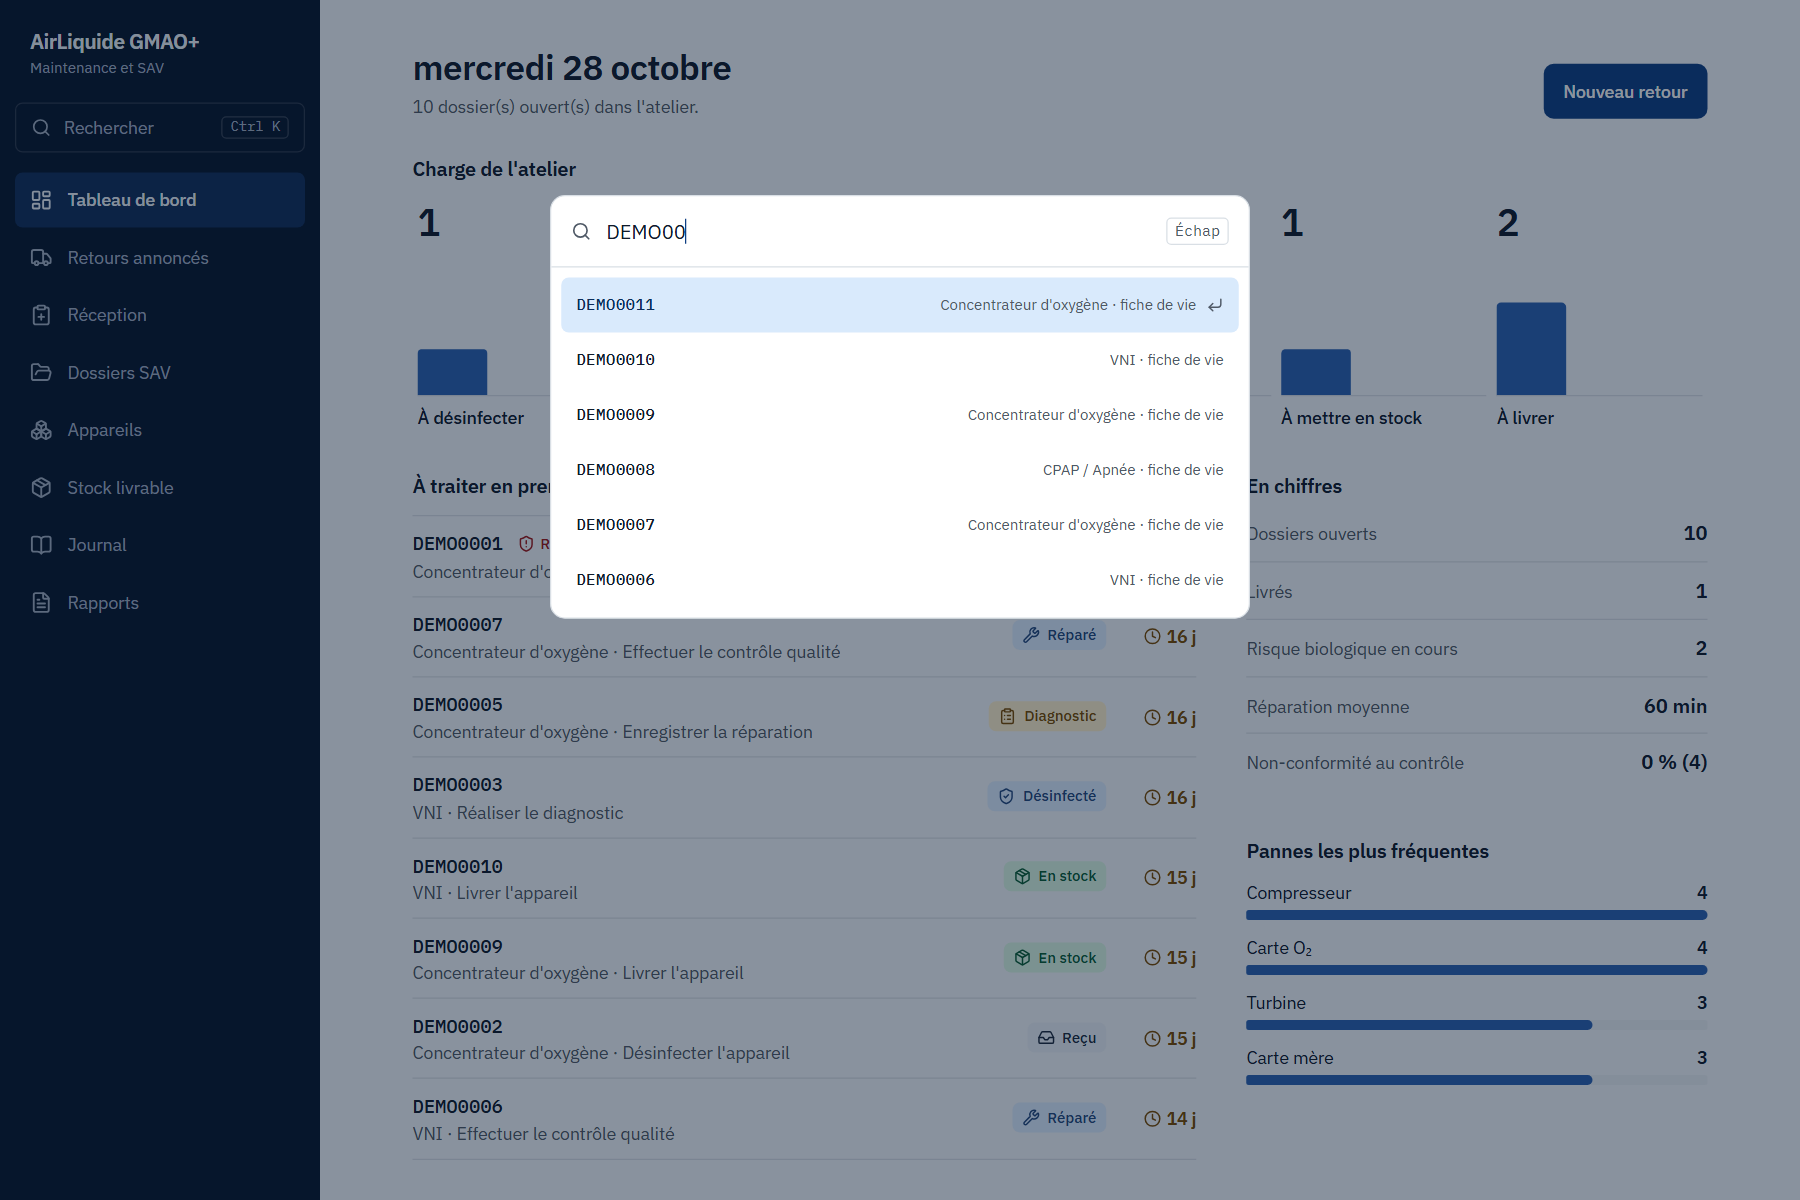
\includegraphics[width=15.0cm,height=17.5cm,keepaspectratio]{cap_palette.png}
\caption{Recherche rapide par numéro de série (Ctrl + K)}
\end{figure}

\begin{figure}[!htb]
\centering
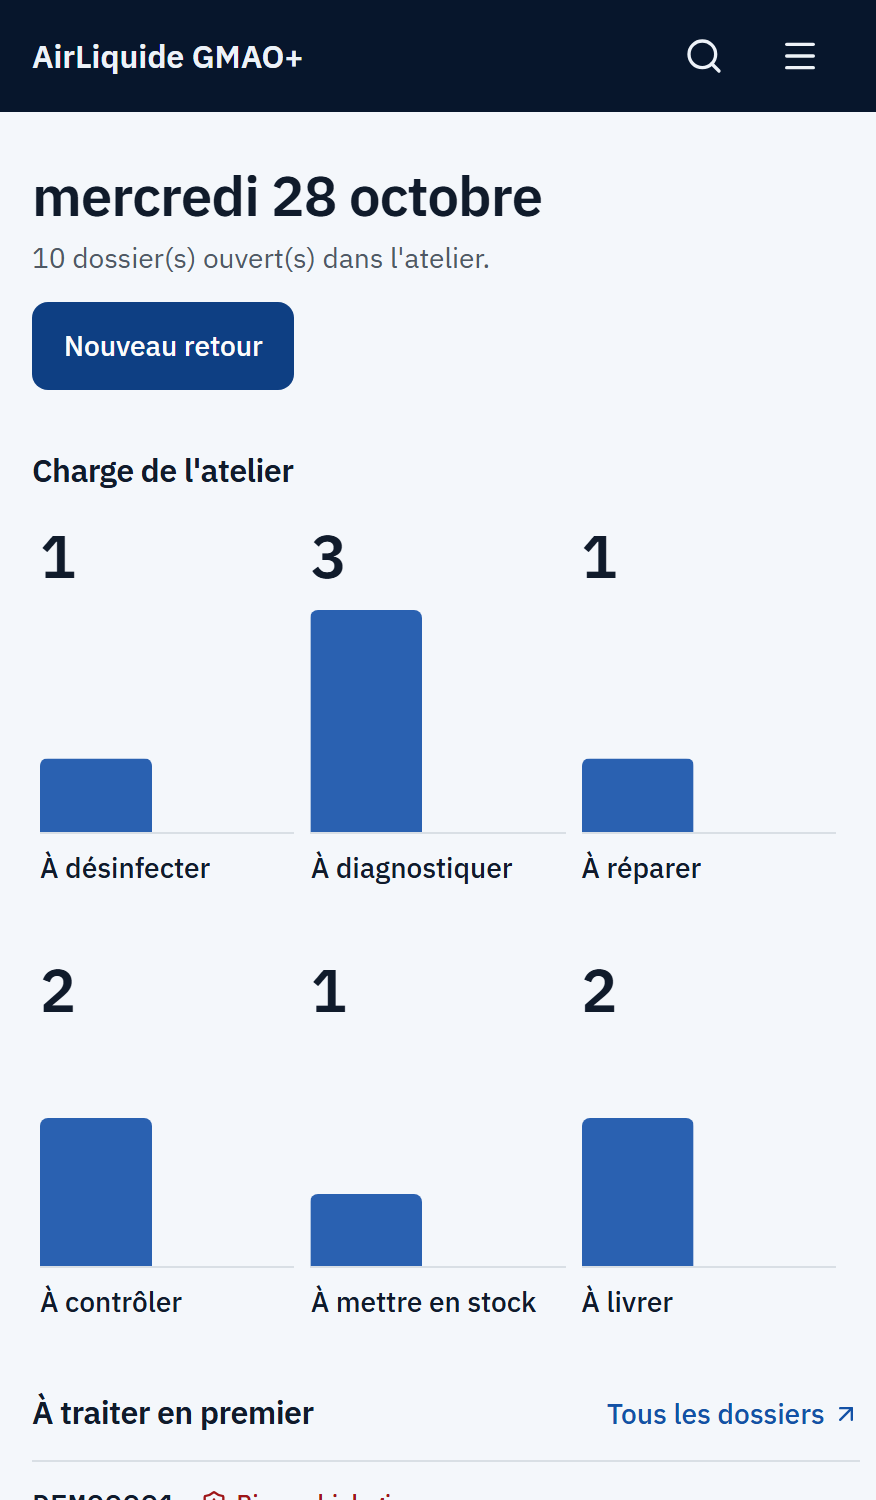
\includegraphics[width=7.5cm,height=17.0cm,keepaspectratio]{cap_mobile.png}
\caption{Tableau de bord sur téléphone}
\end{figure}

\section*{Annexe F : Exécution des tests automatisés}
\addcontentsline{toc}{section}{Annexe F : Exécution des tests automatisés}

Commande (depuis le dossier \texttt{backend/\allowbreak{}}) :

\texttt{python manage.\allowbreak{}py test}

Résultat observé le 28 octobre 2026, environnement SQLite : \texttt{Ran 49 tests} suivi de \texttt{OK}.



\end{document}
